% \documentclass[12pt,endfloats]{article}%
\documentclass[nofootinbib,preprint,floatfix,titlepage,endfloats,superscriptaddress]{revtex4} %  ,endfloats,floatfix
%\documentclass[12pt,a4paper,final]{iopart}
% \documentclass[nofootinbib,floatfix,reprint,prl,endfloats,superscriptaddress]{revtex4} %  ,floatfix

\usepackage[utf8]{inputenc}
\usepackage{nima,graphicx,amsmath,amssymb,color}%,hyperref}
\usepackage{mathrsfs}
%\usepackage{graphicx}
\usepackage{comment}
% \newcommand{\Ls}{\mathscr{L}}

\usepackage{setspace}
\linespread{1.5}

\newcommand{\lrto}{\leftrightarrow}
\marginparwidth 0pt
\oddsidemargin  0pt
\evensidemargin  0pt
\marginparsep 0pt
\topmargin   -0.25in 
\textwidth   6.5in
\textheight  9.0in
\newcommand{\RNum}[1]{\uppercase\expandafter{\romannumeral #1\relax}}
\newcommand{\outNim}[1]{}
%
% \documentclass{article}
\usepackage{array}

\begin{document}
%\begin{table}%[]
    \centerline{
    \begin{tabular}{|>{\bfseries}l|c|c|c|}
    \hline
        {\bf Nature} &\textbf{ Letters }& \textbf{Article} & \textbf{Ours}  \\
        \hline 
Abstract (words) & 200-300 &  500 & 286 \\
\hline 
Summary & 1 sentence ``we show'' & 150 words & - \\ 
\hline 
Text (words) & 1500 & 3000 & 2800\\
\hline 
Figures & 3-4 small & 5-6 normal & 4 large \\
\hline 
Pages & 4 & 5 & $\sim 3.5$ text, no figs \\
\hline 
References & $< 30$ & - & 45 \\
\hline 
    \end{tabular}
}
    %\caption
    \medskip{}
    
    {\bf \scriptsize Our current text is $\sim$2800 words and satisfies the Article format, but would need significant cuts to fit Letter. With the font and page size of PRL, the text alone becomes 3.5 pages. Adding figures would make it roughly 5. }
    %\label{tab:nature}

\vspace{4cm}
%\end{table}

%\end{document}
%\title{Phases of Physical 3D Networks}
\author{Nima Dehmamy\thanks{nidami@gmail.com}}
\affiliation{Center for Complex Network Research, Northeastern University, Boston, USA}
\author{Soodabeh Milanlouei}
\affiliation{Center for Complex Network Research, Northeastern University, Boston, USA}
\author{Albert-L\'aszl\'o Barab\'asi}
\affiliation{Center for Complex Network Research, Northeastern University, Boston, USA}
\affiliation{Center for Cancer Systems Biology, Dana Farber Cancer Institute, Boston, USA}
\affiliation{Department of Medicine, Brigham and Women’s Hospital, Harvard Medical School, Boston, USA}
\affiliation{Center for Network Science, Central European University, Budapest, Hungary}
%\maketitle
\date{\today}
% \maketitle
\centerline{\Huge Phases of Physical 3D Networks}
\outNim{
\medskip
\centerline{Nima Dehmamy\footnote{nidami@gmail.com}, Soodabeh Milanlouei, Albert-L\'aszl\'o Barab\'asi}
\centerline{\today}
\bigskip
}
  \begin{abstract}
% \begin{document}
{\bf 
Many physical networks, from neurons in a brain to bundles of cables carrying power in infrastructural systems, the nodes and links are physical objects unable to cross each other.
The layout and physical embeddedness of these networks is determined by these non-crossing conditions, limiting how they form and evolve. 
Current network layout algorithms, by ignoring the physical reality of the links and nodes, are inherently unable to model the characteristics of such physical networks. 
% By ignoring the physical reality of the links and nodes,
Here, we develop a model that accurately captures the physical reality of nodes and links, allowing us to 
%develop and study a series of 3D layout models that observe the physical constraints we encounter when nodes and links have true dimensions, allowing us to 
understand how they affect the layout of physical networks. 
We show that for small link thicknesses conflicts are rare, hence networks are in a weakly interacting phase, where links bend locally to avoid crossings without altering the overall network layout. 
Once, however, link thickness reaches a critical threshold, networks transition to a strongly interacting phase, in which  excluded volume interactions shape the network layout. 
We derive the scaling of this transition point, and show that a set of geometric quantities, from total link length to link curvature, alter their scaling behavior at the predicted transition point. 
At the same time we document a deep universality in each phase, finding that the network layout, geometric characteristics, and scaling are largely independent of the underlying network topology. 
Finally, we show that the transition point also affects the physical properties of the network: networks respond to external stress in a gel-like fashion in the strongly interacting phase, whereas in the weakly interacting phase they develop solid-like properties. 
These findings not only unveil the fundamental constraints real networks obey, but have direct implications in the layout of mammalian brains and for the 3D printing of realistic networks.
} % bf
\end{abstract}
\maketitle
%\end{document}

\newpage
\outNim{
Analyzing networks embedded in 3D space is crucial for understanding brain anatomy and pathologies pertaining to physical connections in the brain. 
Devising physical 3D layouts for networks is also of interest for  visualization purposes.
Additionally, given the recent advancements in 3D printing technology, 3D layouts may have practical value in design and manufacturing of complex devices. 
It is important to have efficient and economical 3D layout algorithm for networks. 
The role of network topology in layouts and the limitations it imposes on the feasibility of layouts must, thus, be studied.
We develop a minimal 3D layout algorithm for networks, inspired by force-directed layouts. 
We analyze the spatial properties of our layouts and find two phases based on link thickness and derive the phase transition criterion.  
In both phases, different network topologies turn out to be very similar in their volumetric properties and are not distinguishable based on volume. 
Relative link orientation, does differentiate the topologies when links are thin, but fails to do so at large link thickness. 
Thus, we discover a universal phase for 3D networks when link thickness is large.
We also evaluate the response of the layouts too stress. 
We find that even in terms of response to stress the different topologies behave the same in the universal phase. 
Additionally we find that the layouts behave like fluids in this phase. 
Comparing against brain literature, we find that many mammalian brains may be related to this universal phase at the level of connections between large brain regions.  
We also argue that primate brains most likely do not belong to this universal phase. 
}

Virtually, all network layout models in use are variants of the Force-Directed Layout (FDL) algorithm \cite{kamada1989algorithm,davidson1996drawing,fruchterman1991graph,barnes1986hierarchical}, which assigns spring-like attractive forces between linked node pairs to minimize the distance between them, and adds repulsive forces between all node pairs to ensure that the network does not collapse  
 \cite{kabourov2015spring}.
As FDL assumes dimensionless nodes and links, node overlap or link crossing have no impact on the layout. 
Consequently, FDL-based models are inherently incapable of capturing the properties of densely packed physical networks, like neurons in the brain \cite{kasthuri2015saturated,oh2014mesoscale}, underground hyphal networks \cite{friese1991spread,bago1998architecture}, or a bundle of wires in computer systems.
If we do consider the physical dimensions of the nodes and links, FDL leads to multiple link crossings or conflicts (Fig. \ref{fig:crs-lat}A), whose number increases linearly with link thickness $r_L$, and saturates for large $r_L$ (Fig. \ref{fig:crs-lat}B), a behavior predicted by a simple geometric model (SI, sec. \ref{ap:cross}). 
In physical networks, where such crossings are prohibited, a proper layout must systematically avoid these conflicts.
\begin{figure}
    %\vspace{4cm}
    \centering
    % 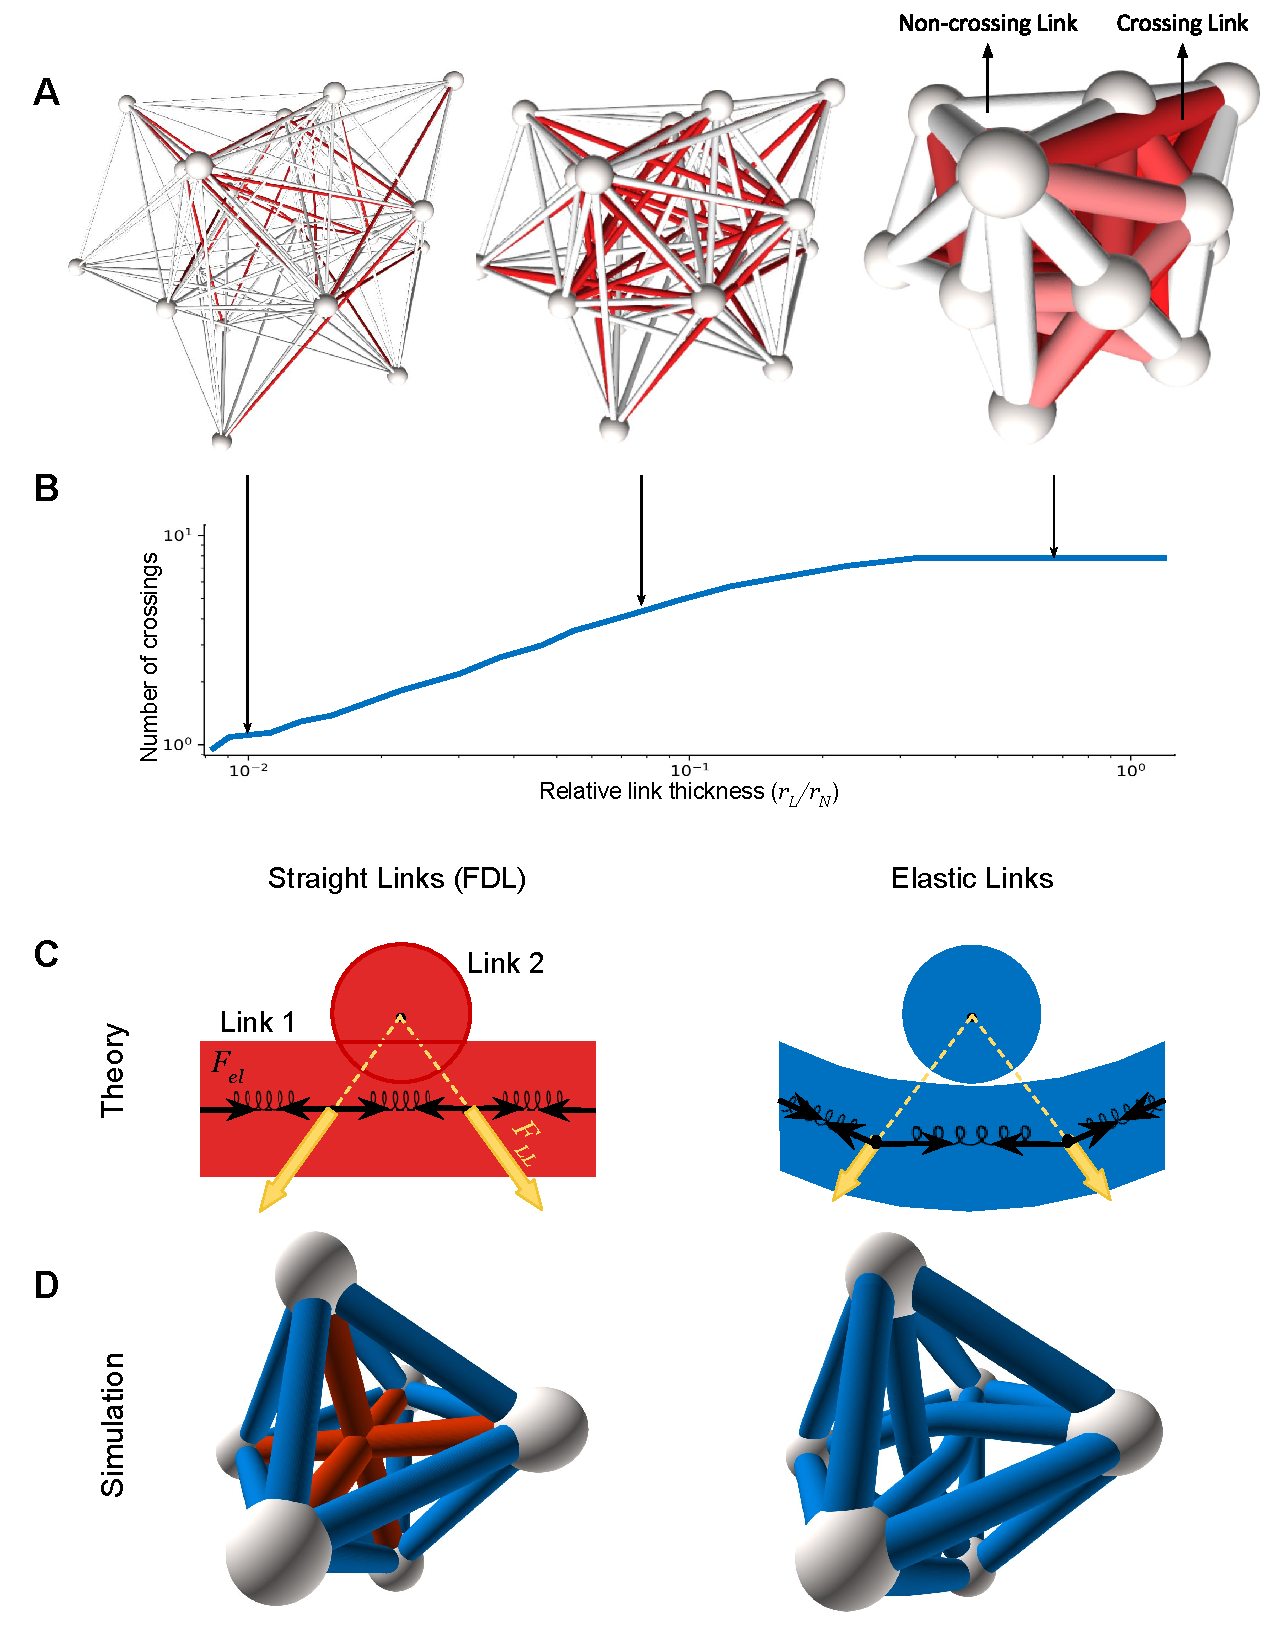
\includegraphics[width=.9\columnwidth]{fig-09-19/crs-resolve-0517.pdf}
    % 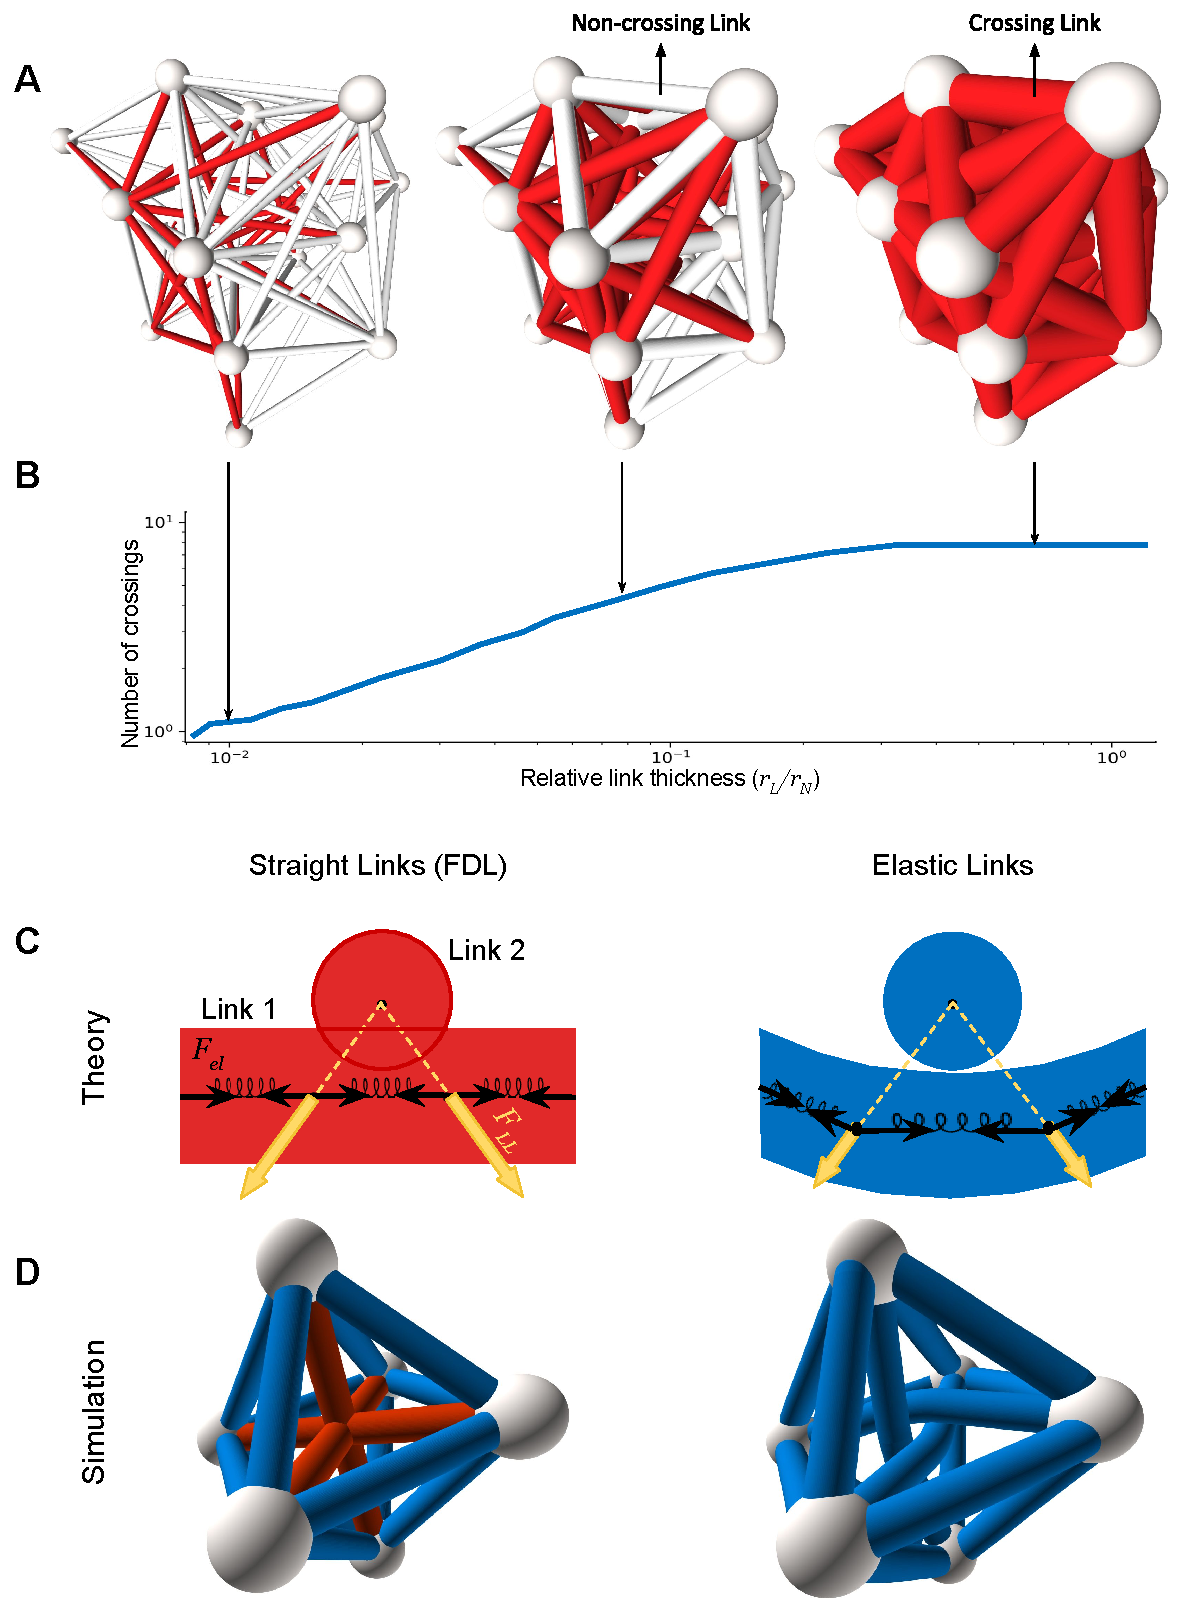
\includegraphics[width=.8\columnwidth]{fig-09-19/crs-resolve-061717.pdf}
    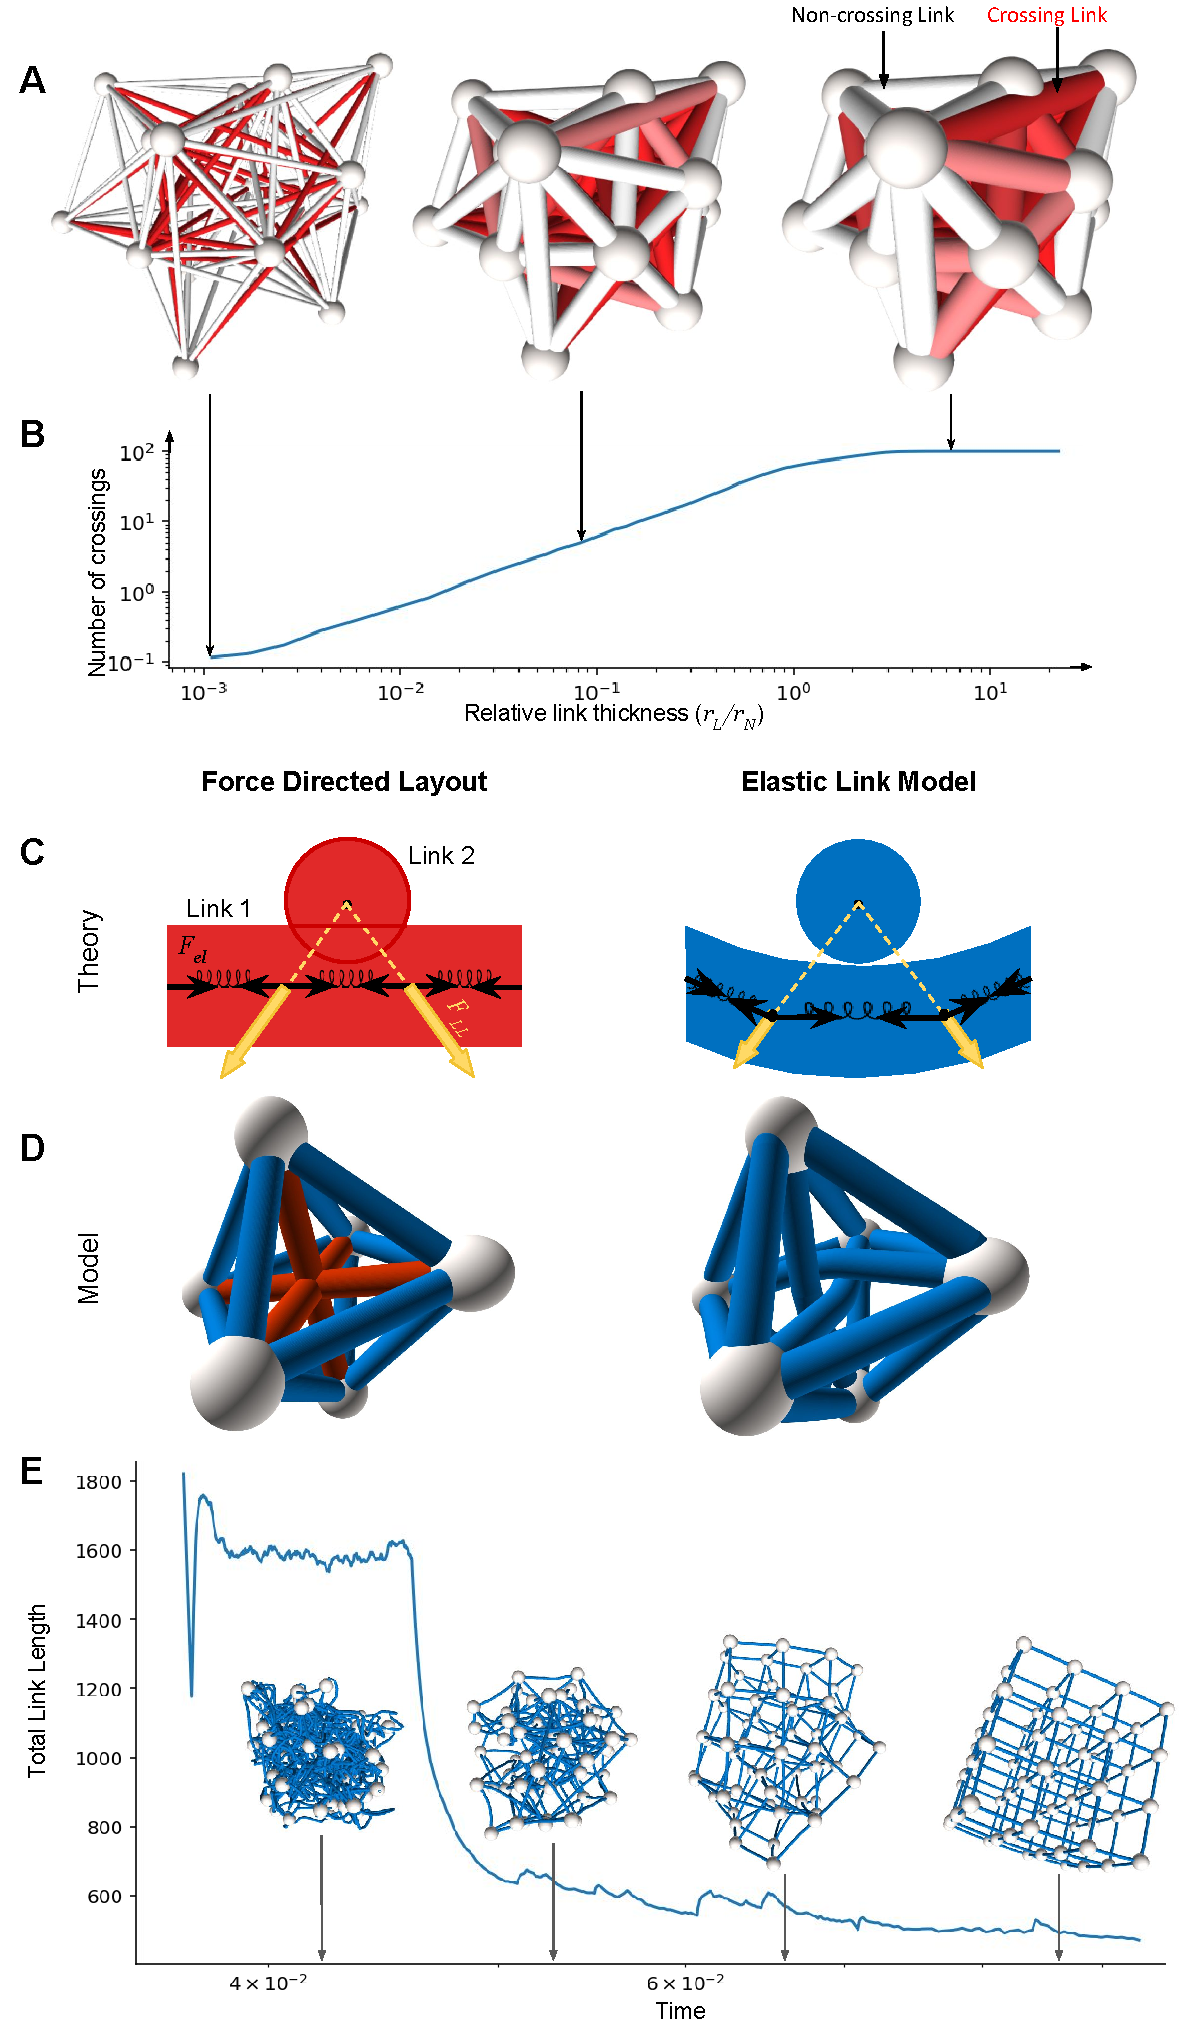
\includegraphics[width=.7\columnwidth]{fig-09-19/crs-lattice-071917.pdf}
    \caption{\scriptsize
    {\bf (A)}  Crossing links for a Barabasi-Albert (BA) network ($N = 20, m = 3$) in space, drawn by FDL. While increasing the link thickness $r_L$, the network occupies more space and crossings increase. 
    {\bf (B)} The plot shows the trend by which the number of crossings increases in a BA network with $N=100, m =3$ laid out in 3D using FDL.
    The number of crossings increases linearly with $r_L$ at first, before tapering off due to finiteness of the network. It can be shown (SI sec.\ref{ap:cross}) that layouts which result in random link orientations yield such linear trend in the growth of the number of crossings.
    {\bf(C) How ELI works:} We simulate the elastic links as a stretched, flexible rubber band, which can be thought of as many short springs connected to each other. 
    The elastic force $F_{el}$ of each spring is shown by black arrows.
    Links exert a repulsive force $F_{LL}$  on each other that falls sharply at radii larger than $r_L$. 
    First and second plot show how the ELI resolves crossing (red) links. {\bf(D)} shows a complete network with 6 nodes. Image on the left is laid out with FDL. The three red links all cross at the center. The right plot shows how the network looks after simulating ELI on it, after which the crossing is resolved.
    {\bf E} Simulation of the layout of a lattice with $r_L\ll r_N$. The link thickness corresponds to the actual thicknesses, while the node size is chosen based on proper visibility. Choosing short-range repulsion for nodes is crucial for getting a perfect lattice layout. Long range forces, e.g. electrostatic,  distort the layout at the boundaries. The plot shows the evolution of the total link length over time during the simulation, with several snapshots of the actual layout shown above each stage of the evolution. 
    The simulation started from a completely random layout. 
    We use simulated annealing to find the layout.
    Initially the thermal noise results in a very large total edge length, but it helps links pass through each other and thus resolve crossings.
    Still, in later stages the system is prone to get stuck in one of many local minima of the potential energy and not completely unfold. 
    To let the system unfold completely, we have exploited the discreteness and chose the number of link segments to be small. 
    This decreases the energy penalty of jumping from one local minimum to another and makes it more likely for the system to relax completely.
    }     
    \label{fig:crs-lat}
\end{figure}

\outNim{
\begin{figure}
    %\vspace{4cm}
    \centering
    % 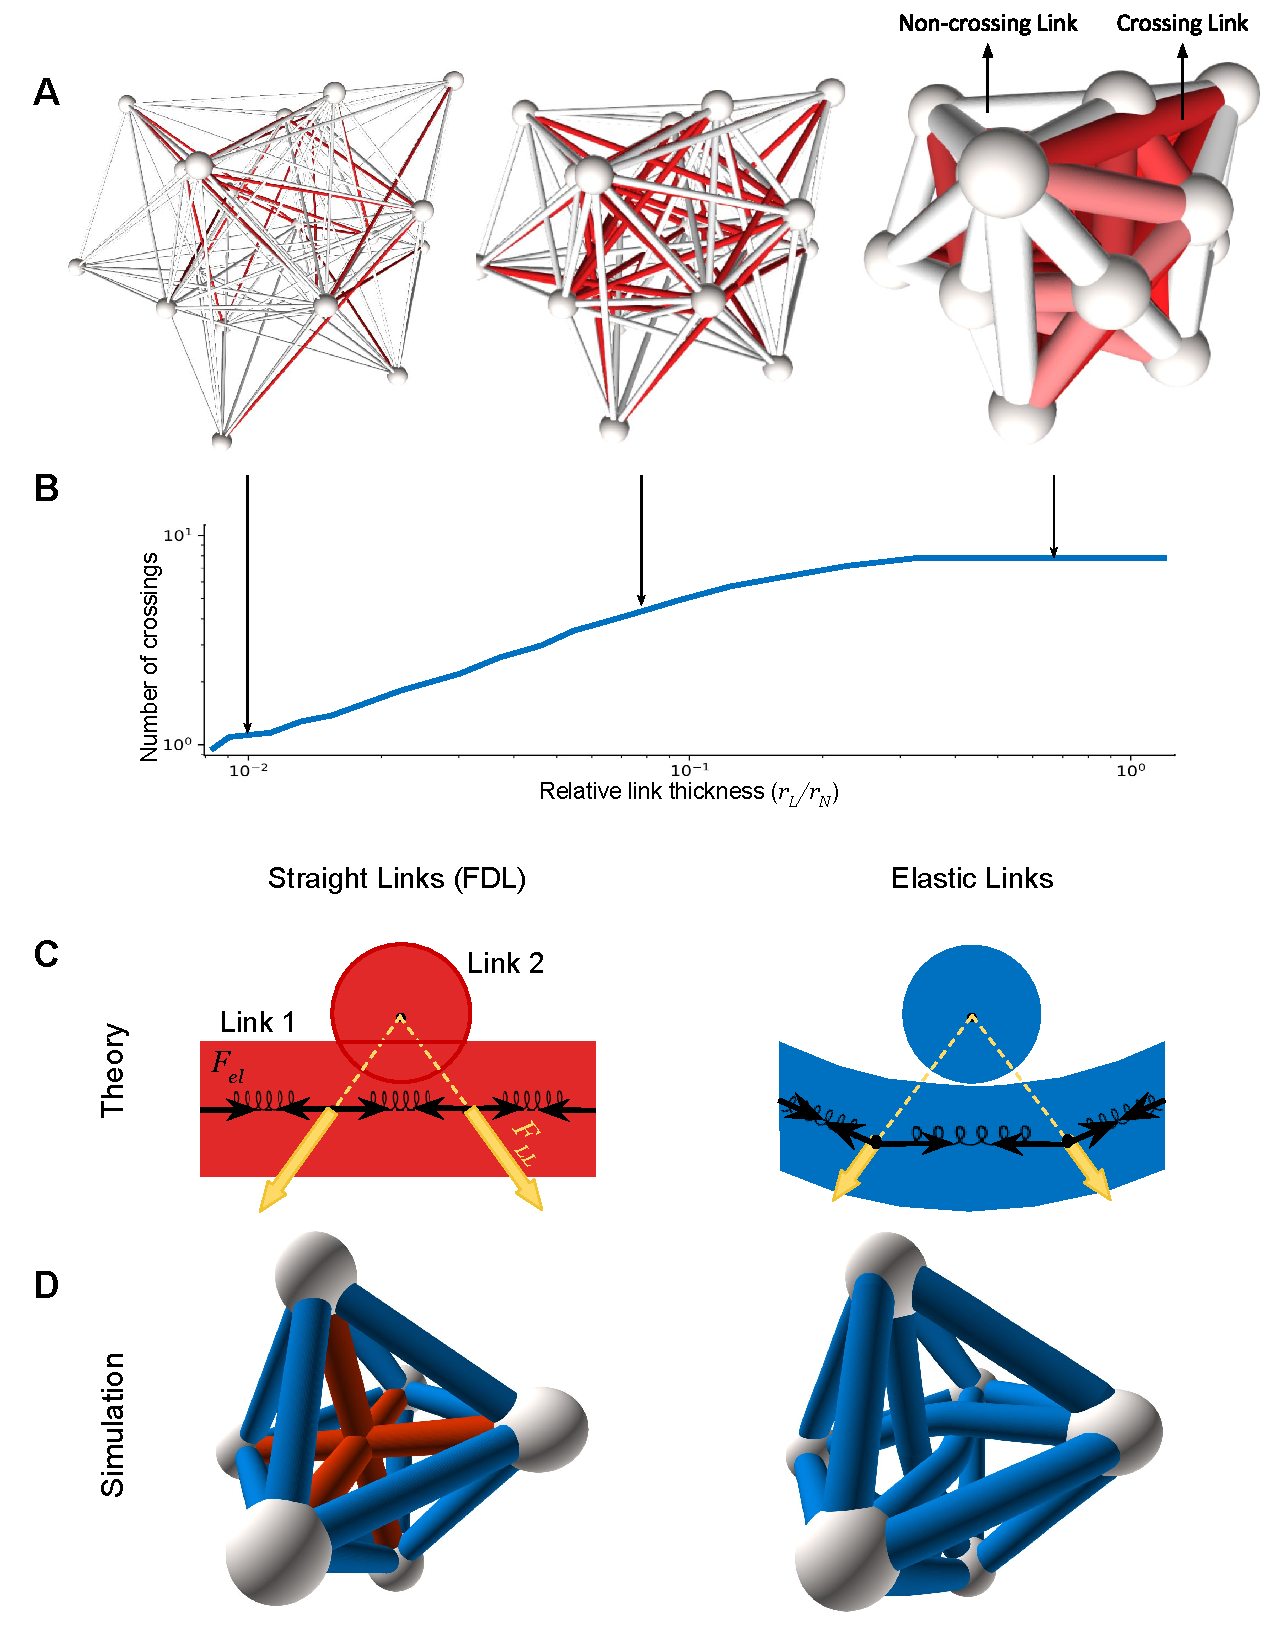
\includegraphics[width=.9\columnwidth]{fig-09-19/crs-resolve-0517.pdf}
    % 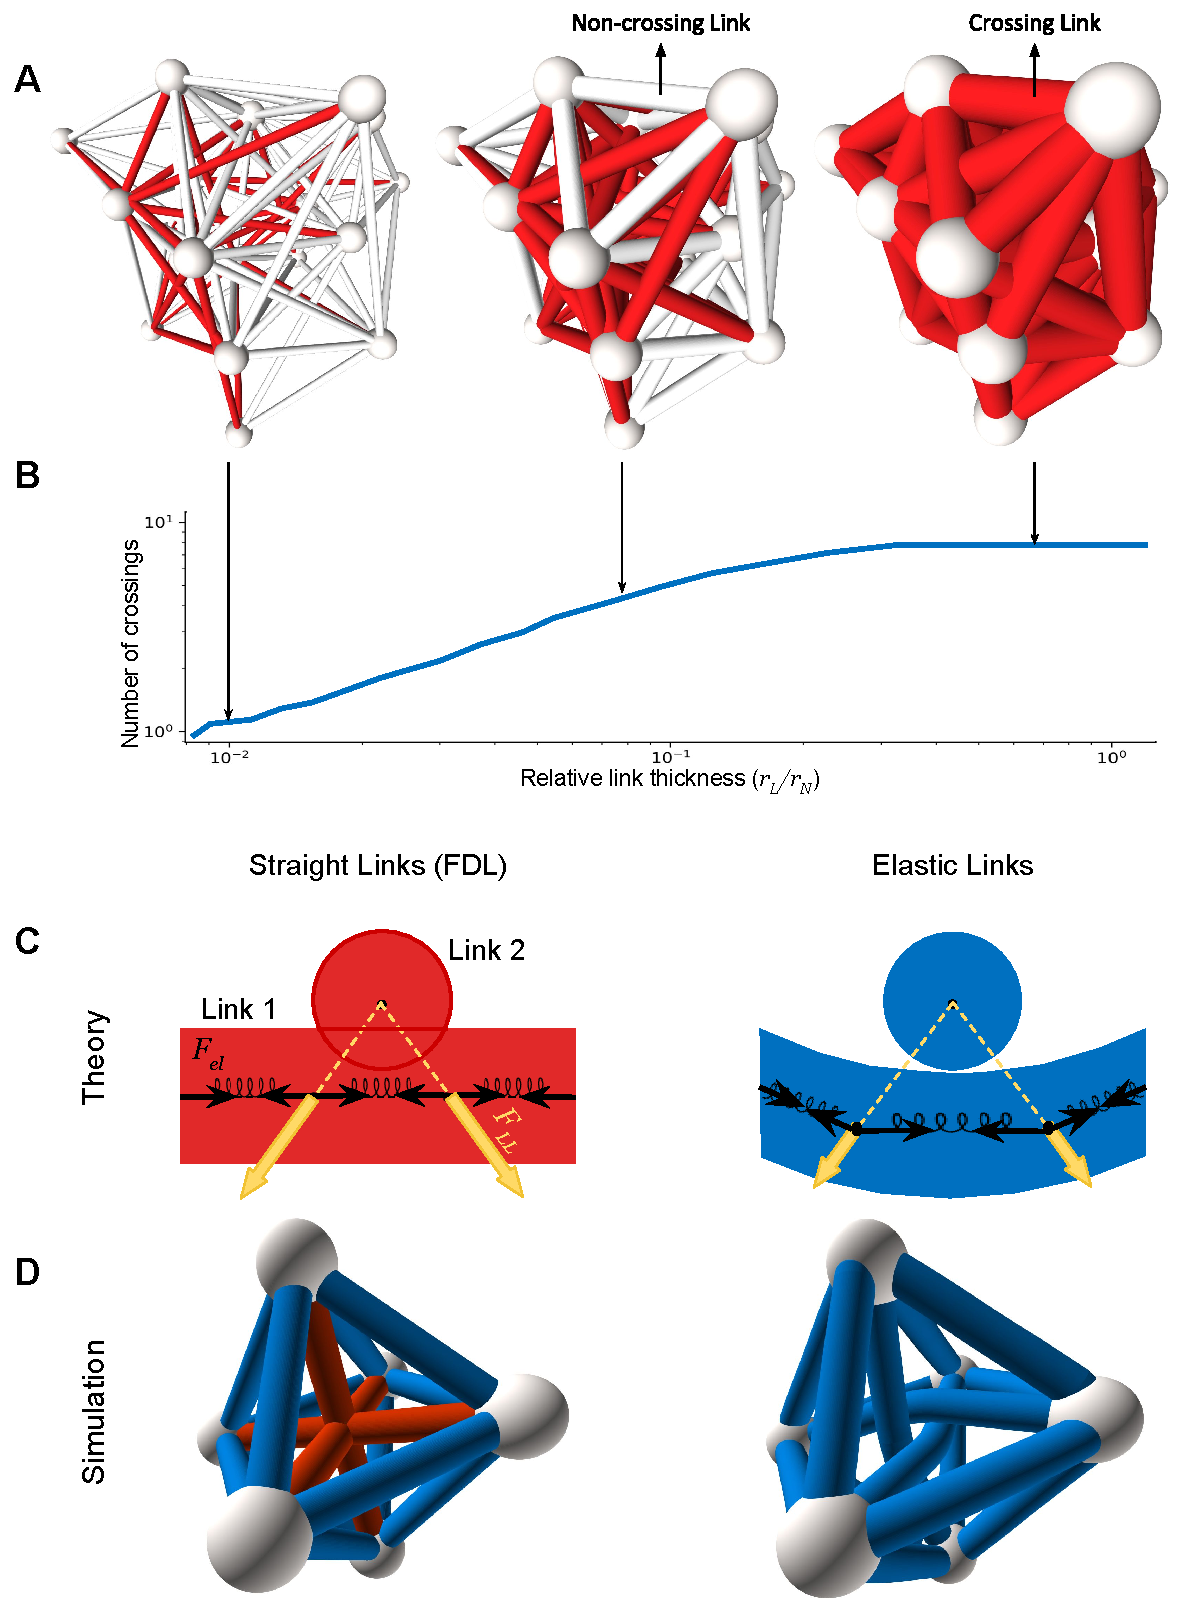
\includegraphics[width=.8\columnwidth]{fig-09-19/crs-resolve-061717.pdf}
    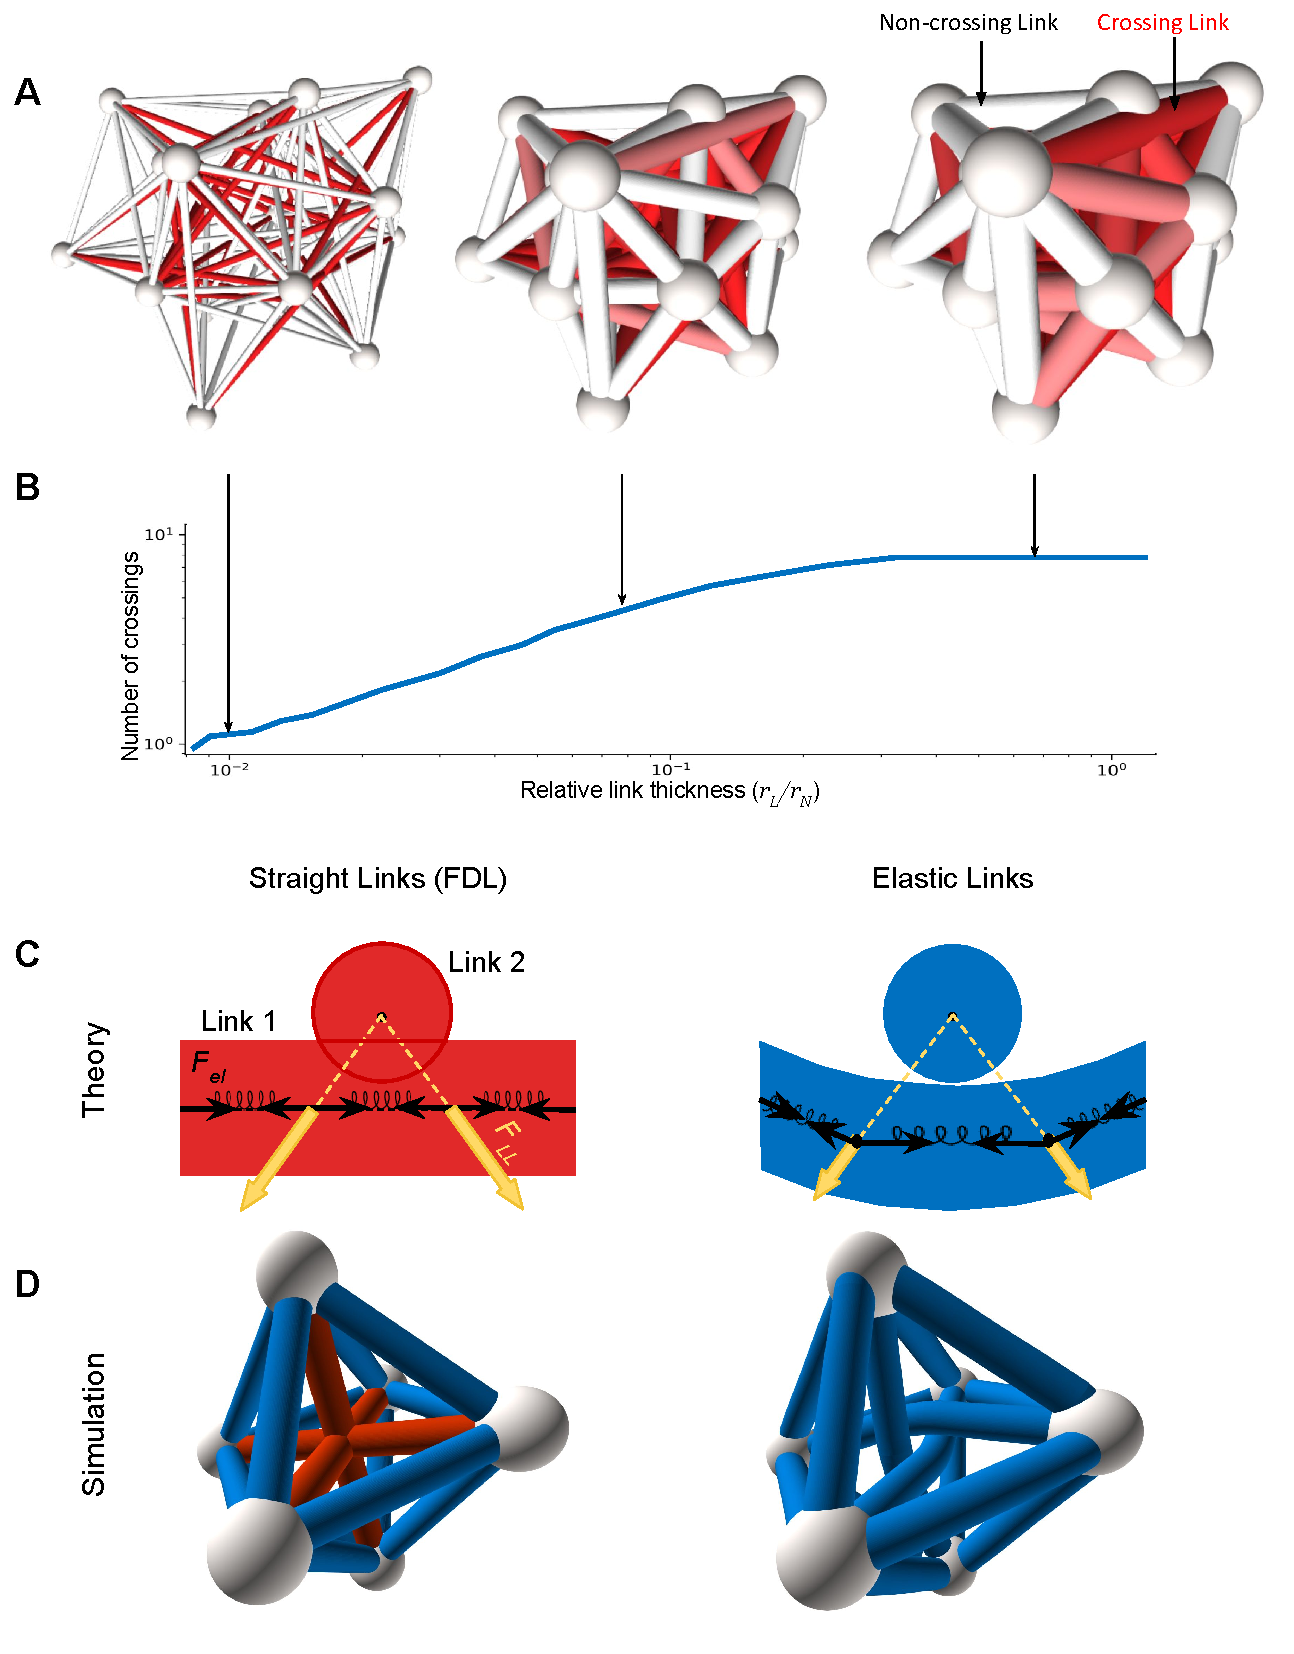
\includegraphics[width=.8\columnwidth]{fig-09-19/crs-resolve-071517.pdf}
    \caption{\scriptsize
    {\bf (A)}  Crossing links for a Barabasi-Albert (BA) network ($N = 20, m = 3$) in space, drawn by FDL. While increasing the link thickness $r_L$, the network occupies more space and crossings increase. 
    {\bf (B)} The plot shows the trend by which the number of crossings increases in a BA network with $N=100, m =3$ laid out in 3D using FDL.
    The number of crossings increases linearly with $r_L$ at first, before tapering off due to finiteness of the network. It can be shown (SI sec.\ref{ap:cross}) that layouts which result in random link orientations yield such linear trend in the growth of the number of crossings.
    {\bf(C) How ELI works:} We simulate the elastic links as a stretched, flexible rubber band, which can be thought of as many short springs connected to each other. 
    The elastic force $F_{el}$ of each spring is shown by black arrows.
    Links exert a repulsive force $F_{LL}$  on each other that falls sharply at radii larger than $r_L$. 
    First and second plot show how the ELI resolves crossing (red) links. {\bf(D)} shows a complete network with 6 nodes. Image on the left is laid out with FDL. The three red links all cross at the center. The right plot shows how the network looks after simulating ELI on it, after which the crossing is resolved. 
    }     
    \label{fig:crossings}
\end{figure}
\begin{figure}
    \vspace{4cm}
    \centering
    % 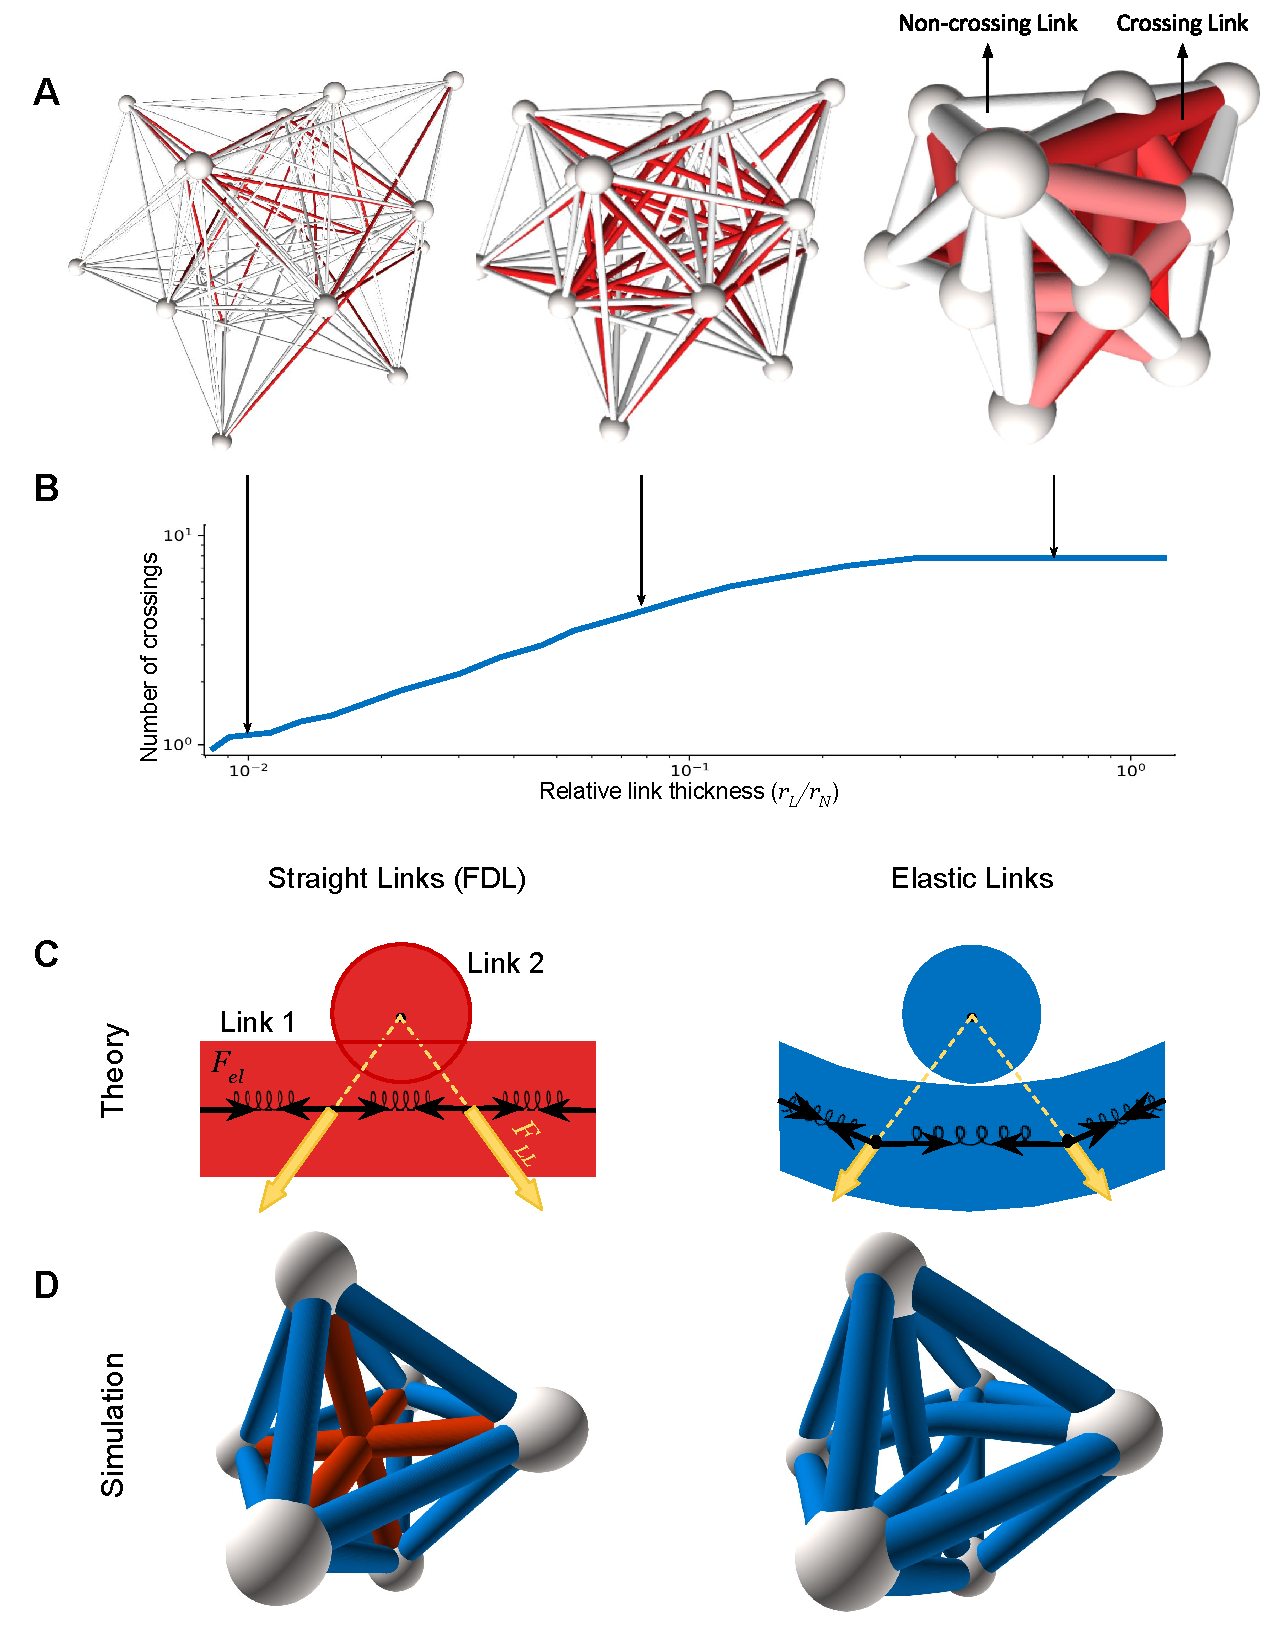
\includegraphics[width=.9\columnwidth]{fig-09-19/crs-resolve-0517.pdf}
    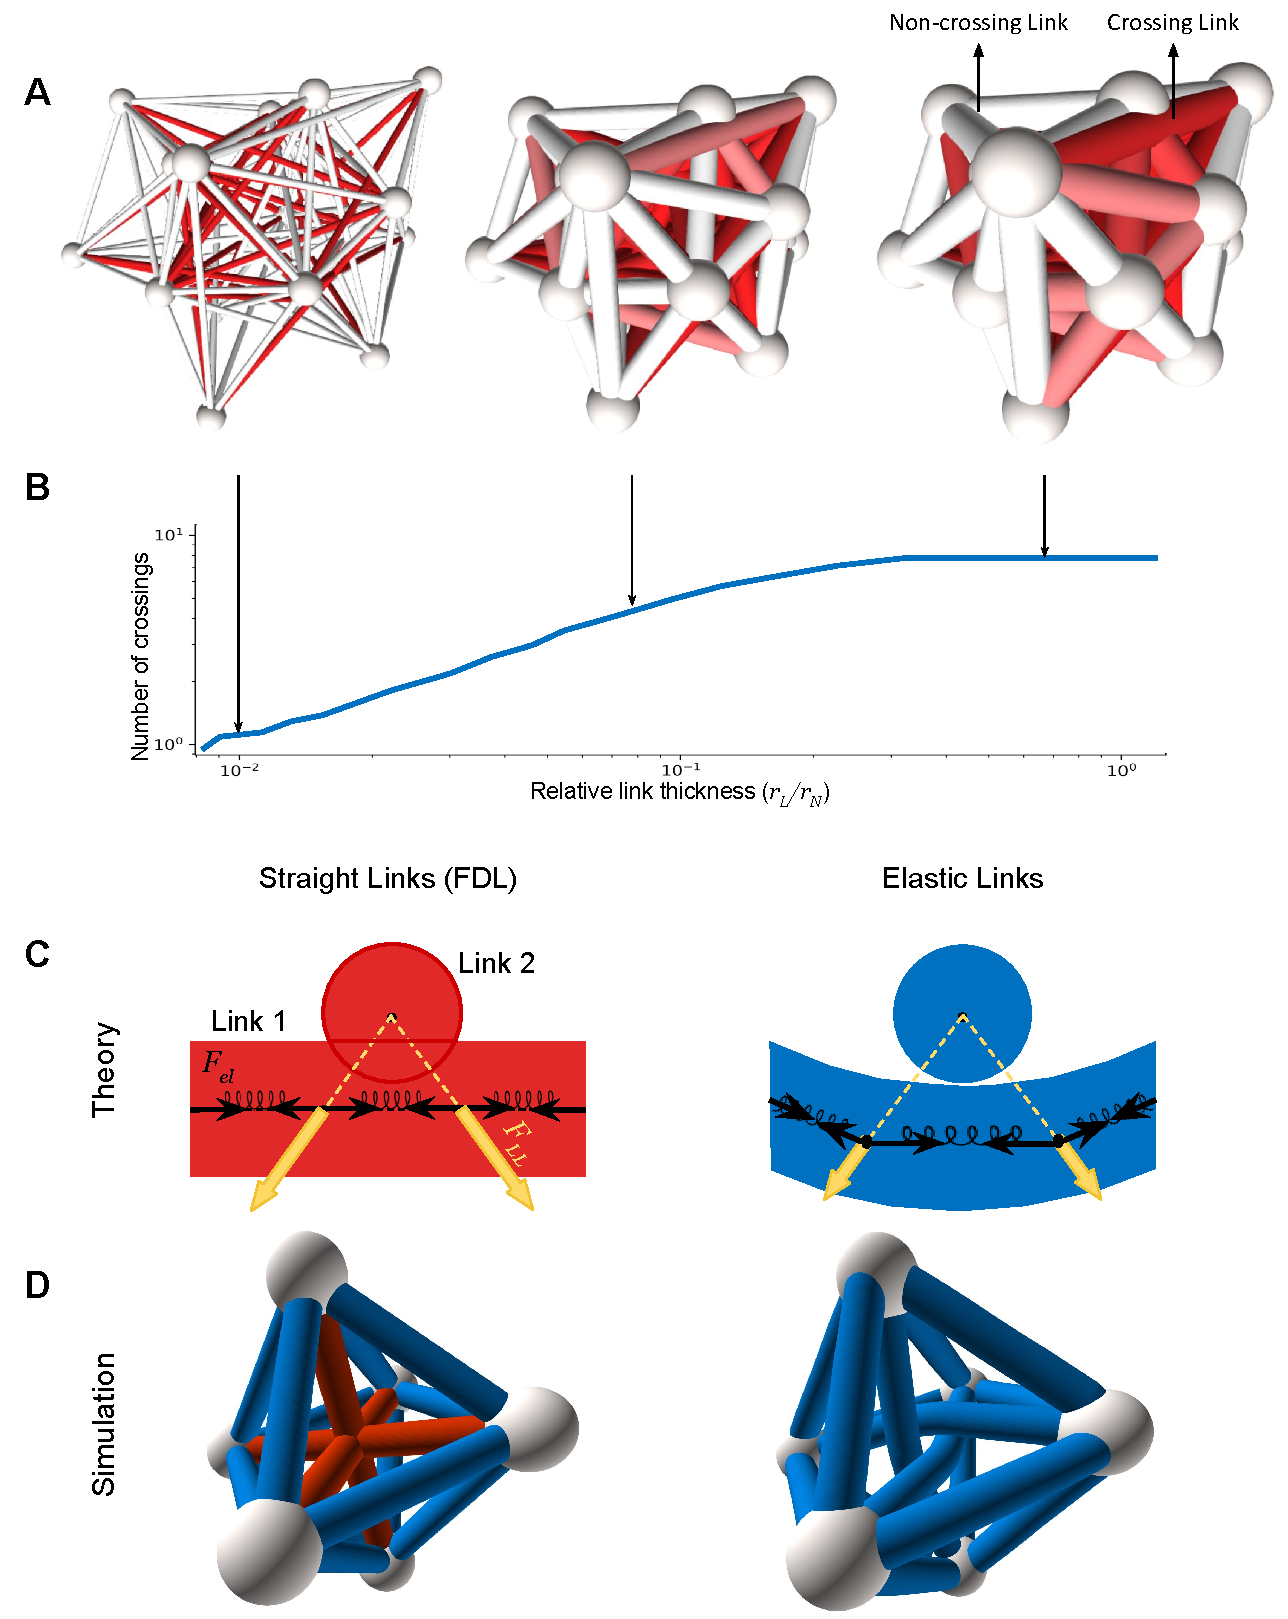
\includegraphics[width=.9\columnwidth]{fig-09-19/crs-resolve-0617.pdf}
    \caption{\scriptsize
    {\bf (A)}  Crossing links for a Barabasi-Albert (BA) network ($N = 20, m = 3$) in space, drawn by FDL. While increasing the link thickness $r_L$, the network occupies more space and crossings increase. 
    {\bf (B)} The plot shows the trend by which the number of crossings increases in a BA network with $N=100, m =3$ laid out in 3D using FDL.
    The number of crossings increases linearly with $r_L$ at first, before tapering off due to finiteness of the network. It can be shown (SI sec.\ref{ap:cross}) that layouts which result in random link orientations yield such linear trend in the growth of the number of crossings.
    {\bf(C) How ELI works:} We simulate the elastic links as a stretched, flexible rubber band, which can be thought of as many short springs connected to each other. 
    The elastic force $F_{el}$ of each spring is shown by black arrows.
    Links exert a repulsive force $F_{LL}$  on each other that falls sharply at radii larger than $r_L$. 
    First and second plot show how the ELI resolves crossing (red) links. {\bf(D)} shows a complete network with 6 nodes. Image on the left is laid out with FDL. The three red links all cross at the center. The right plot shows how the network looks after simulating ELI on it, after which the crossing is resolved. 
    }     
    \label{fig:crossings}
\end{figure}
} %%% out
To accurately lay out 
%\footnote{Optimal in terms of wiring length. 
%If other constraints are the primary concern, other methods should be used.} 
physical networks, we aim to arrange the links and the nodes in such a way that the total link length is minimized for a fixed $r_L$. 
This requires us to find the shortest path each link must follow, even when the optimal straight path is obstructed by other nodes and links, a problem similar to stretching a flexible rubber band between a series of obstacles (see \cite{novikov1984}, and SI sec.\ref{ap:affine} for proof). To achieve this we build a model in which each force in the network is determined by the gradient of the total potential energy,  
\begin{align}
    V &= V_{el} + V_{NL} +V_{NN} + V_{LL} \cr 
    &= {k\over 2}\sum_l\int ds_l \left|{d\vec{x}_l\over ds_l} \right|^2 + 
    \left. k\sum_{i=1}^N  \sum_{l\in <i>}  \vec{X}_i \cdot{d\vec{x}_l%\pr{l^{(\mathrm{end})}_l} 
    \over ds_l}\right|_{s_l = s_l^{(\mathrm{end})}}
    \cr
    &+ A_N\sum_{i\ne j}  \exp\left[- {|\vec{X}_i-\vec{X}_j|^2 \over 4r_N^2}\right]+A_L\sum_{l\ne m} \iint ds_lds_m 
    \exp\left[- {|\vec{x}_l-\vec{x}_m|^2 \over 4 r_L^2}\right] ,
 \label{eq:Vfull}
\end{align}
where $V_{el}$ represents the total elastic potential $E_l$ of all links $l=1,...,L$, where each link is an elastic cylinder with radius $r_L$ and links experience both an internal elastic force and short-range external repulsive force from other links and nodes; $V_{NL}$ captures the node-link interactions at link endpoints. Nodes and links are unable to cross each other's boundaries, a constraint ensured by a short-range repulsive force in
$V_{NN}$  (node-node interaction)  and  $V_{LL}$ (link-link interaction) modeled as short-range Gaussian potentials whose strength is set by $A_N$ and $A_L$
% \footnote{Other potentials of the form $\exp[-|\vec{X}_i-\vec{X}_j|^n/(2r)^n]$ with $n>2$ may also be used. The higher the $n$, the steeper will be the potential.}
(SI sec.\ref{ap:repel}). 
%The potential energy depends on the elastic constant, $k$, 
In \eqref{eq:Vfull} $s_l$ is the length parameter of link $l$ and  $\vec{x}_l(s_l,t)$ represents the position of a point along the center of the link at time $t$;
$s_l^\mathrm{(end)}$ is the parameter value at the endpoints of link $l$;
$l\in <i>$ represents the set of links connected to node $i$; 
$\vec{X}_i(t)$ is the position of node $i$; $r_N$ is the range of the node-node repulsive force; $k$ is the elastic constant of the links.
The link potentials are defined for infinitesimal link segments of length $ds_l$ and are integrated over the links to yield the full potential energy of the network. 
In the dense phase the lowest energy solution of \eqref{eq:Vfull} can lead to sharp bending of some links, which is avoided by using a Gay-Berne \cite{gay1981modification,berne1972gaussian} potential employed in polymer physics \citep{everaers2003interaction,babadi2006coarse,mergell2003modeling,cleaver1996extension} adapted to elastic links (SI sec.\ref{ap:ell}).


To allow the system to relax to a low energy state and avoid oscillatory behavior, we assume that the network is embedded in a high viscosity medium. 
Therefore, the position of the nodes and links follow first order gradient descent equations of motion towards a minimum of the potential energy
\begin{align}
    \lambda_N {dX_i\over dt} &= -{\ro V \over \ro X_i} %- \vec{\del}_{\vec{X}_i} \left[V_{\mathrm{NL}} + V_{NN} \right]
    \label{eq:nodes}\\
    \lambda_L {dx_l \over dt} & =  -{\ro V \over \ro x_l} + {d\over ds_l} {\ro V \over \ro (dx_l /ds_l)}   \label{eq:Langevin0},
\end{align}
where $\lambda_N$ and $\lambda_L$ are the node and link friction constants (SI sec.\ref{ap:eom}). 
We begin by using FDL to fix the initial node positions. 
We call the $\lambda_N\to \infty$ limit, where the node positions are fixed, and thus only the links can reorganize themselves, the Elastic Link Model (ELI).
For finite $\lambda_N \sim \lambda_L$, both nodes and links are free to move, yielding the Fully Elastic Link Model (FUEL). 
To obtain the optimal layout, we run  \eqref{eq:nodes}--\eqref{eq:Langevin0} until the forces on the right 
vanish, obtaining the equilibrium state corresponding to a minimum of \eqref{eq:Vfull}.
Equations \eqref{eq:Vfull}--\eqref{eq:Langevin0} represent a special case of general manifold dynamics, used to model polymer dynamics \cite{mezard1991replica}. 
The network has an uneven potential energy landscape \cite{parisi2002physical} with a multitude of local minima
%\footnote{In the space of all possible configurations of the paths the links take.
%If we approximate links as a collection discrete segments, this space will be finite dimensional, with dimensions equal to the number of segments. 
%For truly smooth links, this space is the space of all smooth paths and is ill-defined mathematically, for the same reason that path integrals are ill-defined.}, 
hence identifying the globally optimal configuration is NP hard (SI sec.\ref{ap:np}).
We therefore use simulated annealing \cite{hwang1988simulated} to approach an energetically favorable local minimum (SI sec.\ref{ap:np}). 
Fig. \ref{fig:crs-lat}E shows how FUEL finds the correct 3D configuration of a lattice, starting from a random layout. 
%Fig. \ref{fig:lattice}A  shows the time evolution of the total link length during the simulation, together with snapshots of the layout at each stage. 
The combination of noise and finiteness of the repulsive forces can be exploited to help %correctly exploiting discreteness of links allows 
the system get out of local minima by tunnelling through the finite potential walls and unwrap completely into the familiar 3D lattice layout (SI sec.\ref{ap:np}).
\outNim{ % 071917
\begin{figure}
    \centering
    % 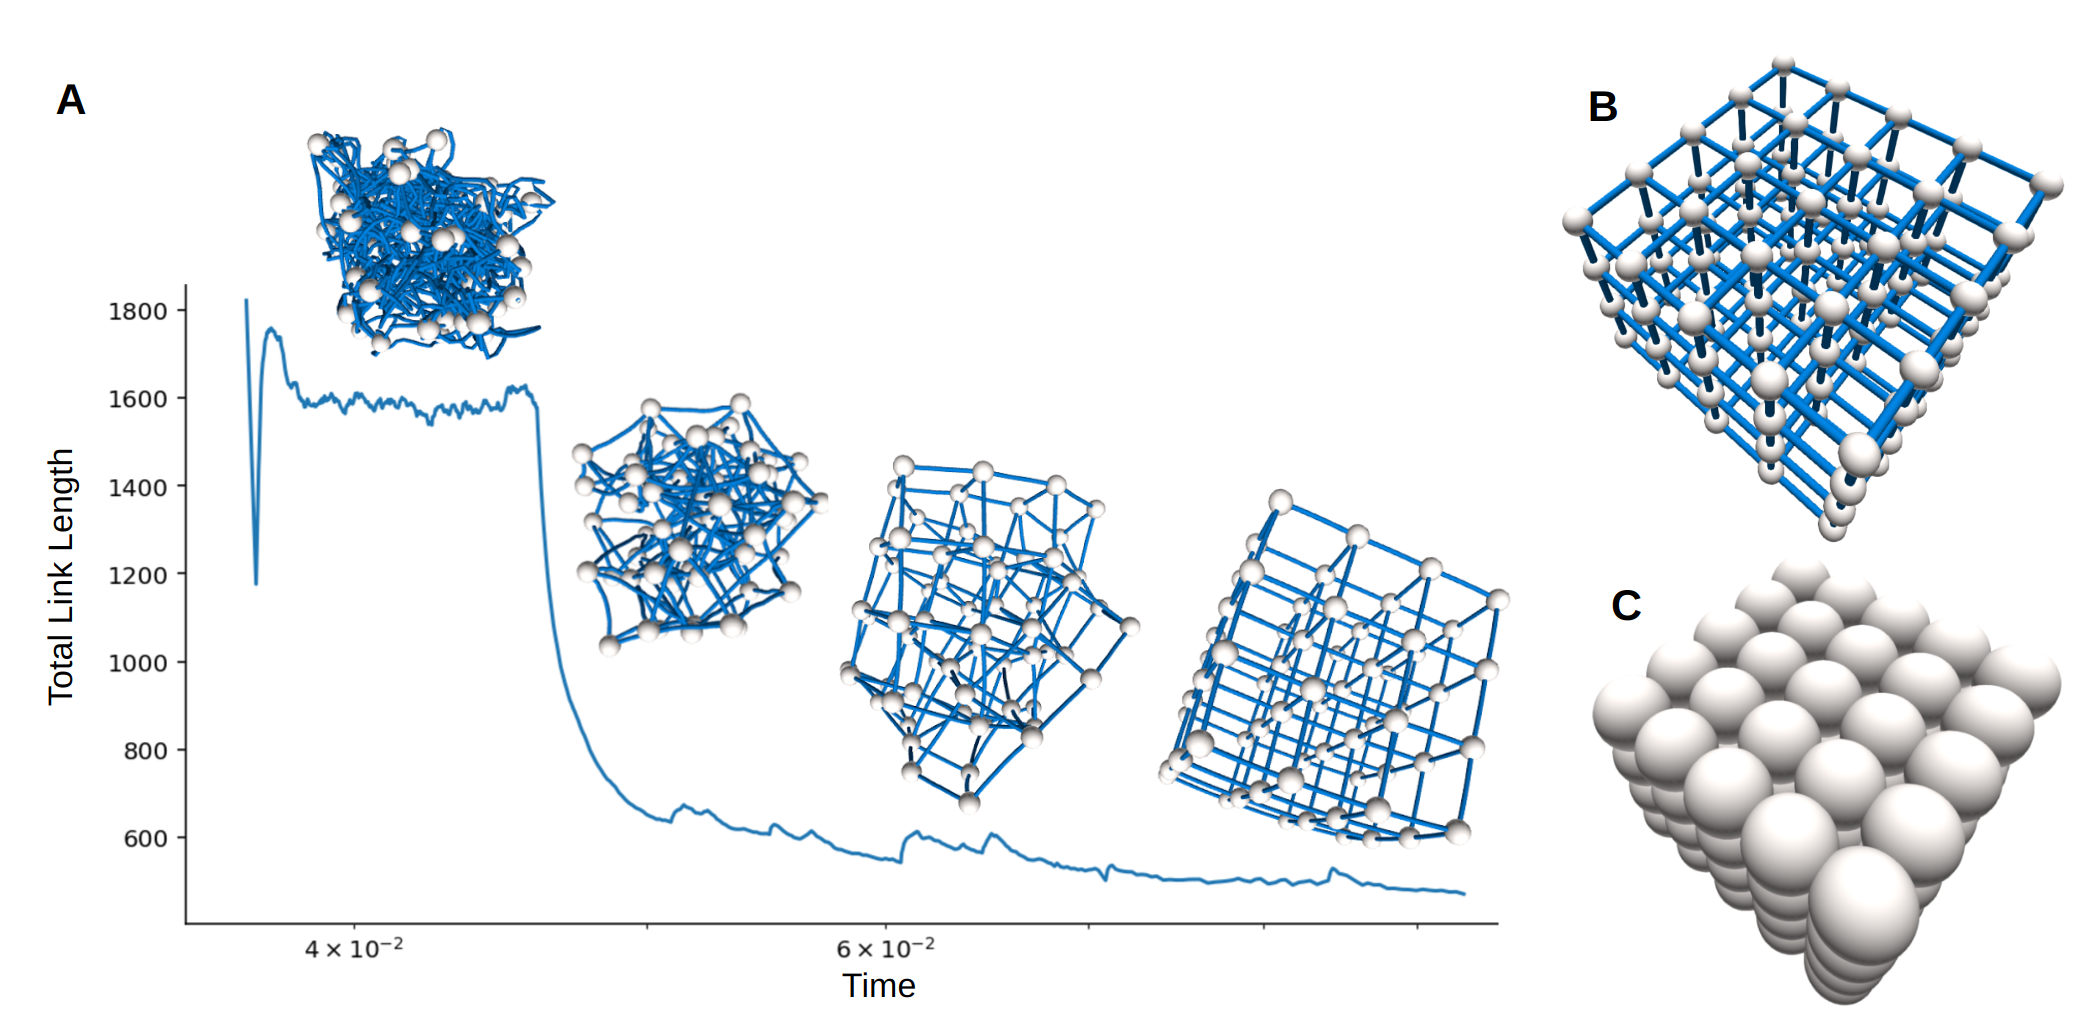
\includegraphics[width=\columnwidth]{fig-09-19/lattice-3.png}
    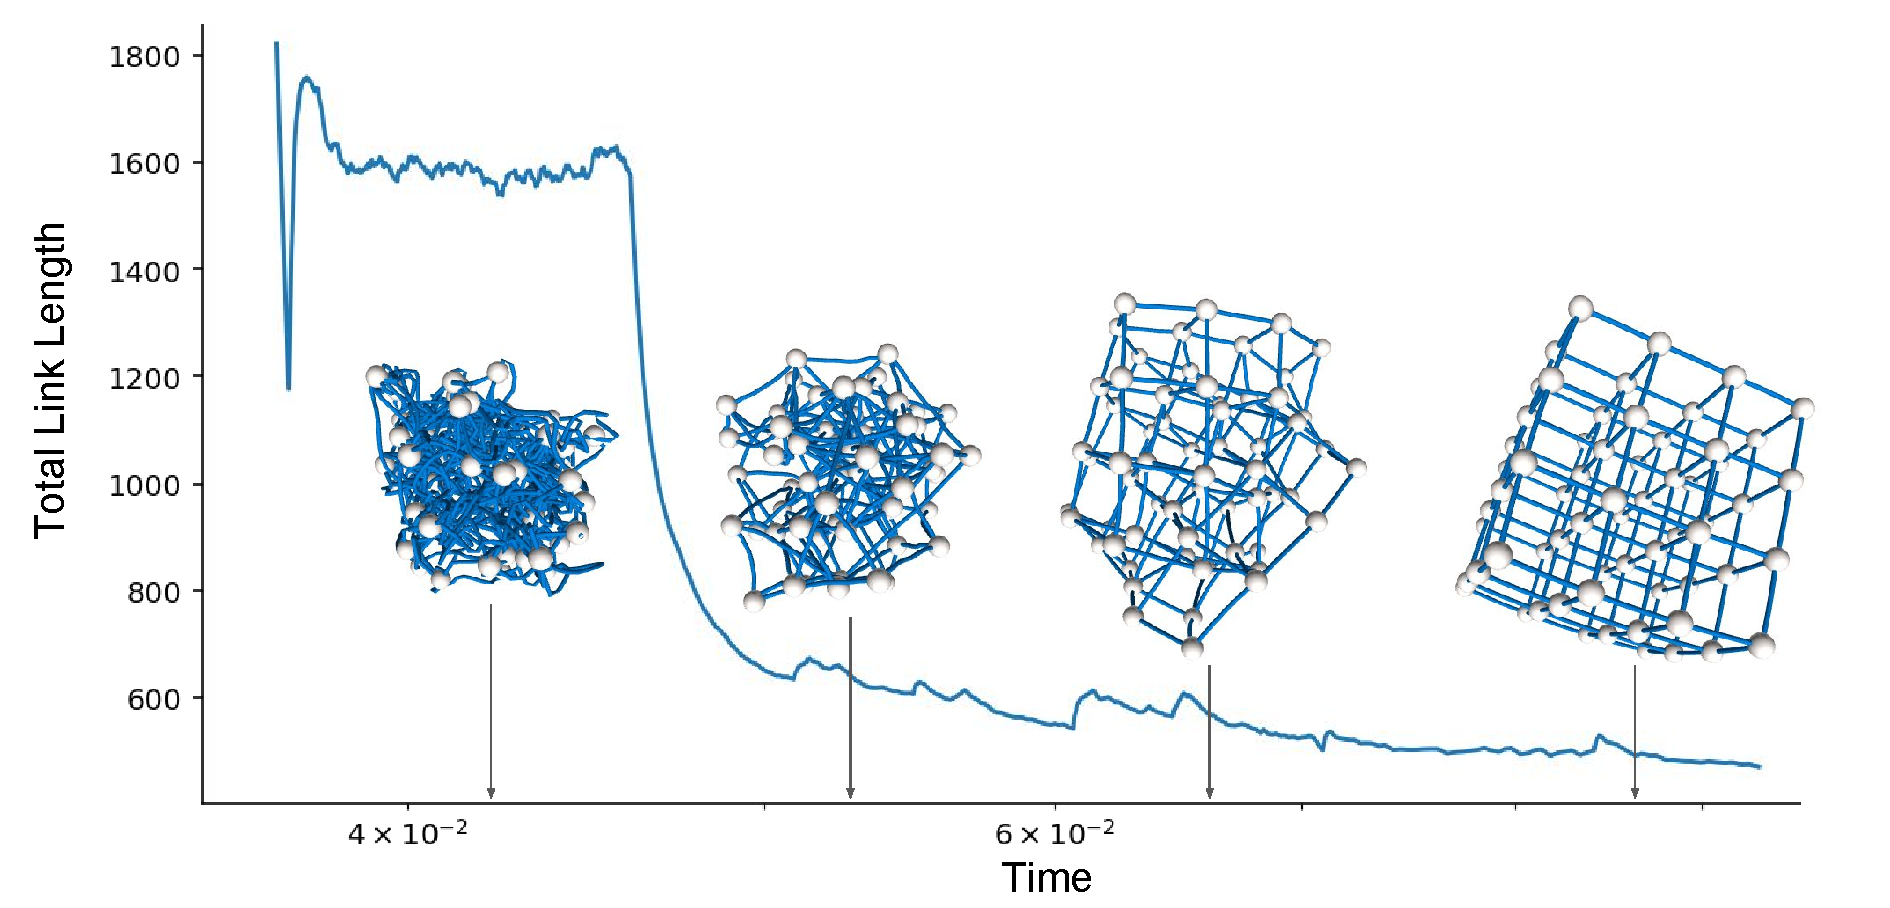
\includegraphics[width=\columnwidth]{fig-09-19/lattice-unwrap.pdf}
    \caption{\scriptsize %{\bf (A)}
    Simulation of the layout of a lattice with $r_L\ll r_N$. The link thickness corresponds to the actual thicknesses, while the node size is chosen based on proper visibility. Choosing short-range repulsion for nodes is crucial for getting a perfect lattice layout. Long range forces, e.g. electrostatic,  distort the layout at the boundaries. The plot shows the evolution of the total link length over time during the simulation, with several snapshots of the actual layout shown above each stage of the evolution. 
    The simulation started from a completely random layout. 
    We use simulated annealing to find the layout.
    Initially the thermal noise results in a very large total edge length, but it helps links pass through each other and thus resolve crossings.
    Still, in later stages the system is prone to get stuck in one of many local minima of the potential energy and not completely unfold. 
    To let the system unfold completely, we have exploited the discreteness and chose the number of link segments to be small. 
    This decreases the energy penalty of jumping from one local minimum to another and makes it more likely for the system to relax completely. 
    % {\bf (B)} A fully relaxed lattice, with actual node and link sizes. 
    % {\bf (C)} The same network if node size was set to the node repulsion radius $r_N$. 
    % When $r_L\ll r_N$, the push of nodes at $2r_N$ distance from each other determines the size of the layout. 
    % It is important to note that the node repulsion range $r_N$ is {\em not} the radius of nodes. The node radius may be chosen at any value smaller than $ r_N$. 
    %{\bf C}: The evolution of total link lengths as a function of time during the simulations. The first order dynamical equations \ref{eq:nodes} and \ref{eq:Langevin0} of E-ELM can lead to numerical instability if time steps are large. The inset shows that this numerical artifact is resolved by switching to smaller time steps.
    }
    \label{fig:lattice}
    \vspace{4cm}
\end{figure}
} %%%out
Fig. \ref{fig:phase-compare}A and %\ref{fig:phase-compare}
B show layouts generated using ELI (A) and FUEL (B), for a small %Barabasi-Albert (BA) 
network %with $N=10, m=3$
with different $r_L$, documenting a qualitative structural change as we increase $r_L$. 
While at small $r_L$ ELI and FUEL layouts are largely indistinguishable, for large $r_L$ there are visually apparent differences between them. 
Indeed, at small $r_L$ link crossings are rare and can be avoided by the local bending of the links. Consequently, 
the layouts of both ELI and FUEL are visually indistinguishable from FDL. 
As $r_L$ increases, links are increasingly unable to avoid each other by small local bendings and the FUEL layout starts to diverge from FDL-based layouts. We also start seeing considerable differences between ELI and FUEL. 
As the node positions are fixed in ELI, links are forced to follow long arcs outside the layout to reach their end nodes.
% \footnote{In FDL, the repulsive force between nodes is generally a long-ranged electrostatic force, falling as $F \propto r^{-2}$. 
% However, such long-range forces rarely exist in biological systems. Even in polymers, interactions are often modeled with the Lennard-Jones potential \cite{lennard1924determination}, which falls as $r^{-6}$ at large distances and like a hard-core interaction in very short distances.}
As the nodes can also move in FUEL, to avoid conflicts the links push the nodes away from each other. 
%The network avoids conflicts by pushing the nodes away from each other, creating space for the links. 

\begin{figure}
\centering
%\vspace{-2cm}
%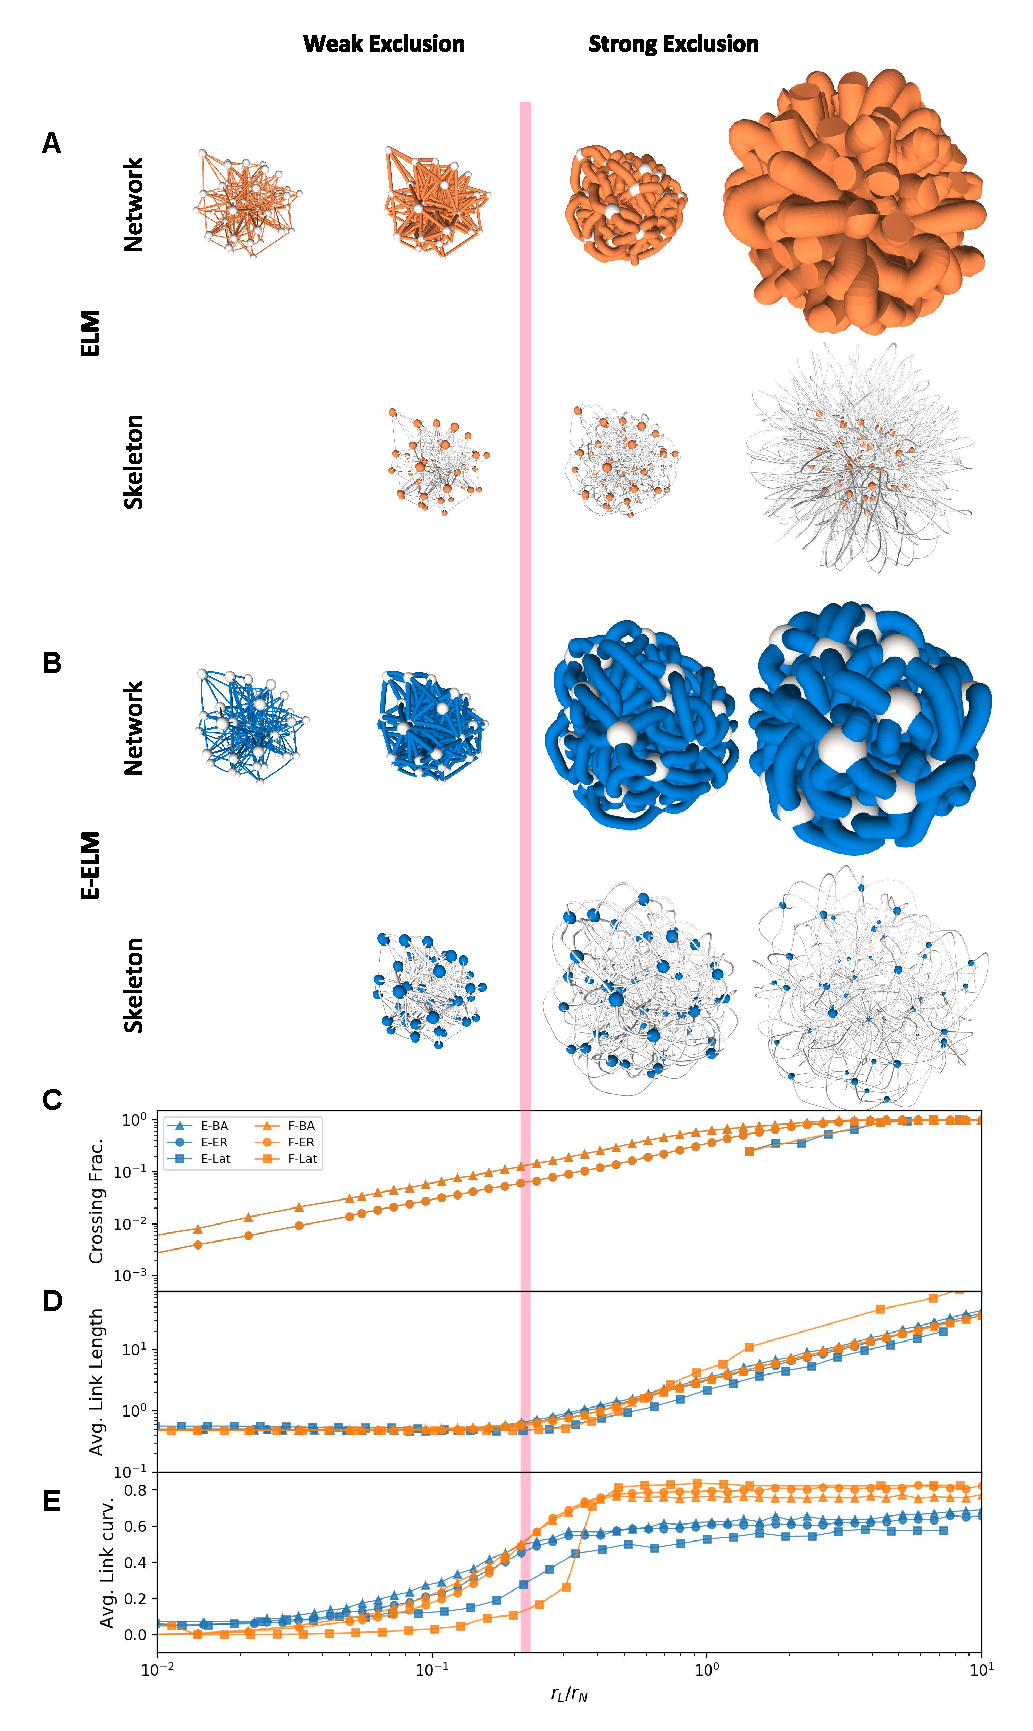
\includegraphics[width=.69\columnwidth]{fig-09-19/phase-051817.pdf}
% 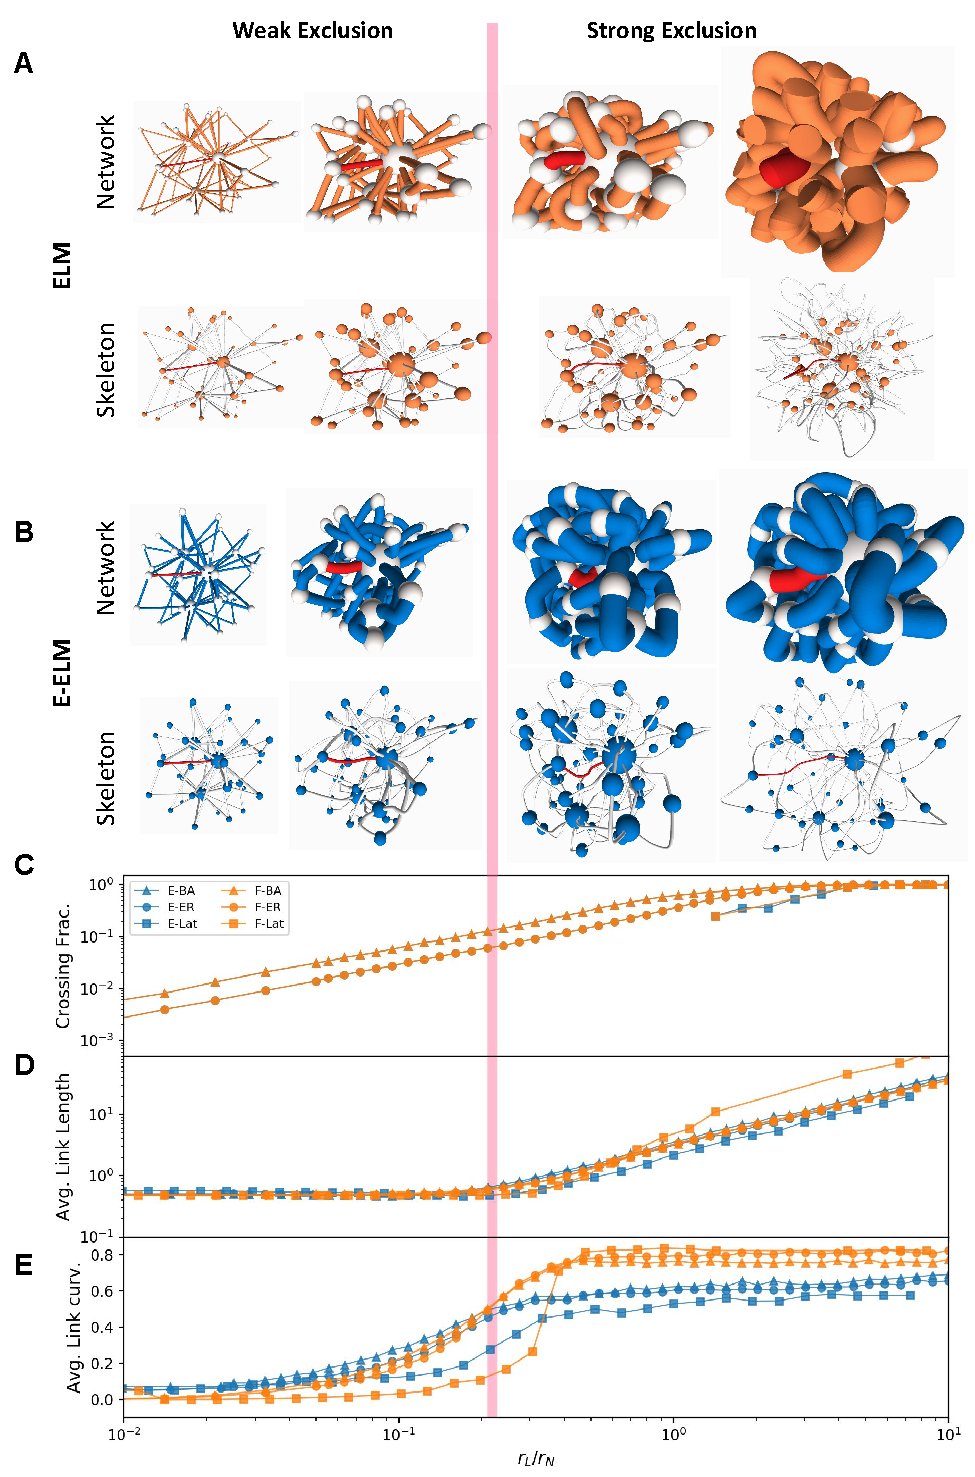
\includegraphics[width=.69\columnwidth]{fig-09-19/phase-061717.pdf}
% 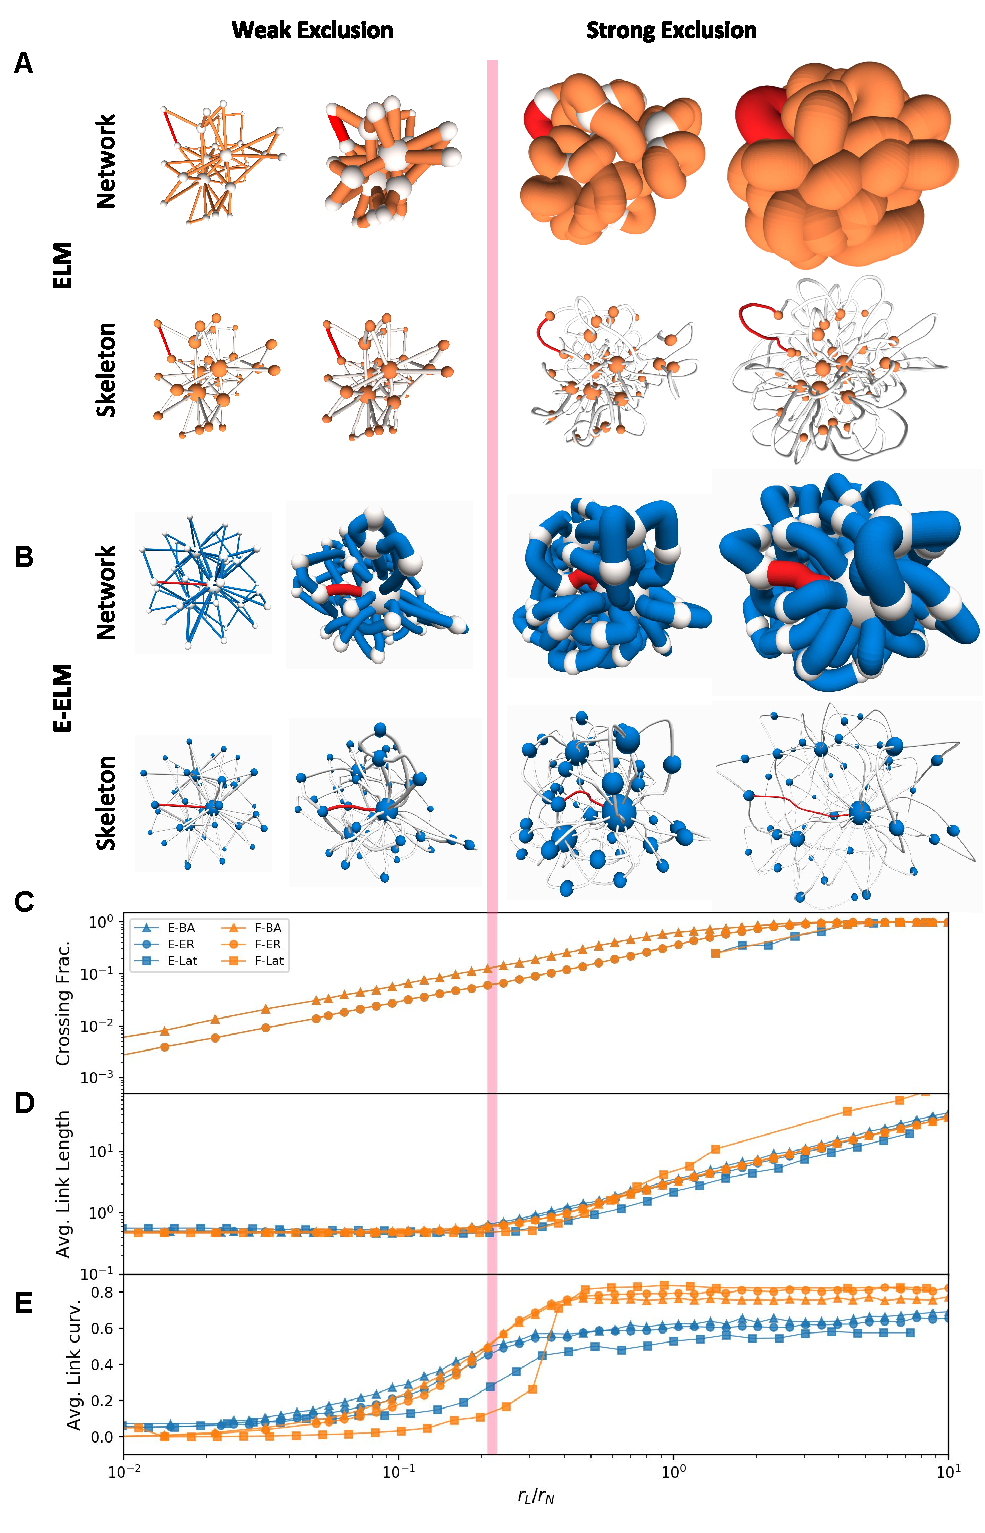
\includegraphics[width=.69\columnwidth]{fig-09-19/phase-071517.pdf}
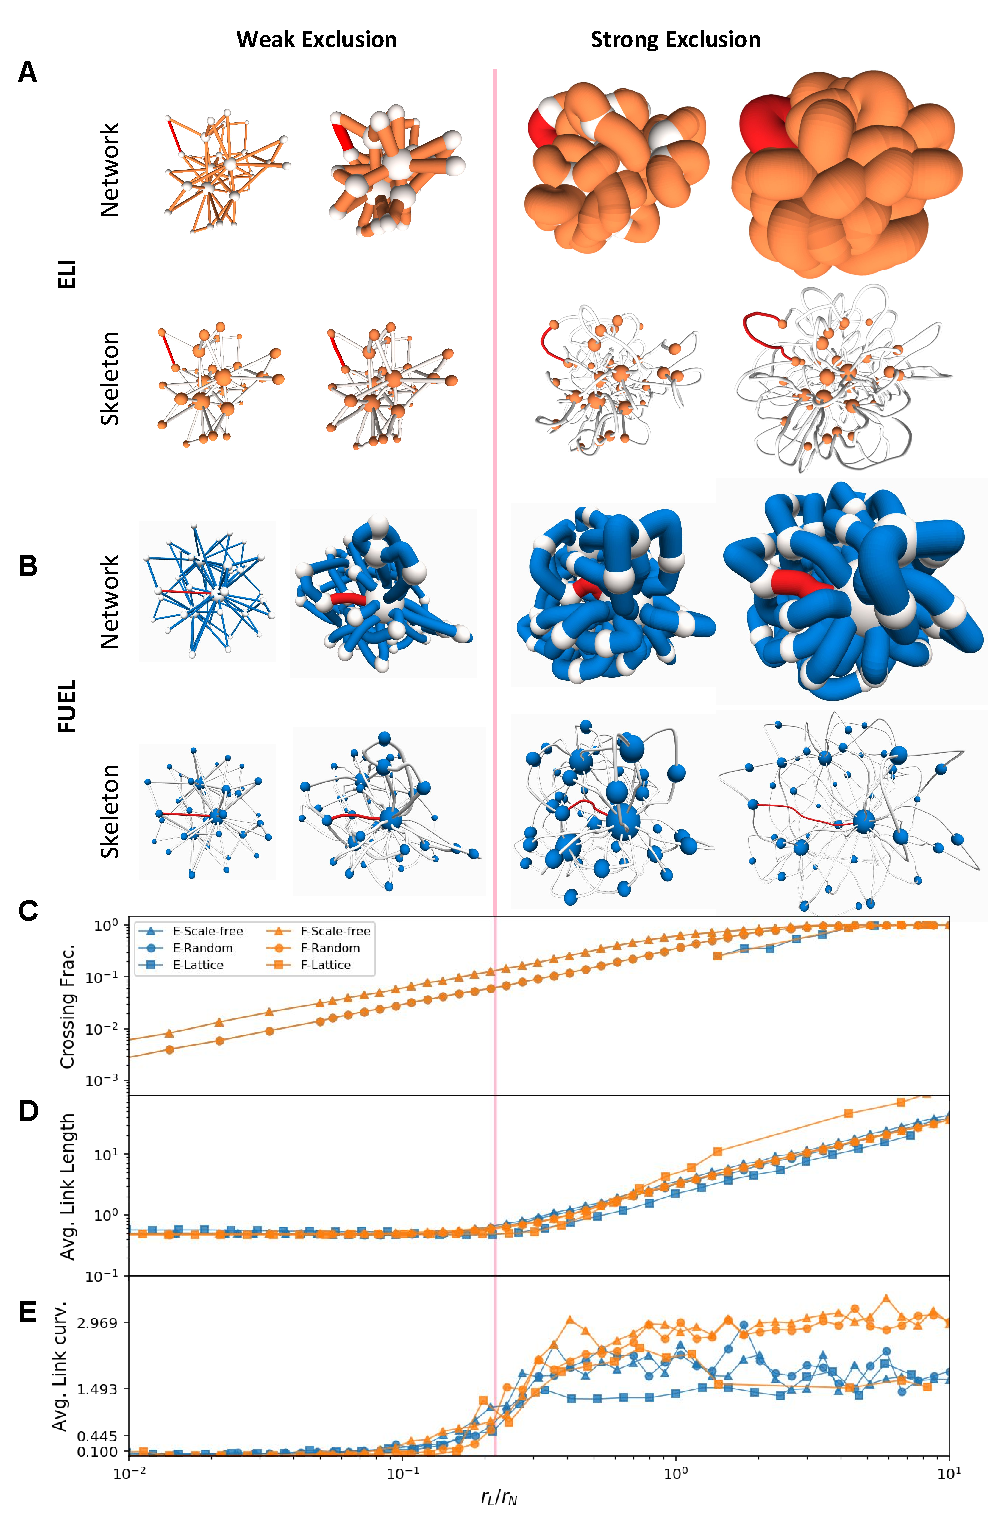
\includegraphics[width=.69\columnwidth]{fig-09-19/phase-full-071917.pdf}
\caption{%3D layouts  using ELM and E-ELM, and their phase diagram.
         \scriptsize {\bf ELI and FUEL at various link thicknesses:} ELI ({\bf A}, orange) and FUEL ({\bf B}, blue) used on a BA $N=10, m=3$. 
         Below each layout we show the skeleton, where the links are made thin, to show the paths of the links.
         ELI layouts were generated using the double-ellipsoidal metric, instead of Euclidean distance, to avoid links bending onto themselves in the strong exclusion phase. 
         At small thicknesses, $r_L \ll r_N$, both layouts are the similar to FDL. At larger $r_L$ in ELI links start bending to avoid each other. 
         At very large $r_L$, links don't fit inside the region containing the nodes and start making outward arcs. 
         FUEL at large $r_L$ behaves more gently and the layout size just grows linearly with the $r$.
         One link is highlighted as red to contrast the variation in link trajectories with increasing link thickness.
         {\bf Phases of ELI vs. FUEL:} {\bf (C)} 
         Orange and blue lines correspond to ELI (prefix ``F-'' in legend) and solid ones are FUEL (prefix ``E-'') layouts. Each symbol signifies a network topology: ER: Erdős-Renyi; BA: Barabasi-Albert; Lat: the 3D regular lattice.
         ({\bf D}) The average link length remains more or less constant in the weak exclusion regime (small $r_L/r_N$), but grows linearly in the strong exclusion regime for all three topologies and for both ELI and FUEL, unable to distinguish between topologies.  
         ({\bf E}) While total Link curvature of BA and ER overlap almost completely in both ELI and FUEL (bottom), the lattice does differ from them in the ELI. }    
    \label{fig:phase-compare}
\end{figure}

The transitions seen in Fig. \ref{fig:phase-compare}A,B with increasing $r_L$ also change the scaling properties of the layout. To show this, we first measure the average length of links $\be{l}$,
revealing a qualitative change in the behavior in $\be{l}$ (red strip Fig. \ref{fig:phase-compare}C, D, E) at a critical value for $r_L/r_N$:  at low $r_L$, the average link length $\be{l}$ remains unchanged despite orders of magnitude change in $r_L$.
This is particularly surprising, given that the number of potential crossings goes up ten fold (Fig. \ref{fig:phase-compare}C). 
The unchanged $\be{l}$ indicates that in this {\em weak exclusion regime} the layout avoids the increasing number of conflicts by local bending, without significantly altering the total link lengths. 
Once, however, $r_L$ exceeds a critical value, $\be{l}$ changes its behavior and increases linearly with $r_L$. 
In this {\em strong exclusion phase} local bending cannot resolve the conflicts any longer, forcing the links to drastically increase their length. 
In ELI, where the node positions are fixed, the links can only reach their nodes by taking long convoluted routes outside the network. 
In FUEL the links push the nodes away from each other. 
%In E-ELM, link crossings are avoided by pushing the nodes apart from each other. 
What is remarkable, however, is that despite the different mechanisms the two models employ, and the visually striking differences in the obtained layouts, the scaling of $\be{l}$ is largely indistinguishable in the two models.
  

We can estimate the critical $r_L$, thereby obtaining an insight into the origin of the observed transition. 
When the links are much thinner than the node repulsion range  $r_N$ the layout is determined by the repulsive forces between the nodes. 
Hence, the radius $R$ of the ``bounding sphere,'' representing the smallest sphere engulfing all nodes, is determined by the volume of $N$ loosely placed spheres of radius $r_N$, i.e. $ R^3 \sim Nr_N^3 $ (Fig. \ref{fig:trans}A). 
When the total volume of the links cannot fit any longer inside the sphere determined by the node positions, the layout must change. 
In this case the layout will be  dominated by the total link volume, and the cross sectional area of the layout $\pi R^2$ becomes comparable to the cross section of all links $ L r_L^2 \sim R^2$, where $L$ is the number of links (Fig. \ref{fig:trans}B). 
\begin{figure}
    \centering
    % 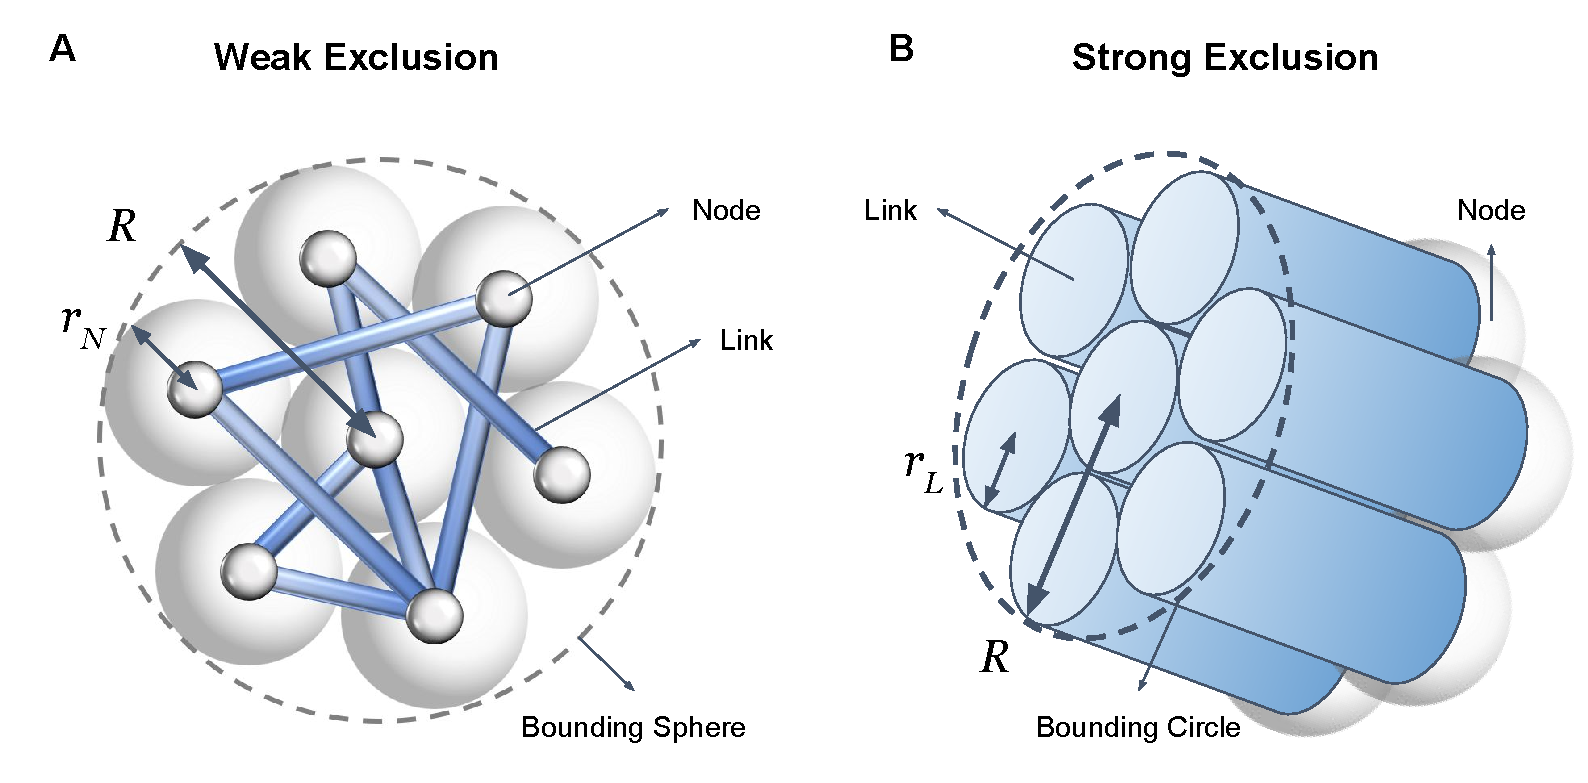
\includegraphics[width=\columnwidth]{fig-09-19/transition.pdf}
    %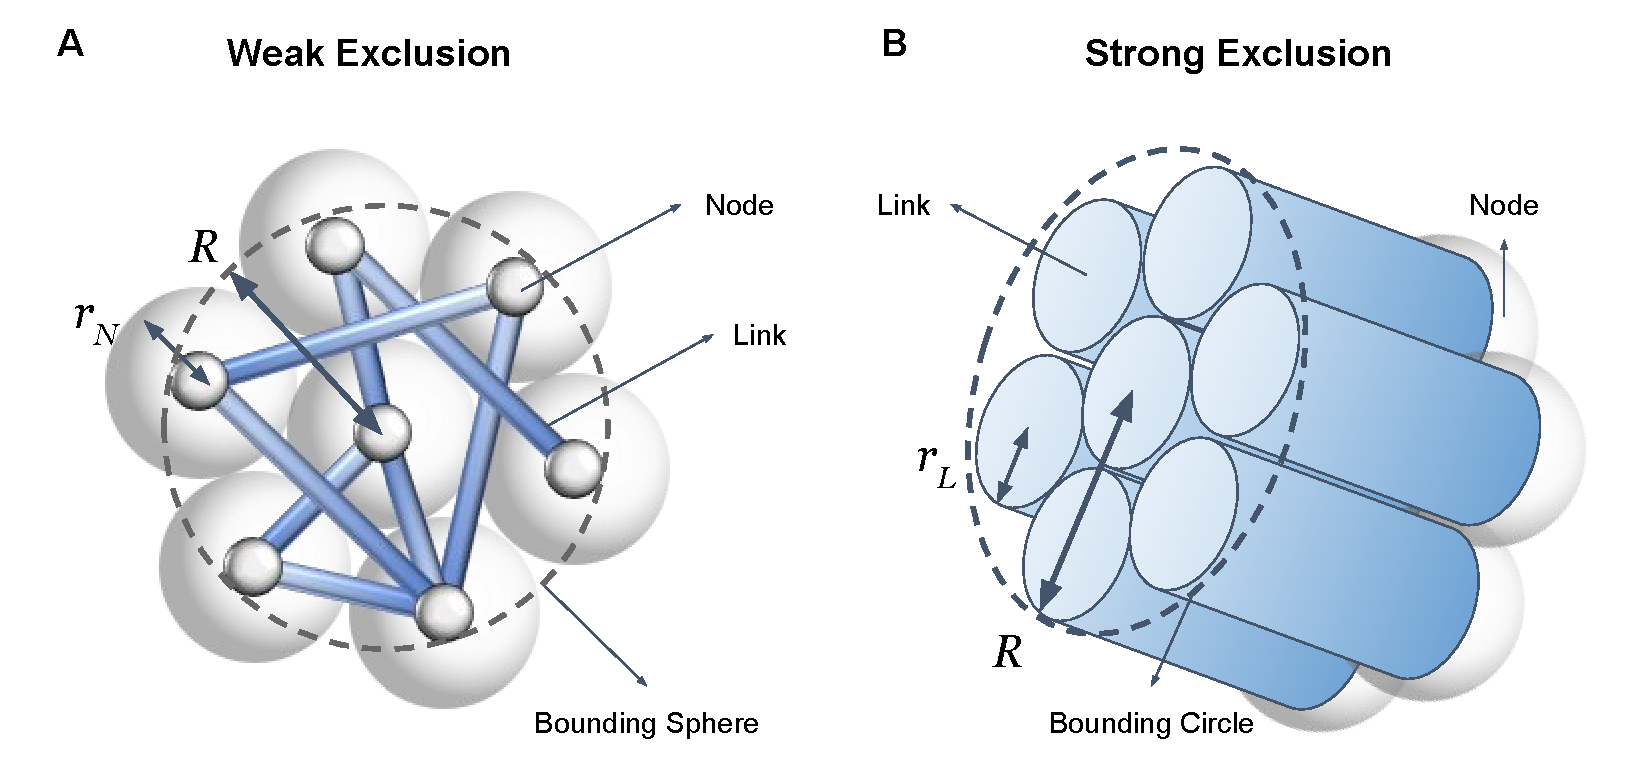
\includegraphics[width=\columnwidth]{fig-09-19/trans-2.pdf}
    %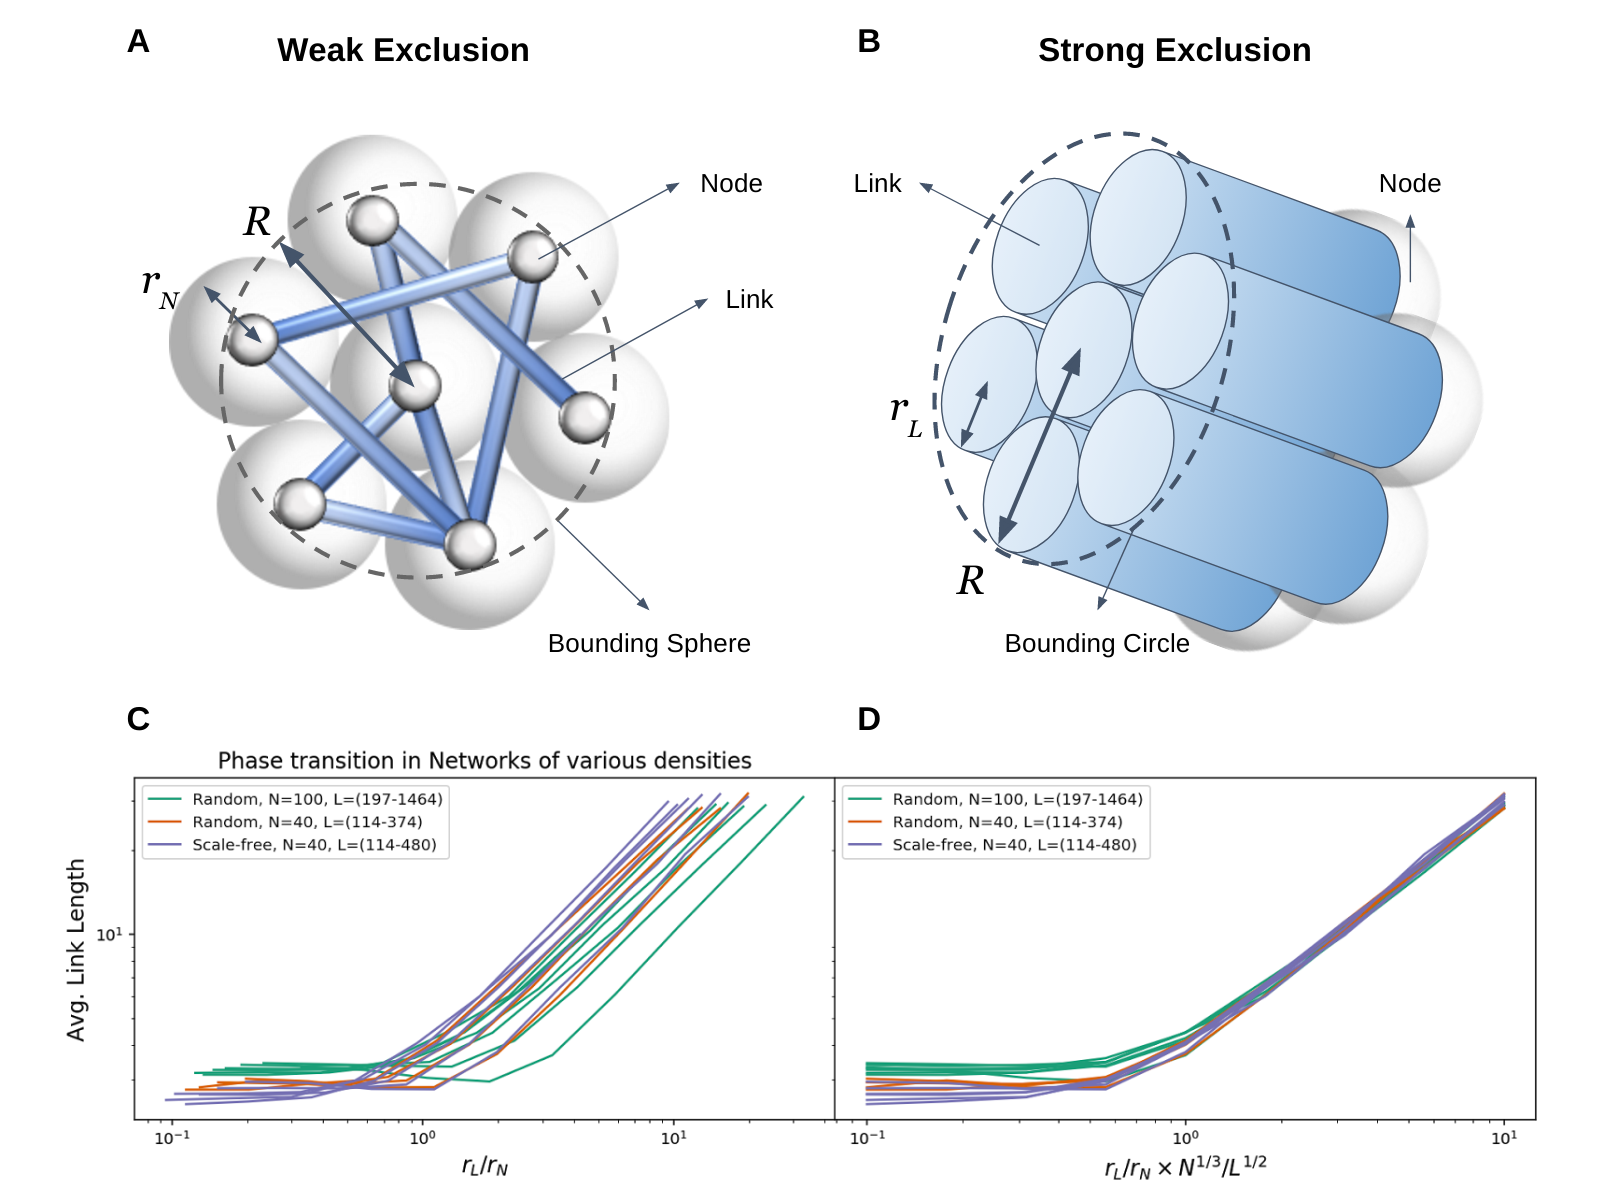
\includegraphics[width=\columnwidth]{fig-09-19/transition-2.png}
    % 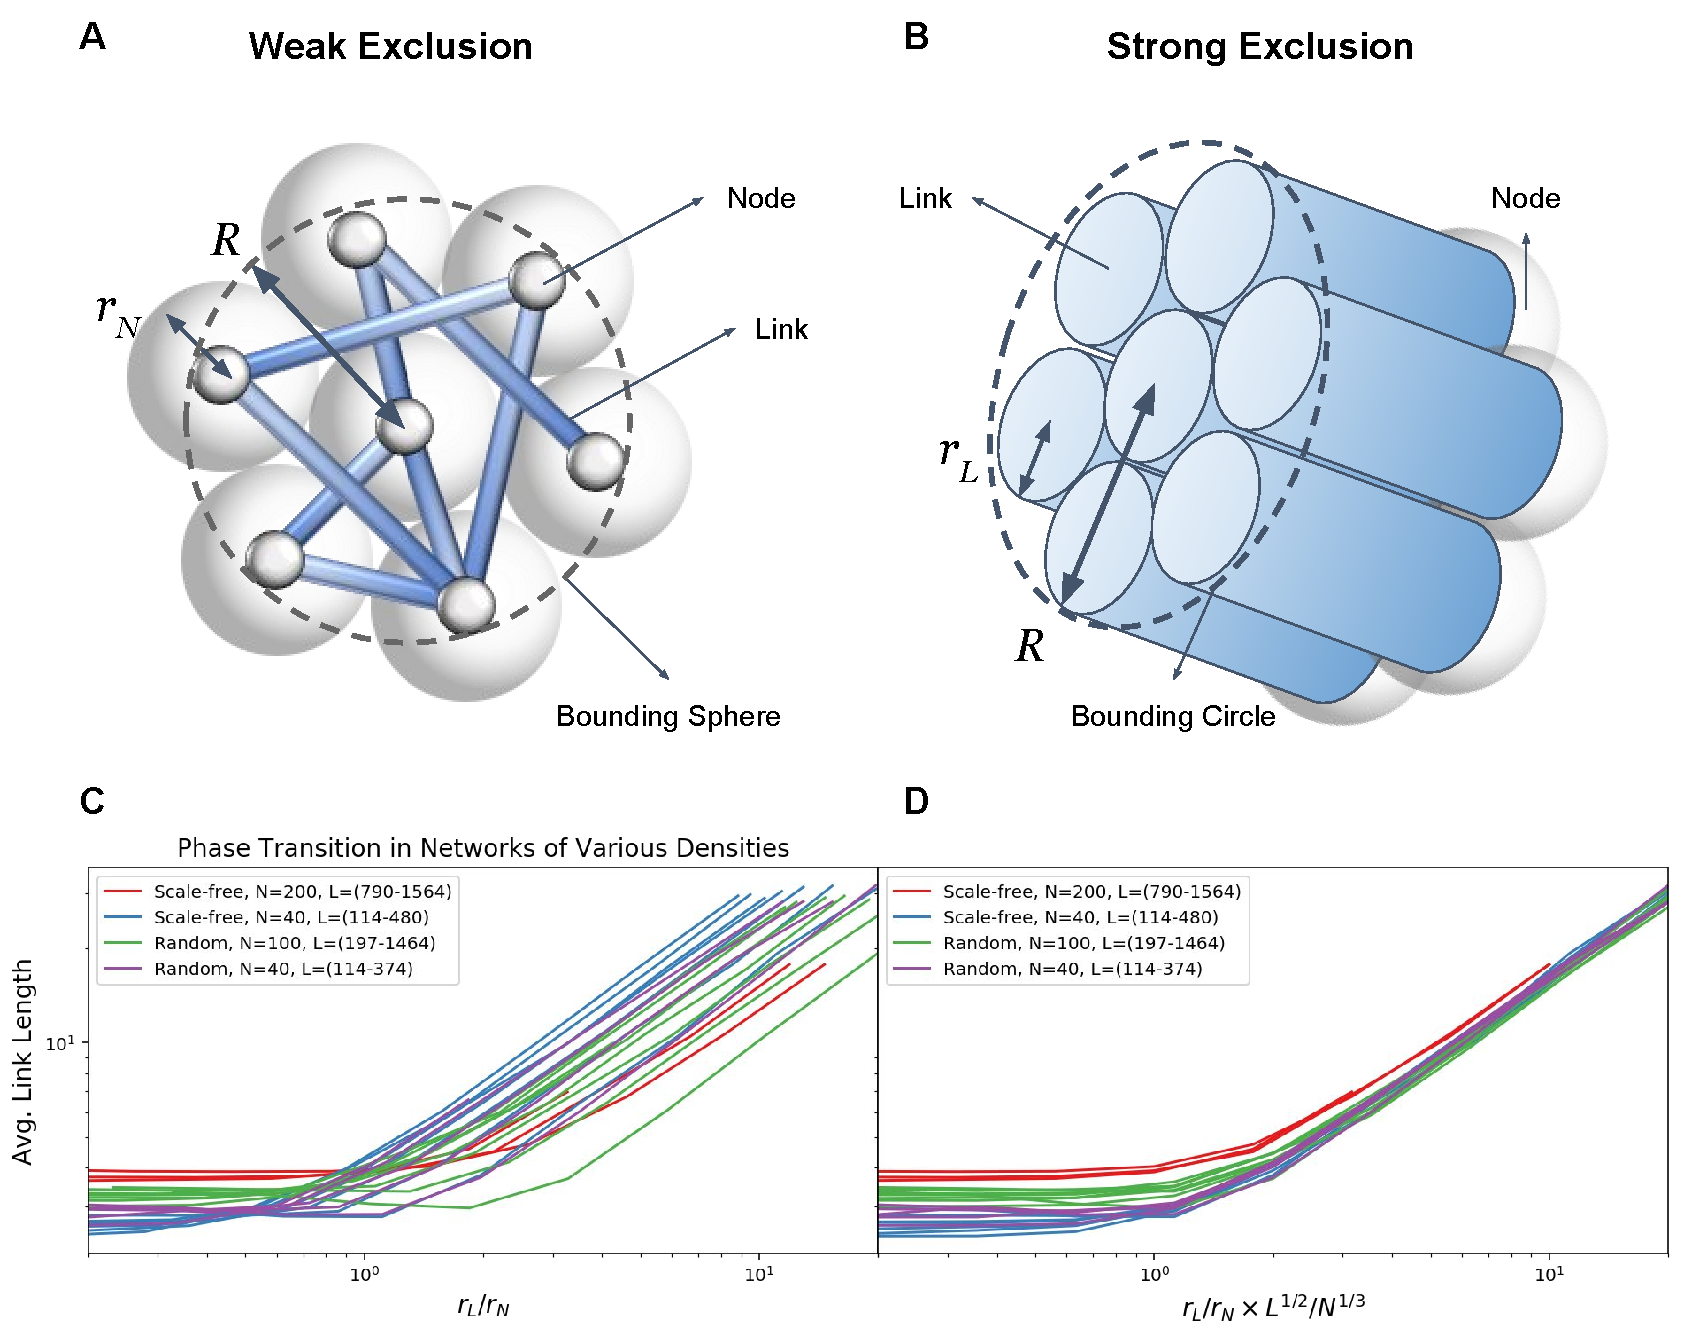
\includegraphics[width=\columnwidth]{fig-09-19/transition-3.pdf}
    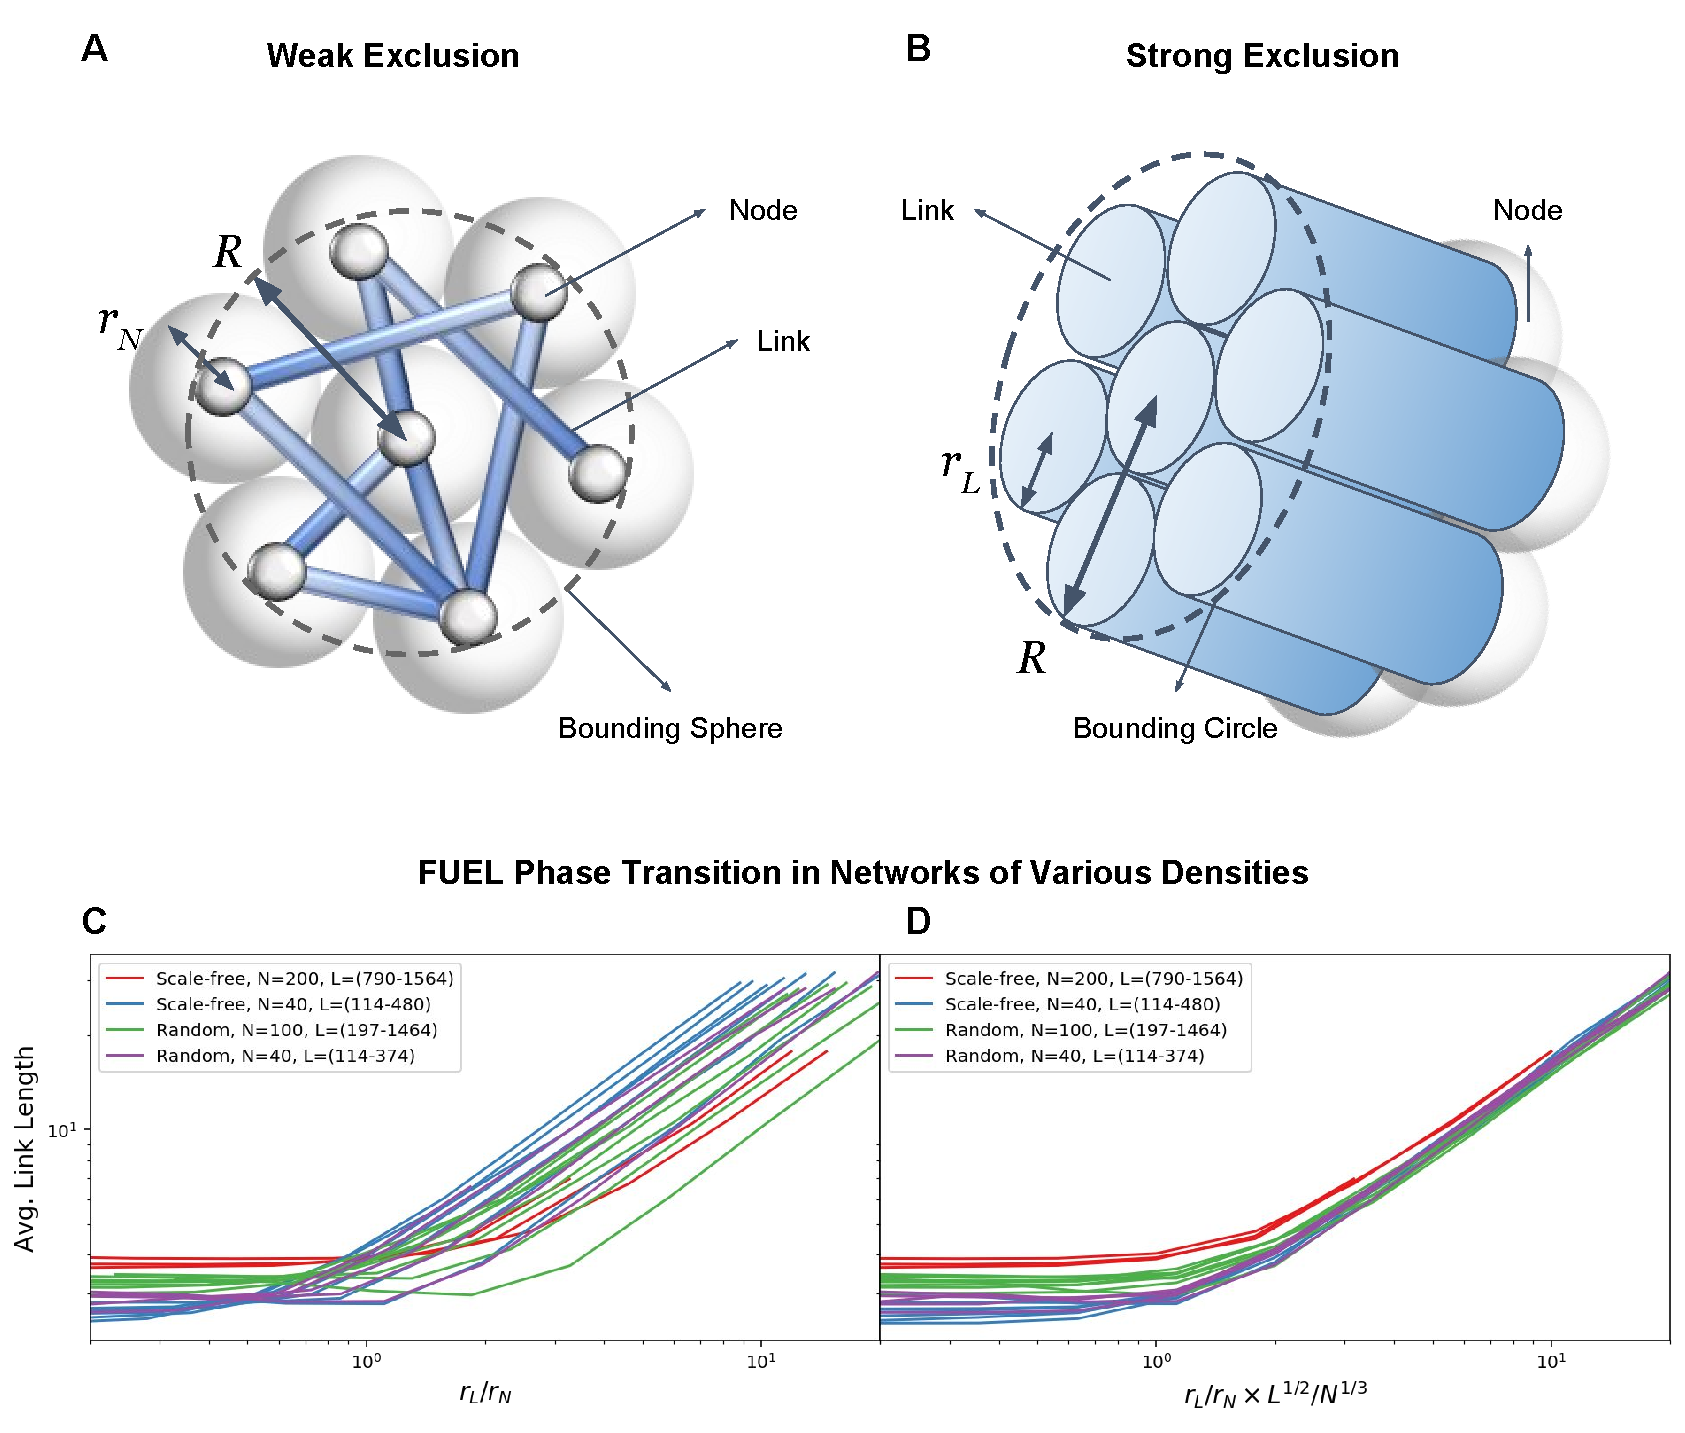
\includegraphics[width=\columnwidth]{fig-09-19/3D-transition.pdf}
    \caption{\scriptsize {\bf (A)} When the links are thin, i.e. $r_L\ll r_N$, they interact only weakly with each other --the weak exclusion regime. 
    In this regime, the range of the node repulsion $r_N$ forces the nodes to stay within $2r_N$ of their neighbors, and links only act as bonds keeping the network together.
    Therefore, the layout size can be estimated by finding radius $R$ of the smallest sphere -- the bounding sphere -- that would encompass $N$ balls of radius $r_N$. 
    {\bf (B)} When links become thick they exclude each other strongly --the strong exclusion regime. 
    Almost all links will feel the push of other links along most of their length. 
    In an ideal scenario, which would occupy the least total volume, links would be locally bundled in parallel with each other (SI sec.\ref{ap:cross}). 
    In this case, the radius $R$ of the bounding circle of the bundle would determine the layout size.
    The area of this bounding circle is approximately the total cross-section of $L$ links. 
    At a thickness where the two estimates for $R$ become comparable, we expect to see a phase transition from the weak to the strong exclusion regime. 
    {\bf C} A plot of average link length versus $r_L/r_N$ for three set of networks with different number of nodes $N$ and links $L$ near the phase transition. The phase transitions are happening at different values of $r_L/r_N$. 
    {\bf D} Rescaling the ratio of $r_L/r_N$ by our analytical prediction for the the transition points makes the curves collapse on similar curves with phase transition happening around near $1$, confirming the estimated transition point. }
    \label{fig:trans}
\end{figure}
The value of $r_L$ when the two estimates for $R$ are comparable provides the critical relative radius 
\begin{equation}
    \tilde{r}_c \equiv {r^c_L\over r_N} \sim N^{1/3} L^{-1/2}. \label{eq:trans}
\end{equation}


We find that the prediction \eqref{eq:trans} offers a reasonable estimate of the numerically obtained transition point for both models (Fig. \ref{fig:trans}C). Indeed, while networks of different number of nodes, $N$, and links, $L$, transition at different points, scaling the $r_L/r_N$ ratio by our theoretical estimate \eqref{eq:trans} places the phase transition near 1 on the x axis (Fig. \ref{fig:trans}D).     
Interestingly, for fixed $N$ and $L$, network of rather different (scale-free, random) topologies show comparable link lengths and similar dependence on $r_L$ (Fig. \ref{fig:phase-compare}D), 
suggesting that the phase diagram of Fig. \ref{fig:phase-compare} are independent of network topology and degree distribution. Most importantly the accuracy of \eqref{eq:trans} tells us that the dramatic transition in the layout and scaling documented in Fig. \ref{fig:phase-compare}A,B,D has its roots in an excluded volume interaction: in the strongly interacting phase such excluded volume interactions dominate the layout; while those interactions are negligible in the weakly interacting regime.

To further characterize the dramatic change in the link structure at $r^c_L$,
we measured the average curvature of each link, normalized by the average link length $\be{l}$.  
We find that the curvature is negligible in the weak exclusion phase, confirming the observation that in this phase the links remain largely straight and conflicts can be avoided by local bendings. 
Beyond $r^c_L$ the curvature rapidly grows, reflecting the need for multiple and often significant bendings to avoid crossings. 
Interestingly, the normalized curvature converges to a constant for large $r_L/r_N$ (Fig. \ref{fig:phase-compare}E), suggesting that in terms of the large scale order parameters average link length and curvature the layouts in the strong exclusion regime at different $r_L/r_N$ have similar characteristics once scaled by layout size.


Finally, we explore how the obtained network's physical properties are changed by explaining its response to external forces. 
This is captured by the Cauchy stress tensor $T_{\mu\nu} \equiv \ro_\mu\ro_\nu V$ \cite{irgens2008continuum}, where $V$ is the total potential energy \eqref{eq:Vfull} (SI sec.\ref{ap:stress}).
Normally, $T_{\mu\nu}$ is determined jointly by the physical properties of the nodes and the links, and the material structure, which in our case is determined by the network topology and its layout. 
We will focus on FUEL, where both nodes and links move freely in response to stress. 

In the weak exclusion regime the links are mostly straight, hence the total stress is dominated by the node terms $V_{NN}$ and $V_{NL}$ in \eqref{eq:Vfull}. 
%It can be shown (SI sec.\ref{ap:stress}) that 
When nodes are scattered uniformly with a fixed coordination number, the components of stress emerging from $V_{NN}$ in \eqref{eq:Vfull} become diagonal (SI sec.\ref{ap:stress}). 
%With the symmetric close-packing, the stress over all nodes yields $\sum_{<ij>} X_{ij\mu}X_{ij\nu} = \delta_{\mu\nu}$, where $<ij>$ indicates nodes within a distance $2r_N$ of each other. 
However, in a network environment nodes are surrounded by a varying number of other nodes, leading to shear (off-diagonal) stress components, common in solids and high viscosity fluids. This implies that the stress does not spread uniformly in all directions, indicating that networks in the weak exclusion phase have solid-like properties. 
In the strong exclusion phase, where the links fill up the space and push on each other,
the link contributions $V_{el}+V_{LL}$ in \eqref{eq:Vfull} dominates $T_{\mu\nu}$. 
The adjacent link segments will be at a distance $|x_l-x_m| = \be{r} = 2 r_L$, hence the space-filling and uniformity will result in a diagonal total stress tensor (SI sec.\ref{ap:stress}) %(integrated over the whole network) 
\begin{equation}
    \mbox{}\int d^3x  T_{\mu\nu} \approx \left[ k + {L \be{l}^2\over 4r_L^2}   \right]\delta_{\mu\nu} \label{eq:Tstrong}
,\end{equation}
%
describing a hydrodynamic stress with pressure $ p =  k + {L \be{l}^2/( 4r_L^2)}$. Therefore, we predict in the strong exclusion limit networks displays a fluid-like response to external stress. 
But, unlike molecules in a liquid or a gas, link segments are not free to diffuse or move freely. Consequently a more accurate description is that of a gel, a reminiscent of a pool of cross-linked polymers, which is soft and whose components are stationary, unless external forces act on them. 
%Since parts of links are not free to move far apart from each other (i.e. the mean free path of particles is much smaller than the system size) this fluid does not behave like a gas, but rather like a liquid or soft gel. The key difference between a gel and a liquid is that in liquids particles may diffuse and thus correlation in positions is lost, while 
In a gel, cross-linked polymers provide a scaffold and relative structural integrity, similar to the configuration observed in the strong exclusion phase. 
% Thus, we conclude that layouts in the strong exclusion phase are better characterized as gels.  

To test the validity of the predicted solid-gel transition, %we measure the diagonal terms of $T_{\mu\nu}$, checking if they satisfy the hydrodynamic conditions $T_{\mu\mu}=p$ for all $\mu=x,y,z$, which is expected in the fluid-gel phase but not in the solid phase. 
% To be specific, 
we measured the tensile forces, 
$ \sigma_\mu \equiv T_{\mu\mu}$, by placing the networks generated by FUEL between two walls compressing them in the $y$ direction by $10\%$ of its equilibrium height and evaluate the change in forces throughout the network (Fig. \ref{fig:stress}A, SI sec.\ref{ap:stress}). 
We break the tensile stress into two components: $\sigma_\parallel$ and $\sigma_\perp$, parallel and perpendicular to the direction of compression.  
If the stress components $\sigma_x, \sigma_y$ and $\sigma_z$ have similar magnitude, as in hydrostatics, we have $ \sigma_\parallel ={1\over L^3} \int_\mathrm{net} d^3x |\sigma_y| = p$ and $\sigma_\perp = {1\over L^3} \int_\mathrm{net} d^3x \sqrt{\sigma_x^2+ \sigma_z^2} = \sqrt{2} p$, consequently
% \begin{align}
% \be{\sigma_\parallel} &={1\over L^3} \int_\mathrm{net} d^3x |\sigma_y| = p\cr
% \be{\sigma_\perp} &= {1\over L^3} \int_\mathrm{net} d^3x \sqrt{\sigma_x^2+ \sigma_z^2} = \sqrt{2} p \label{eq:sigp}   
% \end{align}
 $ \sigma_\parallel/\sigma_\perp = 1/\sqrt{2}$.
%The integral is over the volume of the layout and $L^3$ represents total layout volume.
If, on the other hand, the ratio $ \sigma_\parallel/\sigma_\perp$ is orientation-dependent, varying as we rotate the layout, the network %has different elastic moduli in different directions, and so it 
possesses solid-like properties. 
\begin{figure}
    \centering
    %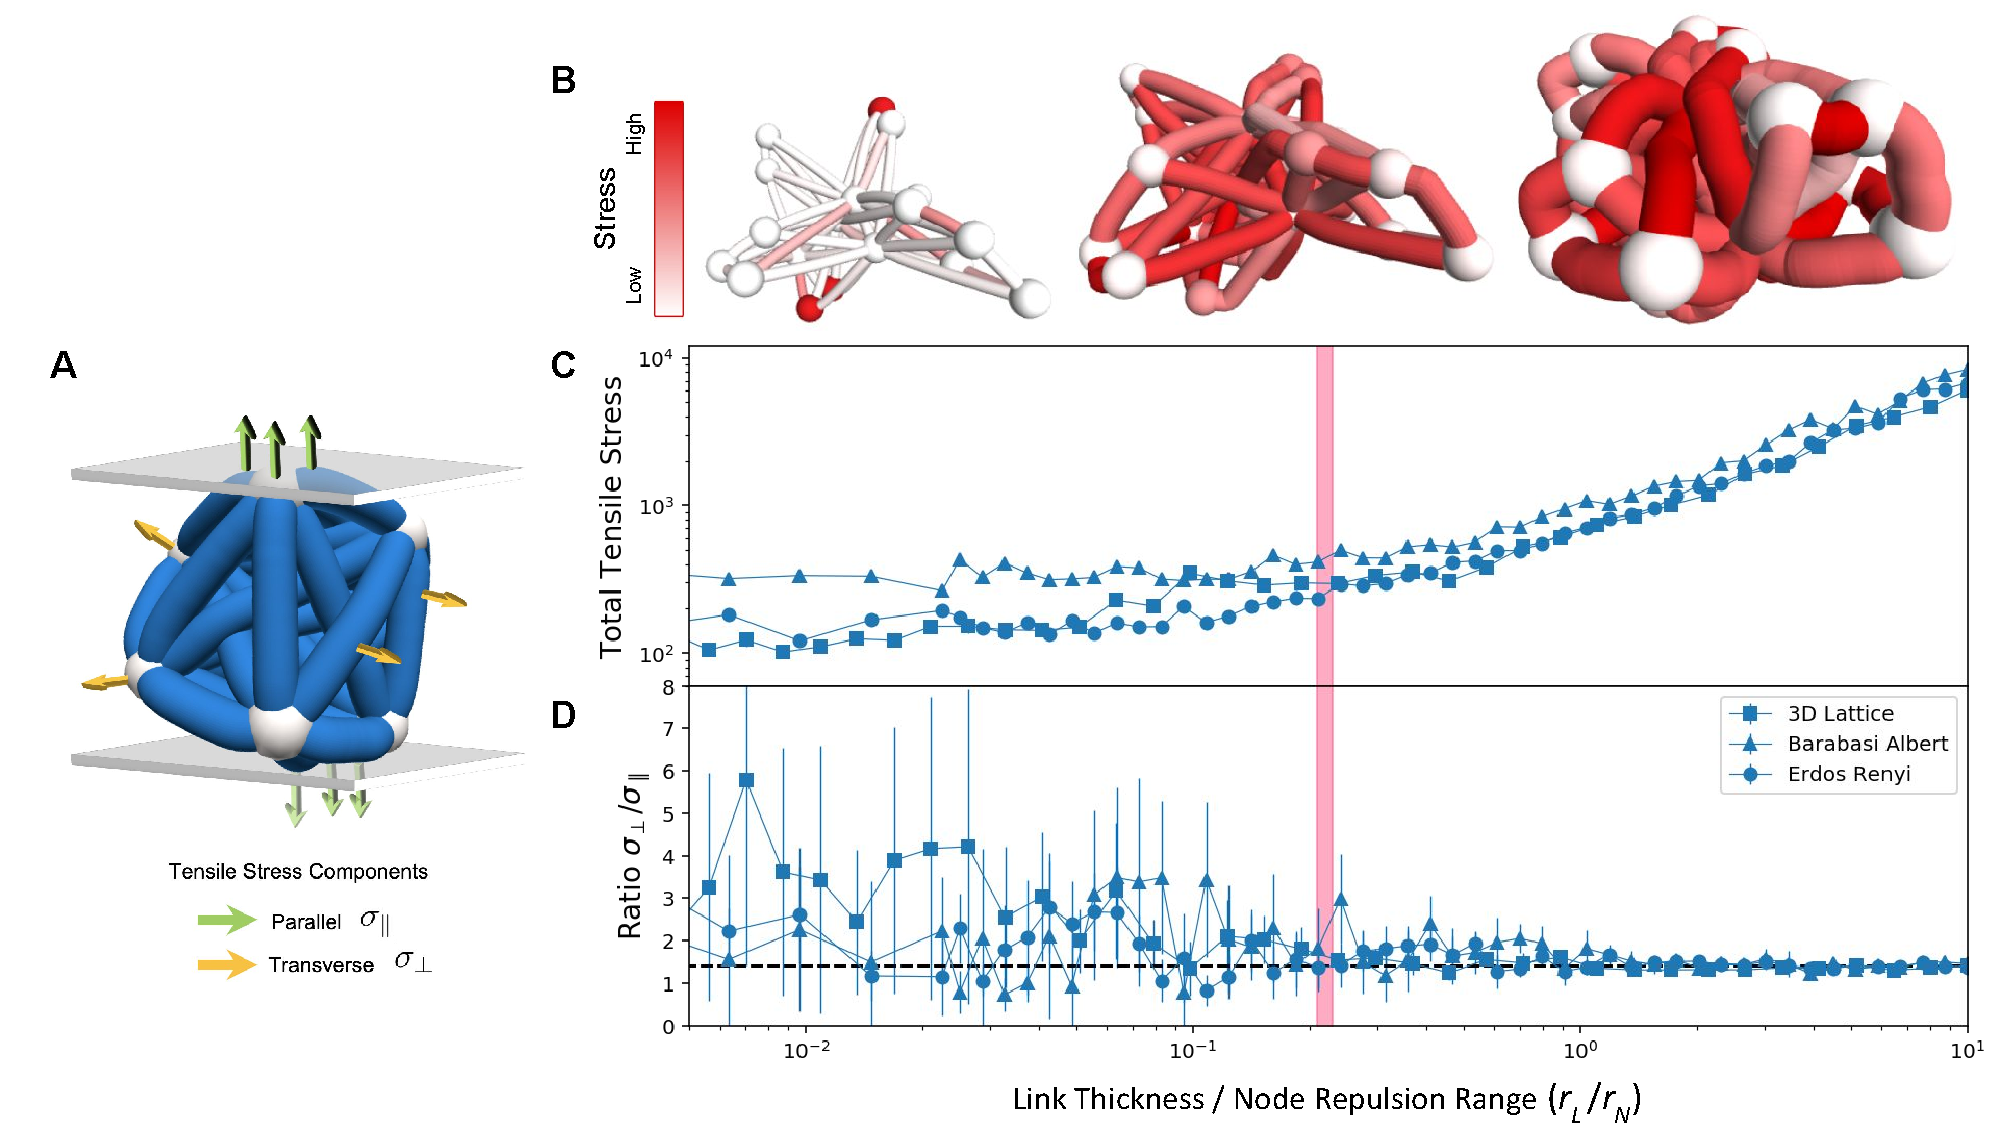
\includegraphics[width=1\columnwidth]{fig-09-19/stress-plots-3.pdf}
    % 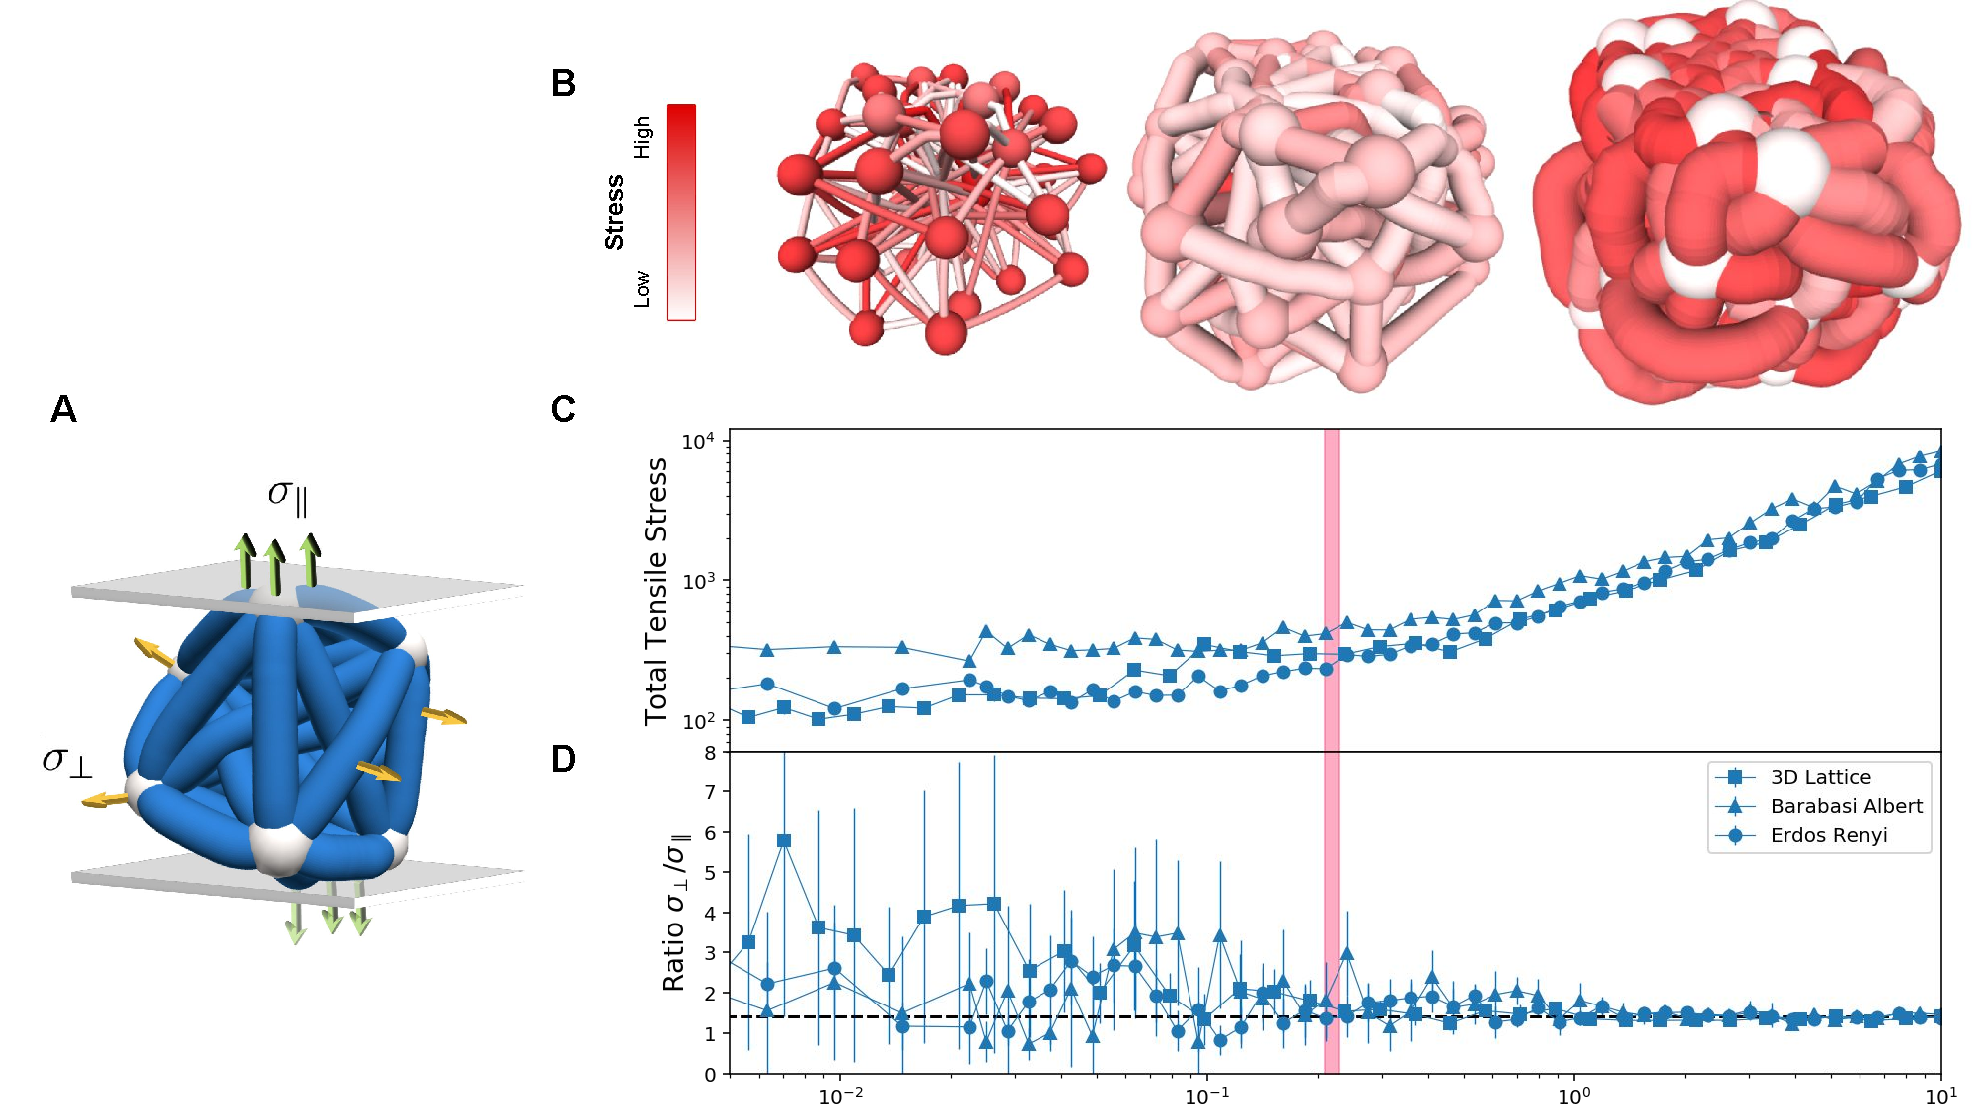
\includegraphics[width=1\columnwidth]{fig-09-19/stress-2.pdf}
    % 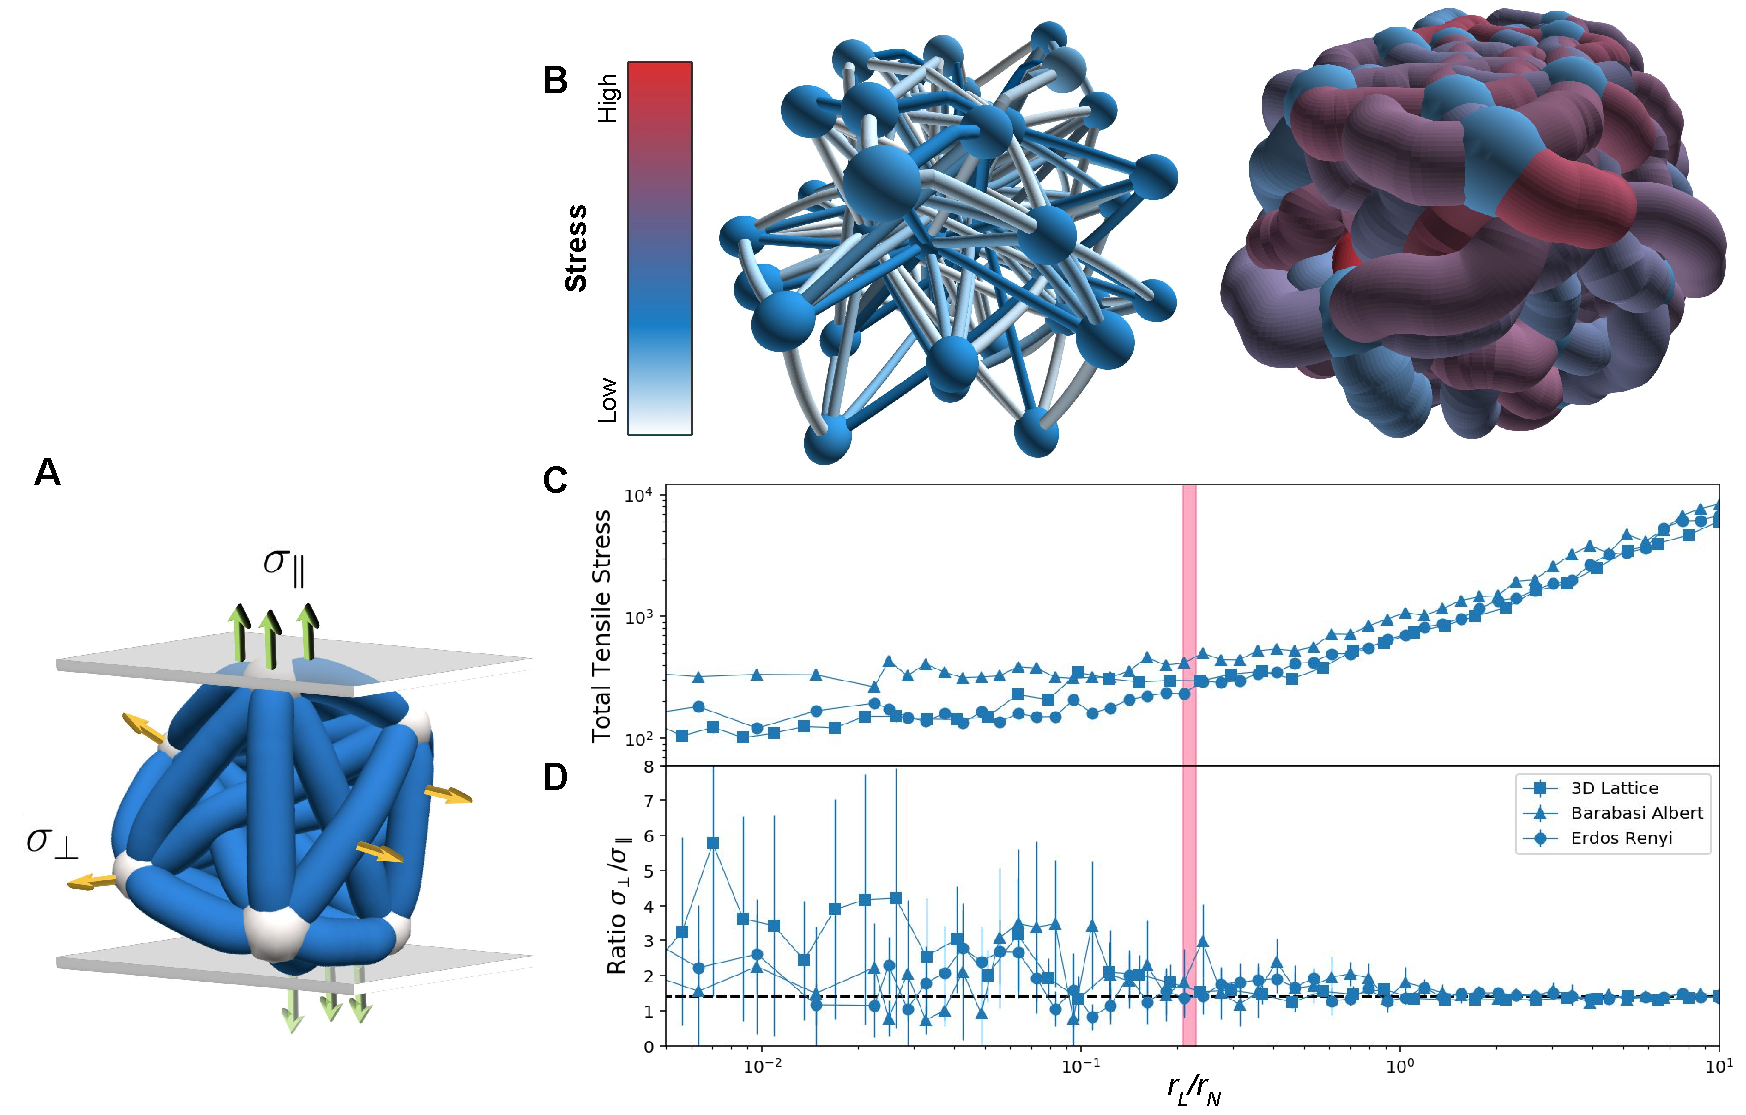
\includegraphics[width=1\columnwidth]{fig-09-19/stress-4.pdf}
    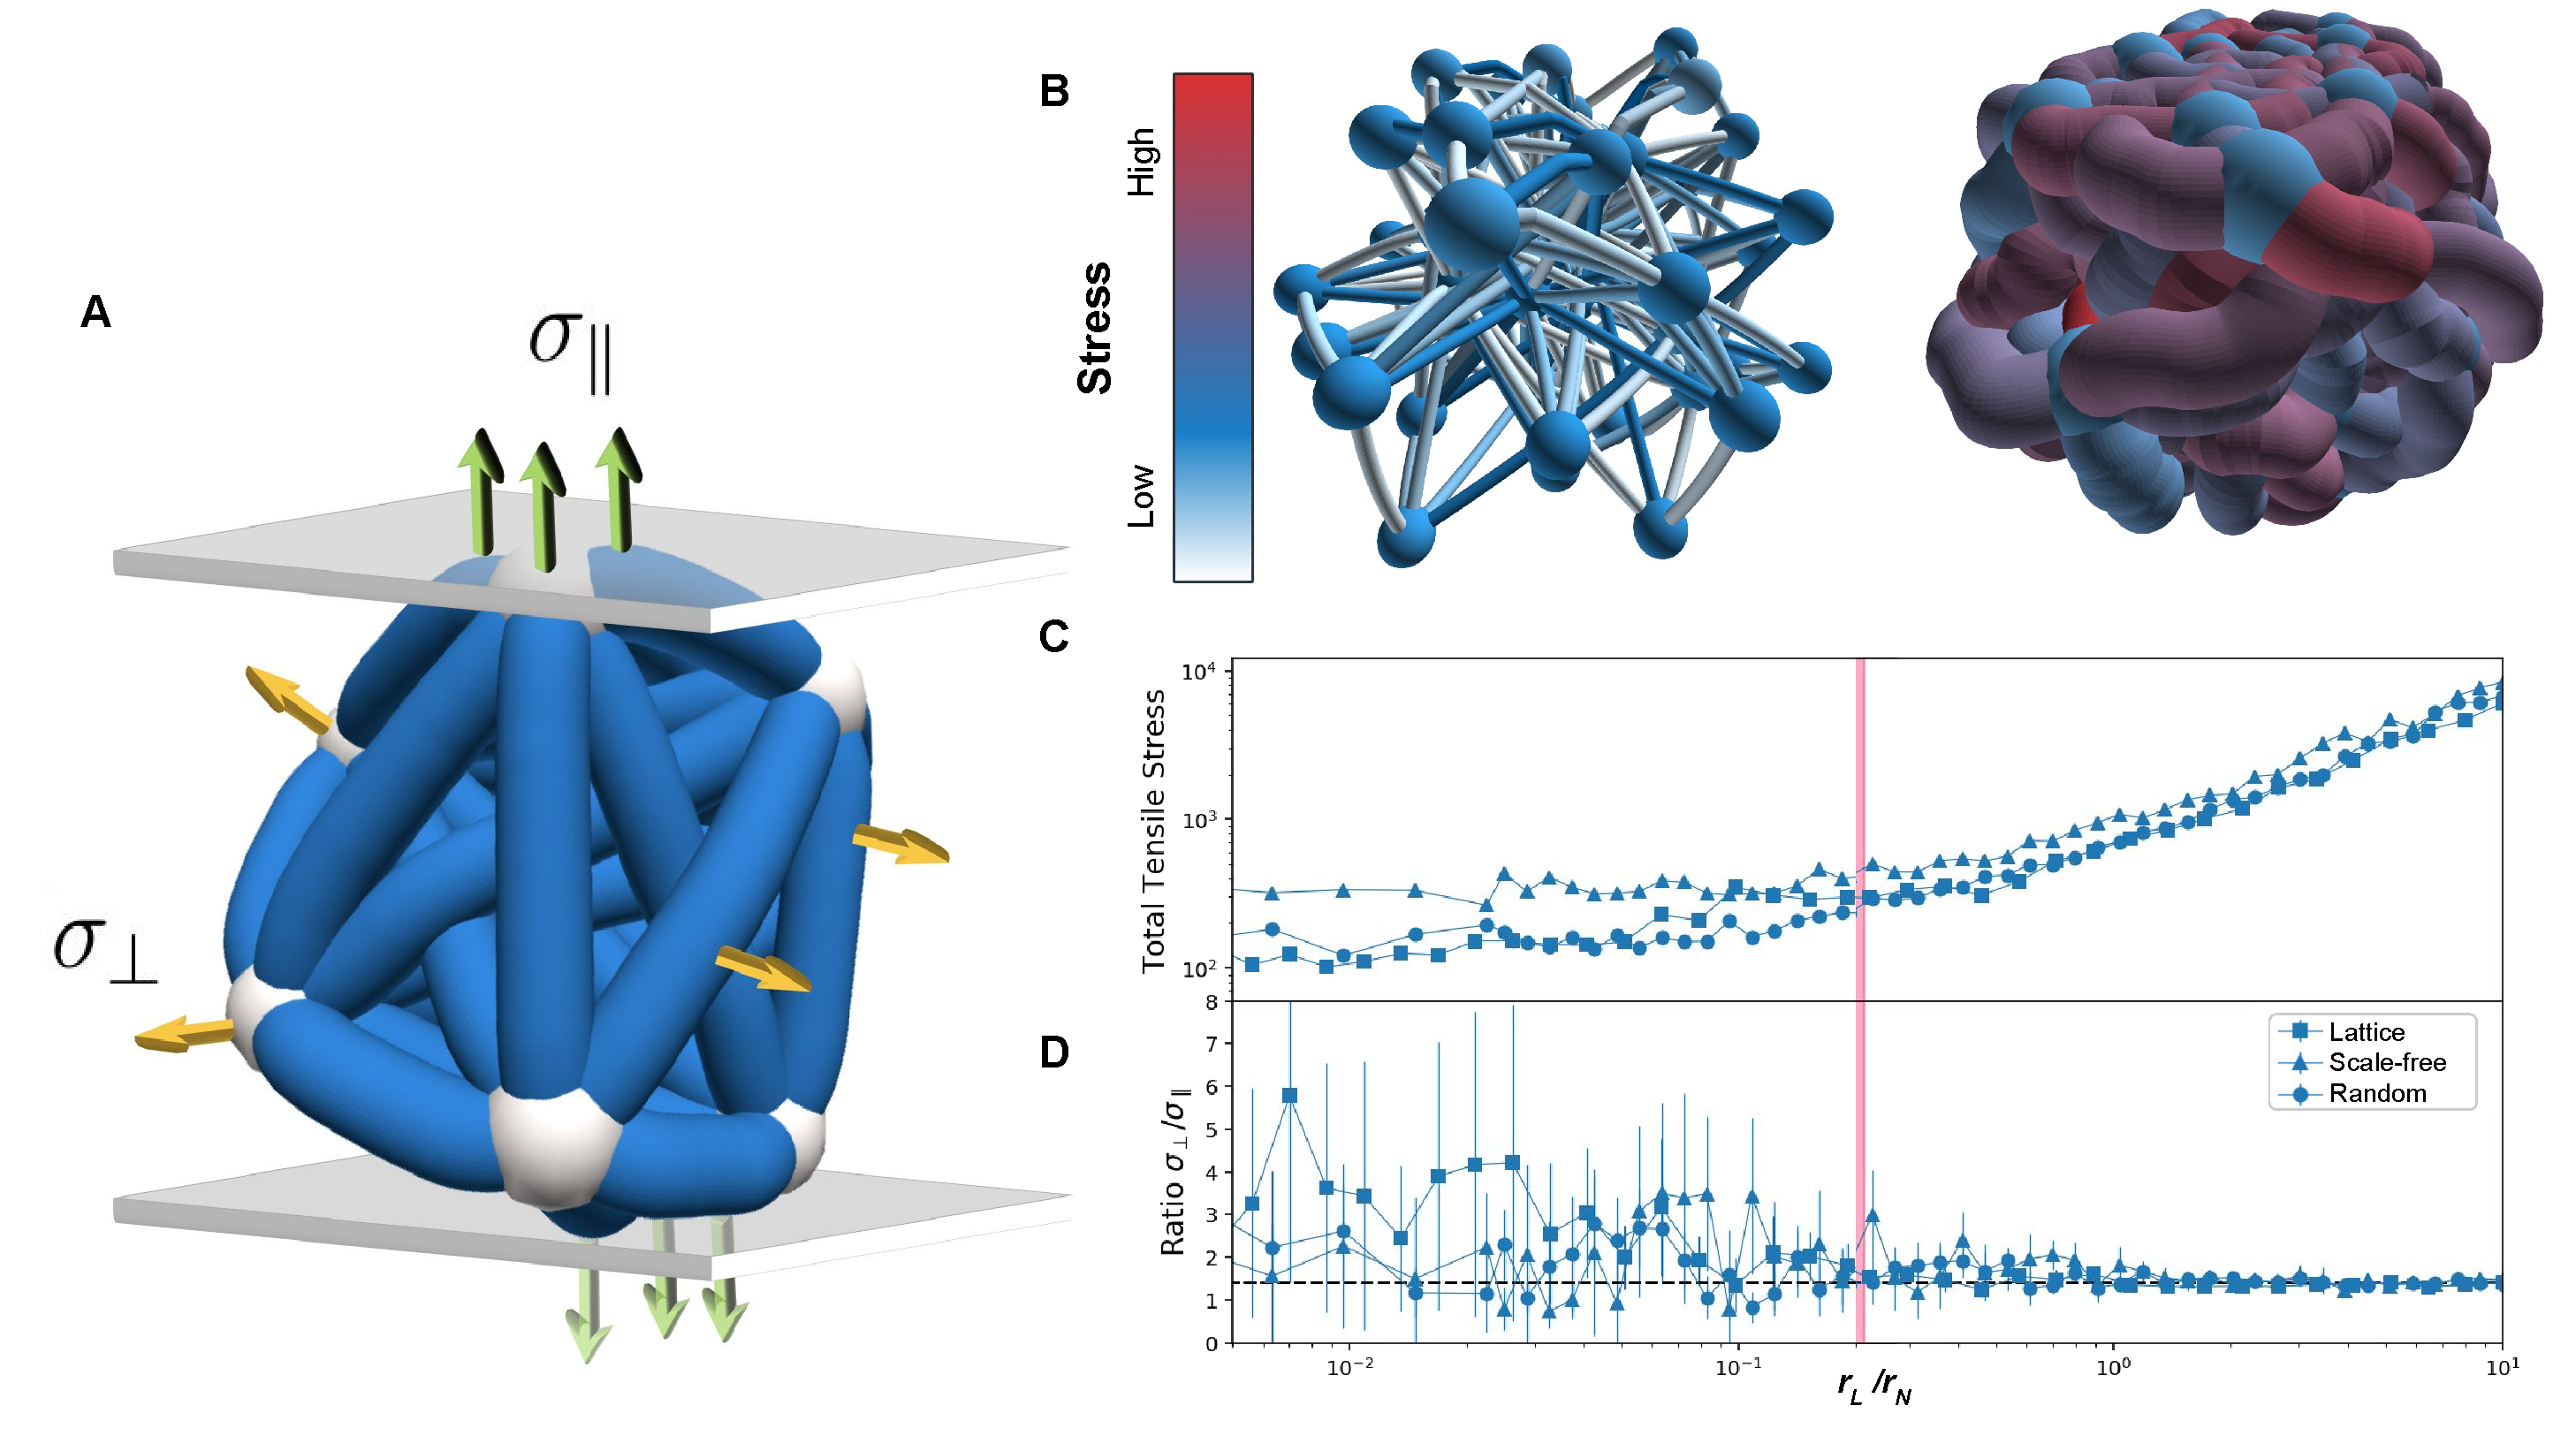
\includegraphics[width=1\columnwidth]{fig-09-19/stress-071917.pdf}
    \caption{\scriptsize
    {\bf (A)} A sketch of tensile stress build-up in a network as a result of confinement between two walls in the vertical direction. 
    The walls have compressed the network in the vertical direction by a small amount.
    The green arrows show forces pushing vertically on the walls, i.e. the component of local tensile stress parallel to the direction of compression. 
    We denote this by $\sigma_\parallel(x)$. 
    Yellow arrows indicate the tensile stress in directions $\sigma_\perp(x)$
    perpendicular to the compression. 
    {\bf (B)} Examples of layouts showing total stress (more red means more stress).  
    Each network corresponds to the  link thicknesses in the plots below them.
    Notice that in the weak exclusion (left) most of the stress is concentrated in a few nodes and most links show very little stress. 
    %Near the phase transition (middle) both nodes and links show a stress, and 
    In the strong exclusion phase (right) almost all of the stress is in the links. 
    {\bf (C)} Total Stress of different topologies as a function of link thickness. Since the definition of $x,y,z$ is frame-dependent, we measure the forces for 50 random network orientations. 
    %Because networks are inhomogeneous objects, stress is averaged over 50 random network orientations. 
    The weak exclusion phase shows a very slowly increasing level of stress for increasing thicknesses. %, but the value also fluctuates a lot at different orientations (SI sec.\ref{ap:stress}). 
    Around the transition point, the trend changes and in the strong exclusion phase stress grows almost linearly with link thickness. 
    In this phase stress in links becomes larger than stress in nodes (SI sec.\ref{ap:stress}). 
    {\bf (D)} The ratio of parallel and transverse tensile stress $\sigma_\perp/\sigma_\parallel$, with errorbars showing its fluctuation over the 50 random orientations of the layout. 
    In the weak exclusion phase, the ratio depends on layout orientation. This generally happens in amorphous solids, where local molecular structure spreads stress in a random manner dependent on the direction of compression. 
    As we transition into the strong exclusion phase, the fluctuations of $\sigma_\perp/\sigma_\parallel$ gradually decay to zero, and $\sigma_\perp/\sigma_\parallel \approx \sqrt{2}$. 
    This is the value expected in a non-viscous fluid where all three components of tensile stress become equal to the pressure.}
    \label{fig:stress}
\end{figure}
\outNim{
\begin{figure}
    \centering
    %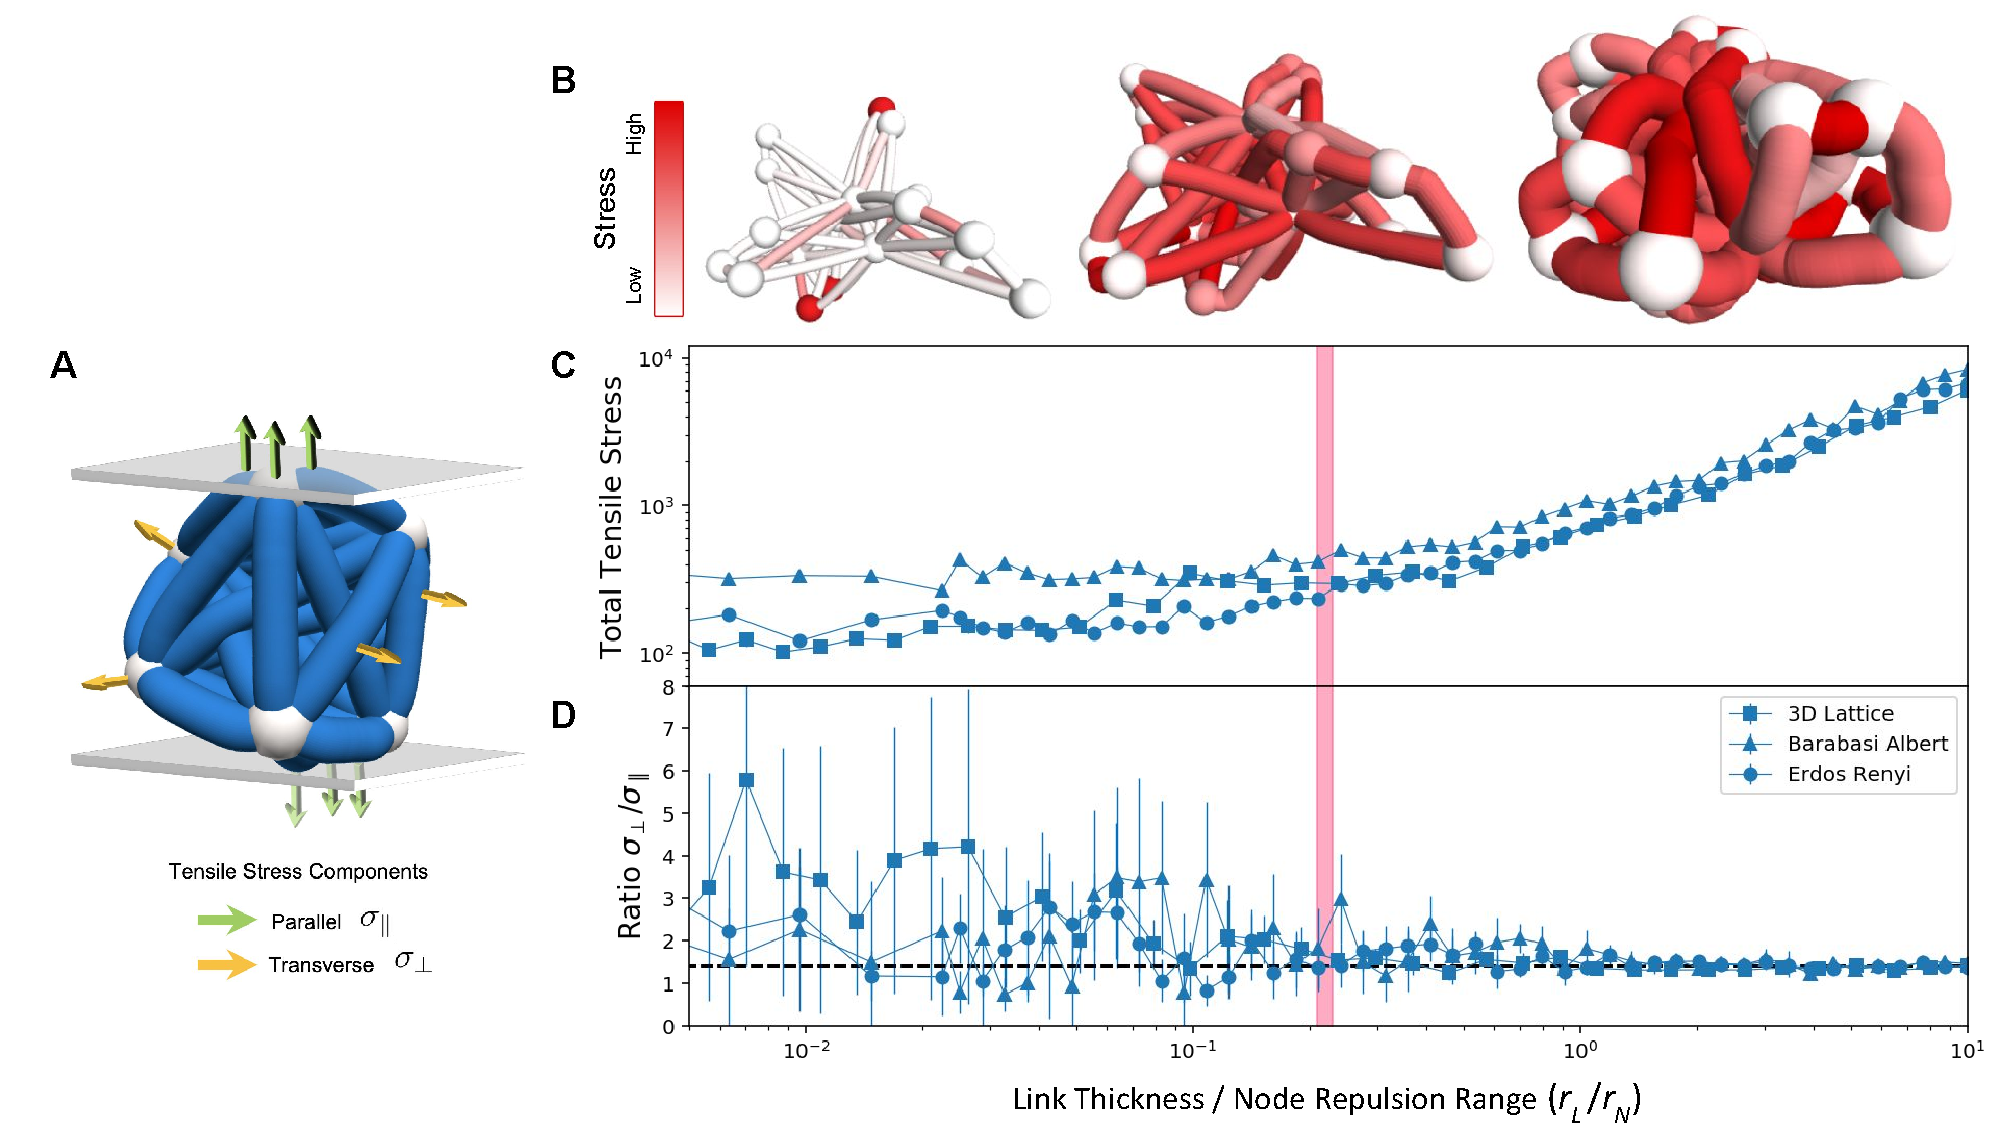
\includegraphics[width=1\columnwidth]{fig-09-19/stress-plots-3.pdf}
    % 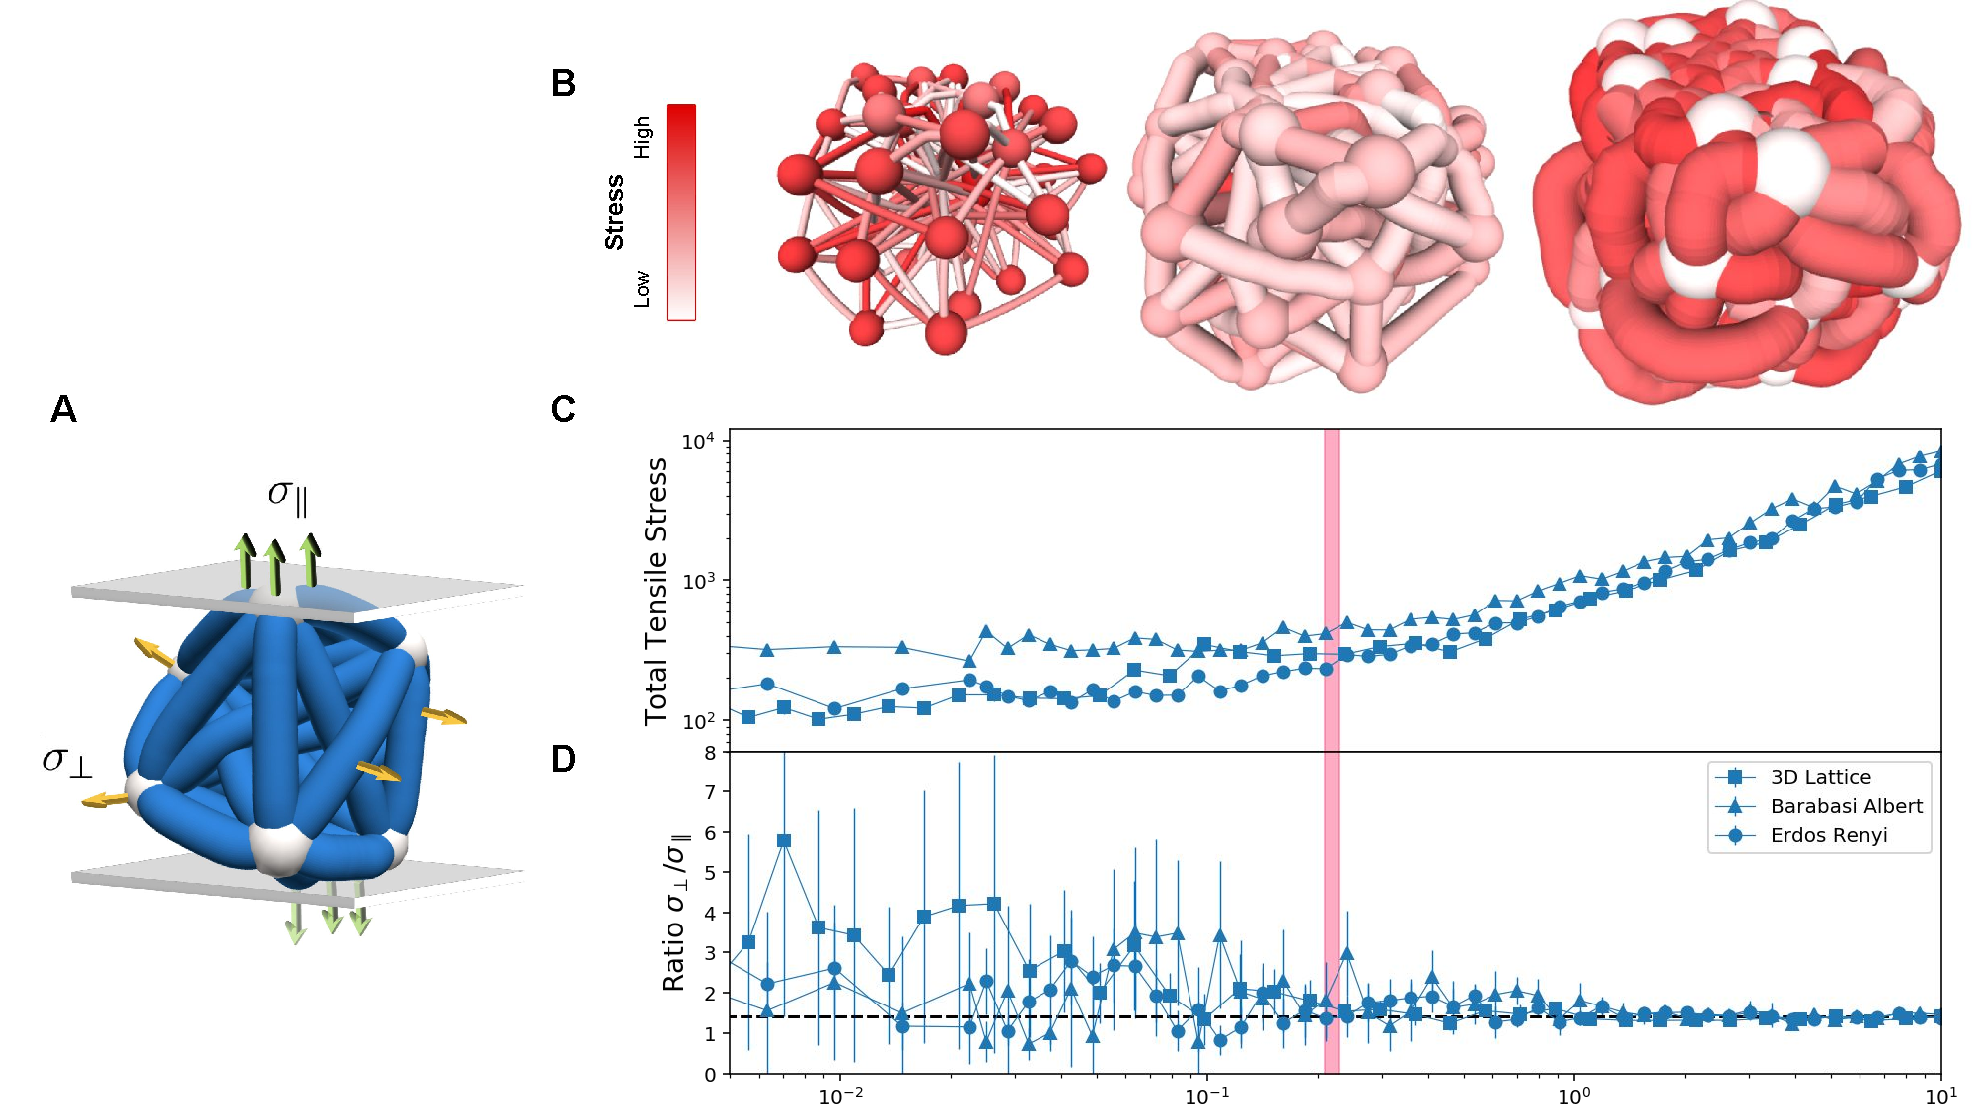
\includegraphics[width=1\columnwidth]{fig-09-19/stress-2.pdf}
    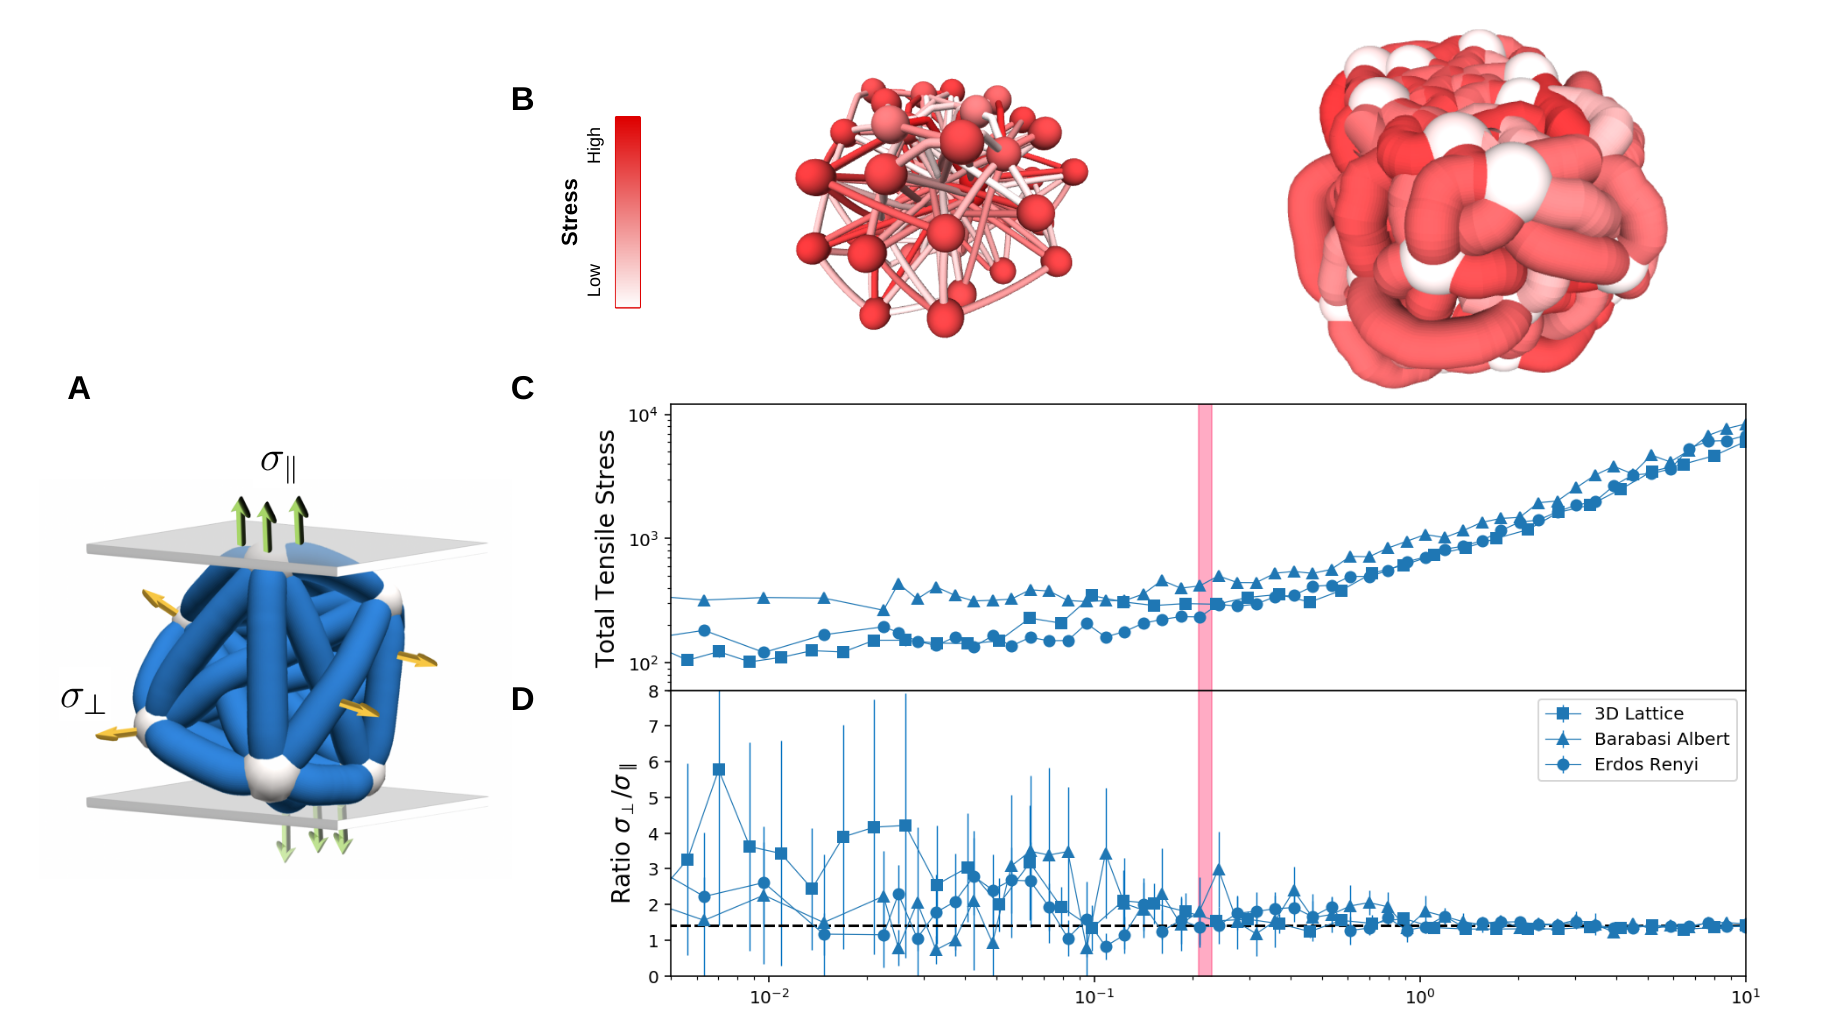
\includegraphics[width=1\columnwidth]{fig-09-19/stress-3.png}
    \caption{\scriptsize
    {\bf (A)} A sketch of tensile stress build-up in a network as a result of confinement between two walls in the vertical direction. 
    The walls have compressed the network in the vertical direction by a small amount.
    The green arrows show forces pushing vertically on the walls, i.e. the component of local tensile stress parallel to the direction of compression. 
    We denote this by $\sigma_\parallel(x)$. 
    Yellow arrows indicate the tensile stress in directions $\sigma_\perp(x)$
    perpendicular to the compression. 
    {\bf (B)} Examples of layouts showing total stress (more red means more stress).  
    Each network corresponds to the  link thicknesses in the plots below them.
    Notice that in the weak exclusion (left) most of the stress is concentrated in a few nodes and most links show very little stress. 
    %Near the phase transition (middle) both nodes and links show a stress, and 
    In the strong exclusion phase (right) almost all of the stress is in the links. 
    {\bf (C)} Total Stress of different topologies as a function of link thickness. Because networks are inhomogeneous objects, stress is averaged over 50 random network orientations. The weak exclusion phase shows a very slowly increasing level of stress for increasing thicknesses. %, but the value also fluctuates a lot at different orientations (SI sec.\ref{ap:stress}). 
    Around the transition point, the trend changes and in the strong exclusion phase stress grows almost linearly with link thickness. 
    In this phase stress in links becomes larger than stress in nodes (SI sec.\ref{ap:stress}). 
    {\bf (D)} The ratio of parallel and transverse tensile stress $\sigma_\perp/\sigma_\parallel$, with errorbars showing its fluctuation over the 50 random orientations of the layout. 
    In the weak exclusion phase, the ratio depends on layout orientation. This generally happens in amorphous solids, where local molecular structure spreads stress in a random manner dependent on the direction of compression. 
    As we transition into the strong exclusion phase, the fluctuations of $\sigma_\perp/\sigma_\parallel$ gradually decay to zero, and $\sigma_\perp/\sigma_\parallel \approx \sqrt{2}$. 
    This is the value expected in a non-viscous fluid where all three components of tensile stress become equal to the pressure.}
    \label{fig:stress}
\end{figure}
} %%% out
%
\outNim{
\begin{figure}
    \centering
    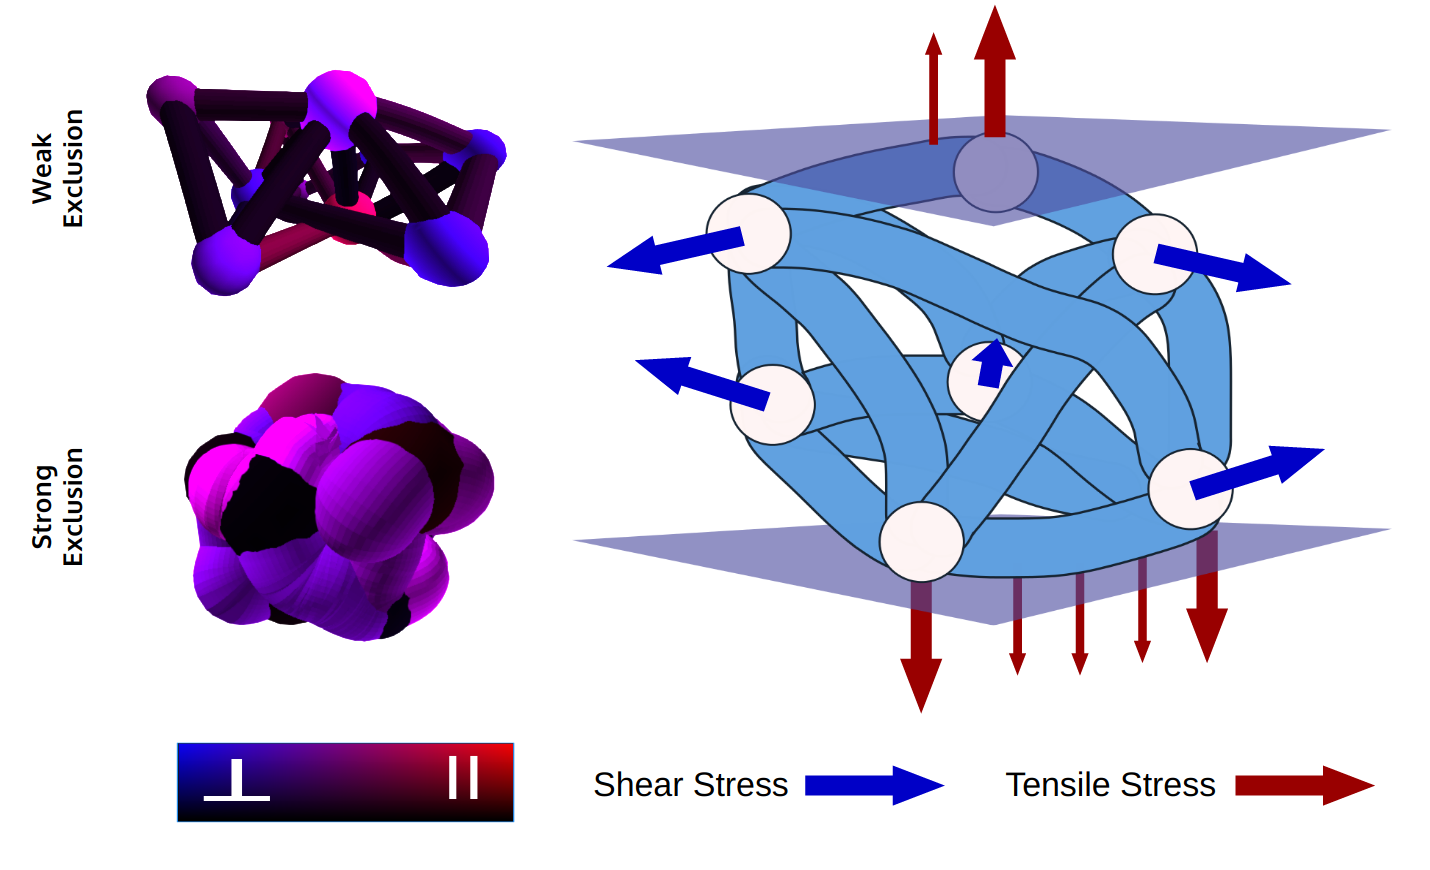
\includegraphics[width = .7\columnwidth]{fig-09-19/stress-ex.png}
    \caption{Right: A sketch of tensile stress build-up in a network as a result of confinement between two walls in the vertical direction. 
    The walls have compressed the network in the vertical direction by a small amount. %$\delta \vec{x}$. 
    The red arrows show the node (thick) and link (thin) forces pushing vertically on the walls.  
    These make up the component of local tensile stress which is parallel to the direction of compression. 
    We denote this by $\sigma_\parallel(x)$. 
    Blue arrows indicate the tensile stress in directions 
    %local shear stress $\tau(x)$ in nodes, i.e. stress 
    transverse to the direction of compression (for clarity, link transverse stress is not shown).
    Left: Examples of tensile ($\parallel$, red) and transverse ($\perp$, blue) stress in networks in the strong exclusion (top) and weak exclusion (bottom) phases. 
    The mixture of blue and red indicates the relative magnitude of the parallel and transverse tensile stress respectively. Darker means smaller total stress. 
    In the strong exclusion phase, all links show stress, whereas in the weak exclusion phase only a few have significant stress. 
    The strong exclusion phase shows more parallel tensile stress at the walls and more transverse stress in the mid parts. 
    The weak exclusion phase, on the other had, shows mostly tensile stress in links, mostly due to change in their length via the compression.}
    \label{fig:stress}
\end{figure}
}%%%%%
%Stress measures the changes in internal forces\footnote{Although formally, it requires defining surfaces and measuring components of force normal or parallel to the surface, since we only want the total stress that builds up in the network we simply measure the changes in internal forces in the layout as a result of compression.} under external forces.
%These internal forces yield the  diagonal elements $ \sigma_\mu \equiv T_{\mu\mu}$, whose trace provides the pressure $\sum_\mu T_{\mu\mu} = 3p$. 
%Moreover, if the three diagonal  components $T_{xx}, T_{yy}$ and $T_{zz}$ are similar, the network is showing a characteristic of hydrodynamics.
%In other words,
% To measure $\sigma_\mu$ we measure the change in forces throughout the network after compressing the network in one direction by a small amount (SI sec.\ref{ap:stress}). 
% We, compressed the networks in the $y$ direction by $10\%$ of its original equilibrium height. 


We measured the total stress for varying $r_L/r_N$, observing a transition from a roughly constant stress value in the weak exclusion regime to a monotonically increasing total stress in the strong exclusion regime (Fig. \ref{fig:stress}C). 
The transition occurs around $\tilde{r}_c$ predicted by \eqref{eq:trans}, indicating that the change in the system's behavior is indeed caused by the excluded volume induced transition from a node to a link-dominated layout.  
We also examined whether the $ \sigma_\parallel/ \sigma_\perp$ ratio is constant,
% We find that, as predicted by the theory, $\sigma_\parallel/\sigma_\perp$ fluctuates significantly for node stress at almost all (except at very high) link thicknesses, indicating that it does not satisfy the hydrostatic condition (Fig. \ref{fig:stress}D).%(SI sec.\ref{ap:stress}).
% In contrast, the stress in links shows a remarkably constant  $\sigma_\parallel/\sigma_\perp$ ratio starting at thicknesses well below the phase transition, indicated by a red strip (SI). 
% At very low thicknesses link stress too shows large fluctuations. 
% And finally, when we add the node and link stress, 
finding that the total stress displays large fluctuations in the weak exclusion regime, as we rotate our network, indicative of an anisotropic solid-like behavior. 
These fluctuations largely vanish at the transition, where the ratio  reaches the hydrodynamic ratio $\sigma_\parallel/\sigma_\perp = 1/\sqrt{2}$  (Fig. \ref{fig:stress}D), as we would expect if we place a fluid or a gel under pressure. 

\outNim{
\begin{figure}
    \centering
    \vspace{10cm}
    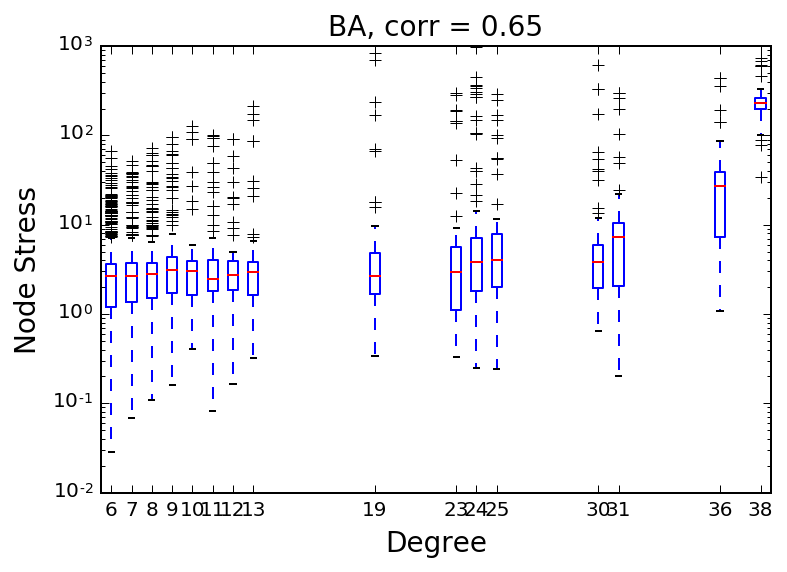
\includegraphics[width=.4\columnwidth]{fig-09-19/stress-deg-ba.png}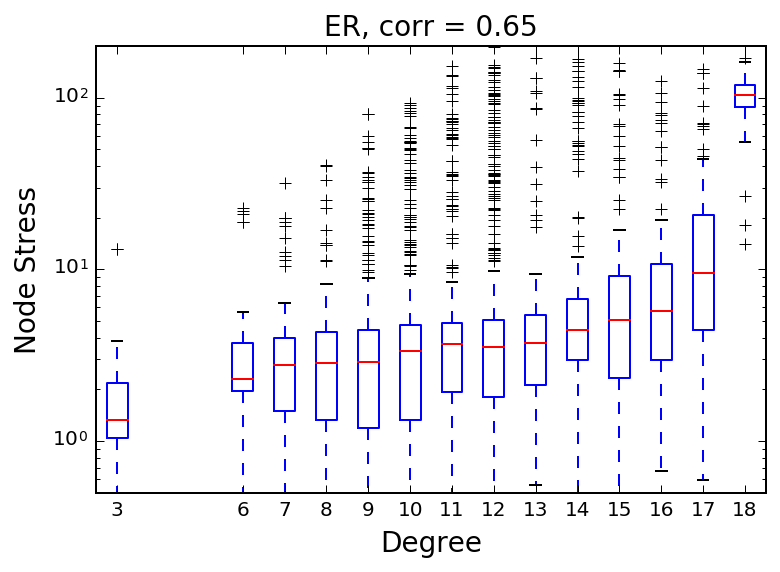
\includegraphics[width=.4\columnwidth]{fig-09-19/stress-deg-er.png}
    
    \caption{Distribution of stress in nodes vs. degree in BA (left) and ER (right), oth with 49 nodes and 280 links. The spread is from layouts at different thicknesses. The Pearson correlation between degree and node stress is 0.61 in BA and 0.58 in ER.}
    \label{fig:stress-k}
\end{figure}

\begin{figure}
    \centering
    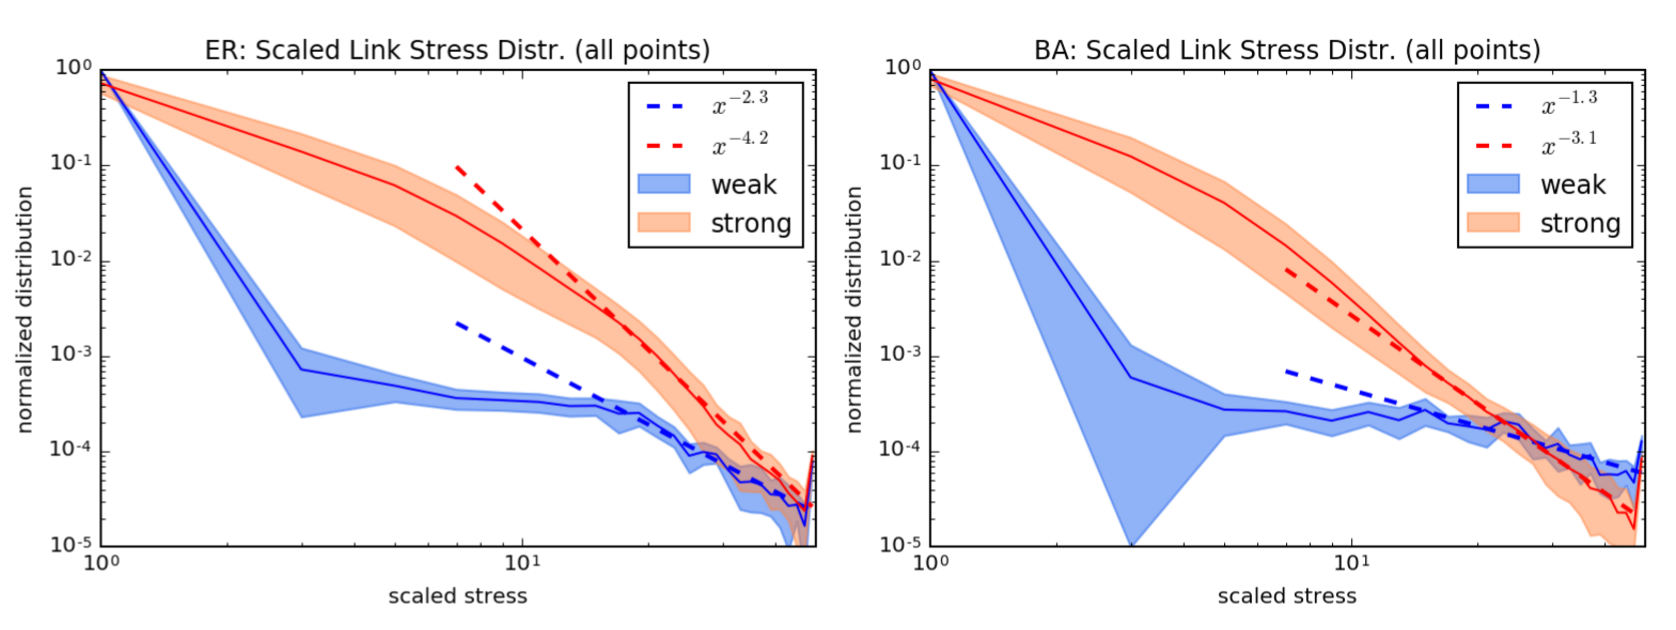
\includegraphics[width=.8\columnwidth]{fig-09-19/stress-dist.png}
    \caption{Distribution of stress along links in the weak (blue) and strong (orange) exclusion phases. Left is in ER and right is in BA. }
    \label{fig:Tdist}
\end{figure}

} %%%


\newpage
%\section*{Discussion}
In summary, the developed modeling framework to lay physical networks out in 3D predicts the existence of two distinct phases: a weak exclusion phase whose layout is similar to the FDL-based layout and crossings may be present, but can be avoided via local link bendings; and a more 
%The most 
interesting strong exclusion phase, whose characteristics are dominated by link crossings.
%{\color{red} ALL topologies in one place} In conclusion, w
We find that the transition between weak and strong exclusion phase is driven by excluded volume interactions and hence it is universal, meaning that networks with different topologies and constraints display the transition at the same critical point, and behave similarly in the two regimes. 
%Indeed, the network parameters, i.e. number of nodes and links, are the only factors that characterize the volumetric properties of these networks. 
%This suggests that, if the only constraint is minimizing the volume, then regardless of how complicated a network topology is, for a fixed density, the phase diagram of average link length should be achieved.
%\footnote{It remains to be checked how network density would affect the outcome and whether going to lower densities would lead to layout properties that differ among different topologies in the strong exclusion phase.}.
We also find that the universal (strong exclusion) phase behaves like a gel under stress, whereas the weak exclusion phase has solid-like properties. 

The consequences of the physical constraints in 3D embedding introduces a new layer of complexity and may potentially affect dynamical and functional properties of networks. Case in point is the brain, a three dimensional physical network whose wiring diagram determines its featured properties. 
Diseases like Multiple Sclerosis \cite{compston2008ms,miller2007ms,miller2005ms}, Schizophrenia \cite{davis2003white,lim1999compromised,sigmundsson2001structural}, Alzheimer's \cite{mudher2002alzheimer,goedert1991tau,goedert1992tau} and Parkinson's disease \cite{bohnen2011white,beyer2006visual,hattori2012cognitive} can arise as a result of disruption of the physical network of myelinated axon fibers in the white matter. 
Due to the enormity of the number of connections among neurons, the structure of the brain needs to be economical \cite{bullmore2012economy,sporns2004organization,kotter2001connectional}. Developing 3D network layout models that are economical and efficient is, thus, a necessary steppingstone towards understanding the wiring of the brain, and the limitations its physical link structure imposes on its wiring diagram. 
Finally, with the advent of cheap and accessible 3D printing technologies other get unexpected opportunities printing 3D networks, more accurately  the structure of real systems. 
The developed 3D network models allow us to achieve this for a wide range of networks that could not be laid out using FDL.


The strong exclusion phase may have direct relation to brain. 
Take, for example, the brains of non-primate mammalian species. 
The number of anatomical regions is similar among these species. 
They differ from each other mostly in the number of neurons and sizes of different brain regions \cite{azevedo2009equal, herculano2012remarkable, herculano2014brain}. 
Thus, at the level of connections of brain regions --as opposed to connections of individual neurons-- these mammalian brains mainly differ in the relative thickness of links, $r_L/r_N$. 
These links 
%(i.e. bundle of neurons connecting one region to another).
between brain regions will be bundles of myelinated white matter axons connecting two regions, their thicknesses being proportional to the number and thickness of axons they are comprised of. 
It has been observed that brains of rodents \cite{herculano2012remarkable} and many other mammals \cite{herculano2014brain} follow isometric scaling laws.
%, while primates follow a different scaling\footnote{In \cite{herculano2012remarkable} it is also reported that the fraction of neurons connecting through the white matter stays almost constant across rodent species, which means that Neuron count is proportional to number of axons between regions. The number of axons and their cross-section determines the bundle thickness.}. 
The volume and area of the white matter, $V_w$ and $A_w$, are related as $V_w\propto A_w^{1.5}$ in rodents \cite{herculano2012remarkable}. 
%If $V_w \propto r^3$ and $A_w \propto r^2$ we get $V_w \propto A_w^{1.5}$, which is in excellent agreement with the observed scaling in rodents\footnote{This is also consistent with the fact that most rodent brains show only small amounts of folding on the surface and the amount of folding changes very little among species.}. 
In other words, in rodents we expect the average neuron length to scale as $ \be{l} = V_w/A_w \propto r $, the behavior observed in the strong exclusion phase (Fig. \ref{fig:phase-compare}D). 
%In the strong exclusion phase the link thickness determines the size and when links become thicker the node density decreases. 
%In rodents, thickness of axons increases while neuron density decreases, but both of these remain constant in primates \cite{herculano2012remarkable}. 
This points to a relation between rodent brains and the strong exclusion phase, but a definitive conclusion requires detailed analysis of the white matter. %\footnote{
%Note that the relation almost certainly does not hold at finer resolutions, such as individual connections of neurons. 
%For instance, a large degree of parallelism and bundling has been observed in the brain\cite{le2001diffusion,assaf2008diffusion}, which is absent in the strong exclusion phase. This bundling may arise from axonal guidance in the white matter, not minimizing link length that is the fundamental principle of our model.
%}. 
%In the weak exclusion phase, node density is constant and there may be some relations to primate brain, which requires more investigation\footnote{
%Unchanging neuron density across primates, the increase in folding for increasing number of neurons, the slow growth of $A_w$ with $V_w$, and the fact that the connections through white matter are 4 times less in primates than in rodents\cite{herculano2012remarkable}, all suggest that in primate brain it is not the thickness of the white matter axon bundles that is constraining the system, but rather the huge number of gray matter neurons. 
%This would also suggest that primate brains would not be in the strong exclusion phase but rather the weak exclusion phase. Note that the weak exclusion phase allows more organization and parallelism than the strong exclusion.}.


Our model can be utilized for constructing 3D layouts with minimal wiring length.  
Thus, it can also serve  as a null model for examining wiring efficiency of existing 3D networks, such as brains or artificial networks. 
By altering the definition  of forces, one can also customize ELI and FUEL to adapt to other scenarios, such as when bundling of links, long-range forces, or varying thickness and sizes are desired. 

\bibliographystyle{plain}
\bibliography{mybib}
\newpage
\newpage


%\end{document}




\outNim{
\begin{figure}
    \centering
    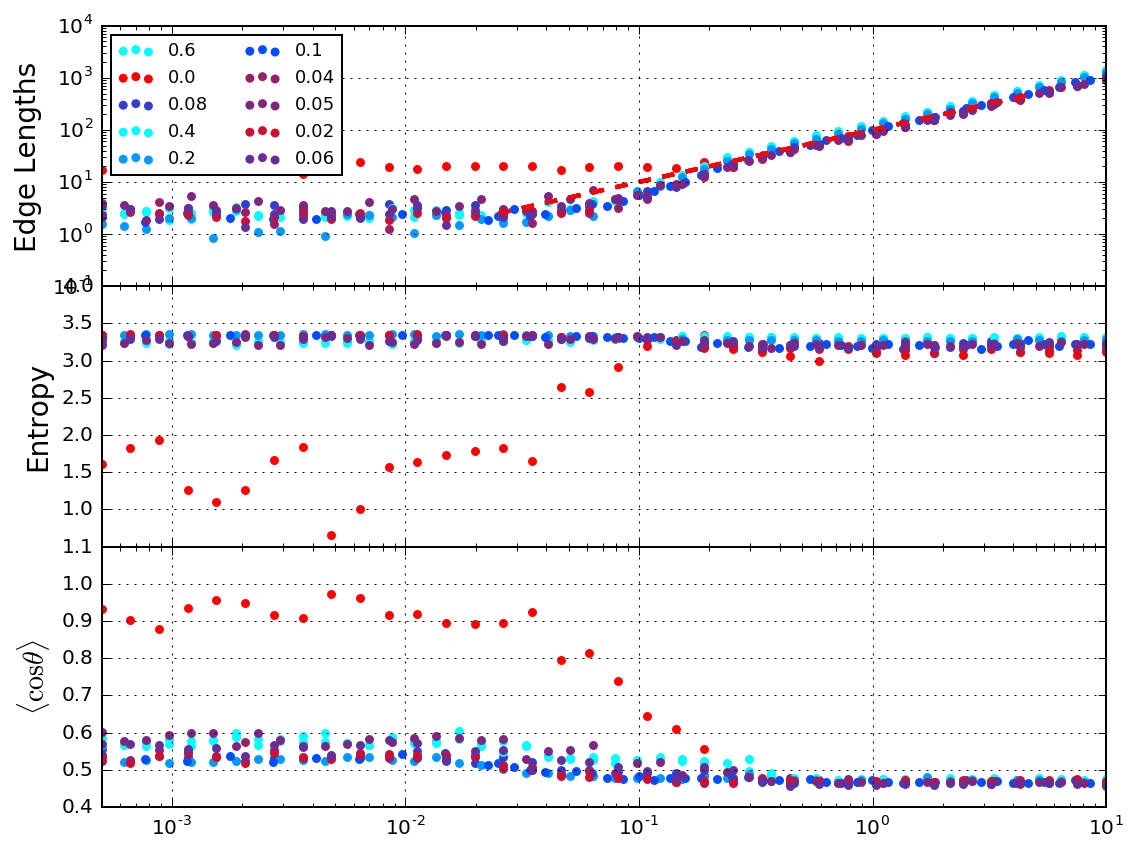
\includegraphics[width = \columnwidth]{fig-09-19/phase-ws}
    \caption{WS with different rewiring probabilities.}
    \label{fig:phase-ws}
\end{figure}
} %%%%


\outNim{
\begin{figure}
    \centering
    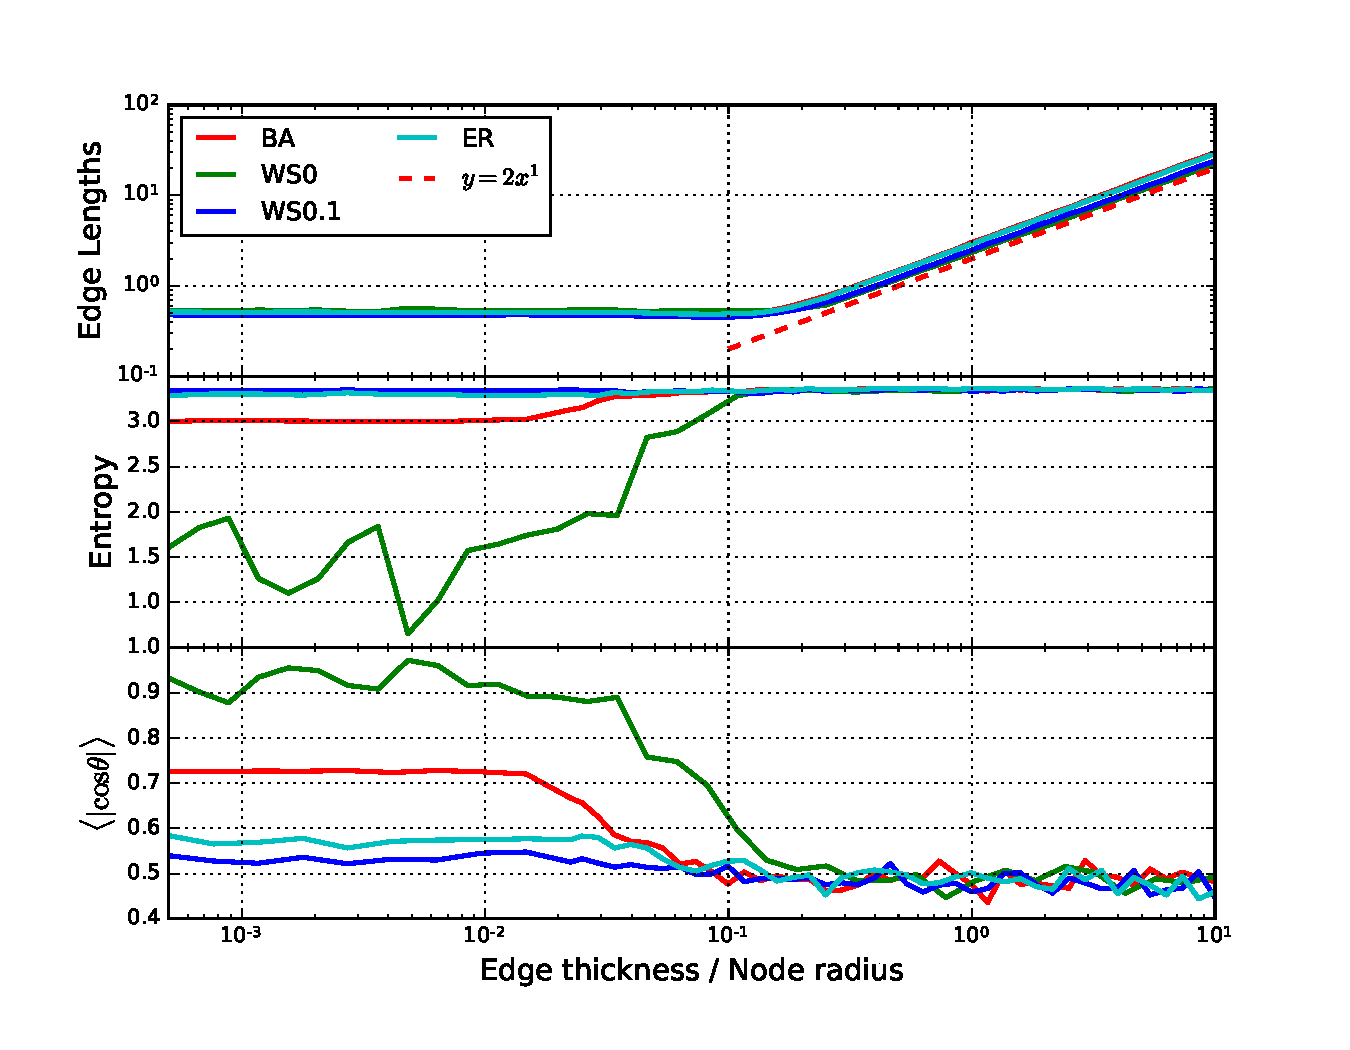
\includegraphics[width=\columnwidth]{fig-09-19/phase-topol.pdf}%phase-eman-all}
    \caption{Comparison of different network topologies. All networks have $N=49$ and $N_e\approx 280$. BA: Barabasi-Albert, ER: Erdős-Renyi; WS0.1: 2D Watts-Strogatz with rewiring probability $p=0.1$; WS0: without rewiring (only with local connections and no small-world property). The top plot shows the average link length. Surprisingly, the average link length is almost identical in all these networks. They all exhibit two phases: one where link length is almost remains constant, happening when links are thin compared to node exclusion radius; and one where average link length grows linearly, suggesting that the layout grows isometrically with the radius. The second plot shows the entropy $S =\sum_n p_n \log p_n$ of the distribution $p_n$ of $\cos\theta$ for angles of segments of eges that touch each other.  }
    \label{fig:phase-topol}
\end{figure}
}%%%


\outNim{\color{red}
\textit{Phase transition}. The way links organize depends on the space available for each link. The average length of the links $\langle l\rangle$ is of the order of the network size $R$, combining this with the thickness $r_l$ we get a volume of the order 
$V \sim r_l^2 \langle l \rangle \sim r_l^2 L. $
Thus the maximum thickness $r_{\mathrm{max}}$ would be 
$$ r_{\mathrm{max}} \approx \frac{L}{\sqrt{L}}$$
where $R$ is the side of the cube that would engulf the network and $L$ is the number of links. Since all links won't organize in parallel, the above condition is a lower-bound on the maximum thickness for which avoiding link crossing should be possible. In practice this yields only the order of magnitude of where we expect a phase transition.

}%%%



\outNim{
\section{Intuition}
In which of the regions should we expect to see the higher brains? Primitive brains have no spatial constraints, especially in non-vertebrates. Now consider the brain of a mammal. The size of the skull is often correlated with the size of the brain. In most animals, it is the cerebellum that contains most of the neurons, unlike human where there are more neurons in the cerebral cortex. 
The growth of the brain and its constraints can be tricky. The skull does not harden completely until most neurons have proliferated and even after neurons stop proliferating, the glia and the brain as a whole grows over time to a few times its original volume throughout the time the animal grows. 
What constraints does that impose? It is not an infinite pressure barrier, but it is also not a free space to roam in. The walls exert a small pressure. The system will have almost minimal volume. The layout of the brain in mammals and birds differ. Birds
do not seem to possess a distinct white matter. Can the restrictions push the system to be at a specific point on the phase diagram? The links will optimize their length as the brain grows. Their thickness will not necessarily fill the volume of the brain. 


\section{Interpretation}
In a biological context, a network scaffolding inside cells, chromatin, or brain cells will generally be inside a container, be it the cell, nucleus, or the skull. None of these containers is completely rigid and in the time-scale of their development, even the skull can thought of as a soft, though somewhat restraining, environment. 

Where would networks inside such soft constraining containers be in our phase space? The container doesn't fully restrict the growth, but it doesn't allow non-economical use of space. How do we quantify this? The container certainly exerts a pressure when the network grows larger. But instead of the pressure growing as the network grows, the container grows with it and it may be exerting a constant pressure on the network. Since elements of the network are elastically repelling each other, to first order the pressure it will exert grows linearly with push in one direction. If the thickness of fibers was growing in the network, they  
} %% outnim


\newpage

%\end{document}

\appendix
{\Huge Supporting Information}
% \setcounter{figure}{0}
% \renewcommand{\thefigure}{SI.\arabic{figure}}

\section{Contractible repelling links with self-repulsion\label{ap:ell}}
Note the $l\ne m $ in \eqref{eq:Vfull} in the link repulsion $V_{LL}$, excluding self-repulsion in links. 
The reason is $V_{LL}$ is modeling every link segment $ds_l$ as a soft sphere repelling other link segments in its vicinity.
Thus, allowing self-repulsion would interfere with contraction of elastic links and result in wiring length exceeding minimal possible length. 
While in most situations avoiding such self-repulsion is desired, in some cases where space is very limited links are pressed against themselves, bending sharply onto themselves as a consequence, and resulting in unnatural layouts. 
For these situations we propose a more sophisticated potential energy which models the link segments $ds_l$ as ellipsoids. 
These ellipsoids will have radii $r_L$ in directions perpendicular to the link segment and radius $|ds_l|/2$ along the link. 
$V_{LL}$ will then describe the interaction of pairs of ellipsoids, which can be achieved by replacing the simple Euclidean norm $|x_l-x_m|%\sqrt{(x_l-x_m)^T(x_l-x_m)} 
$ by a norm calculated using a ``double-ellipsoidal metric'' $\sqrt{\Delta x_{lm}^Tg^{(lm)}\Delta x_{lm}}$, where $\Delta x_{lm} = x_l-x_m$ (SI sec.\ref{ap:ell}). 
For a pair of link segments $ds_l$ and $ds_m$ this metric is given by 
\begin{align}
    g^{(lm)} = \left[\pr{r^{(l)}{R^{(l)}}^T+ r^{(m)}{R^{(m)}}^T} \pr{R^{(l)}{r^{(l)}}^T+ R^{(m)}{r^{(m)}}^T} \right]^{-1}
    \label{eq:g-ell}
\end{align}
where $r^{(l)} = \left(\begin{array}{c|c|c}{ds_l\over2} & r_{1} &r_{2}\end{array}
    \right)$ 
is the ``structure matrix'' of ellipsoid $l$, which is the set of three vectors defining the axes of the ellipsoid (one along the link segment $dsl/2$, and $r_1, r_2$ perpendicular to $ds_l$) and $R^{(l)}$ is the rotation matrix transforming these three vectors into the principal $x,y,z$ directions in space. 
The interaction of ellipsoids has been discussed extensively in the context of polymers and the Gay-Berne potential \citep{gay1981modification,berne1972gaussian,everaers2003interaction}. 
It has also been used to describe DNA and other macromolecules as stack of ellipsoids \citep{babadi2006coarse,mergell2003modeling,cleaver1996extension}.
The only difference in our case is that the ellipsoids will stretch and shrink with the links. 
Using this more accurate double-ellipsoid $V_{LL}$ and allowing $l=m$, resolves the anomalies in the case where space is limited (Fig. \ref{fig:ell}). 
Finally, note that the outcome of the ellipsoidal potential is the same as the spherical case when space is not limited as both models are minimizing wiring length, while avoiding crossings, and both have short-range repulsive forces.  
Thus we will use the spherically symmetric potential in \eqref{eq:Vfull} in most cases, unless space is too limited and the layout becomes unnatural. 
\begin{figure}
    \centering
    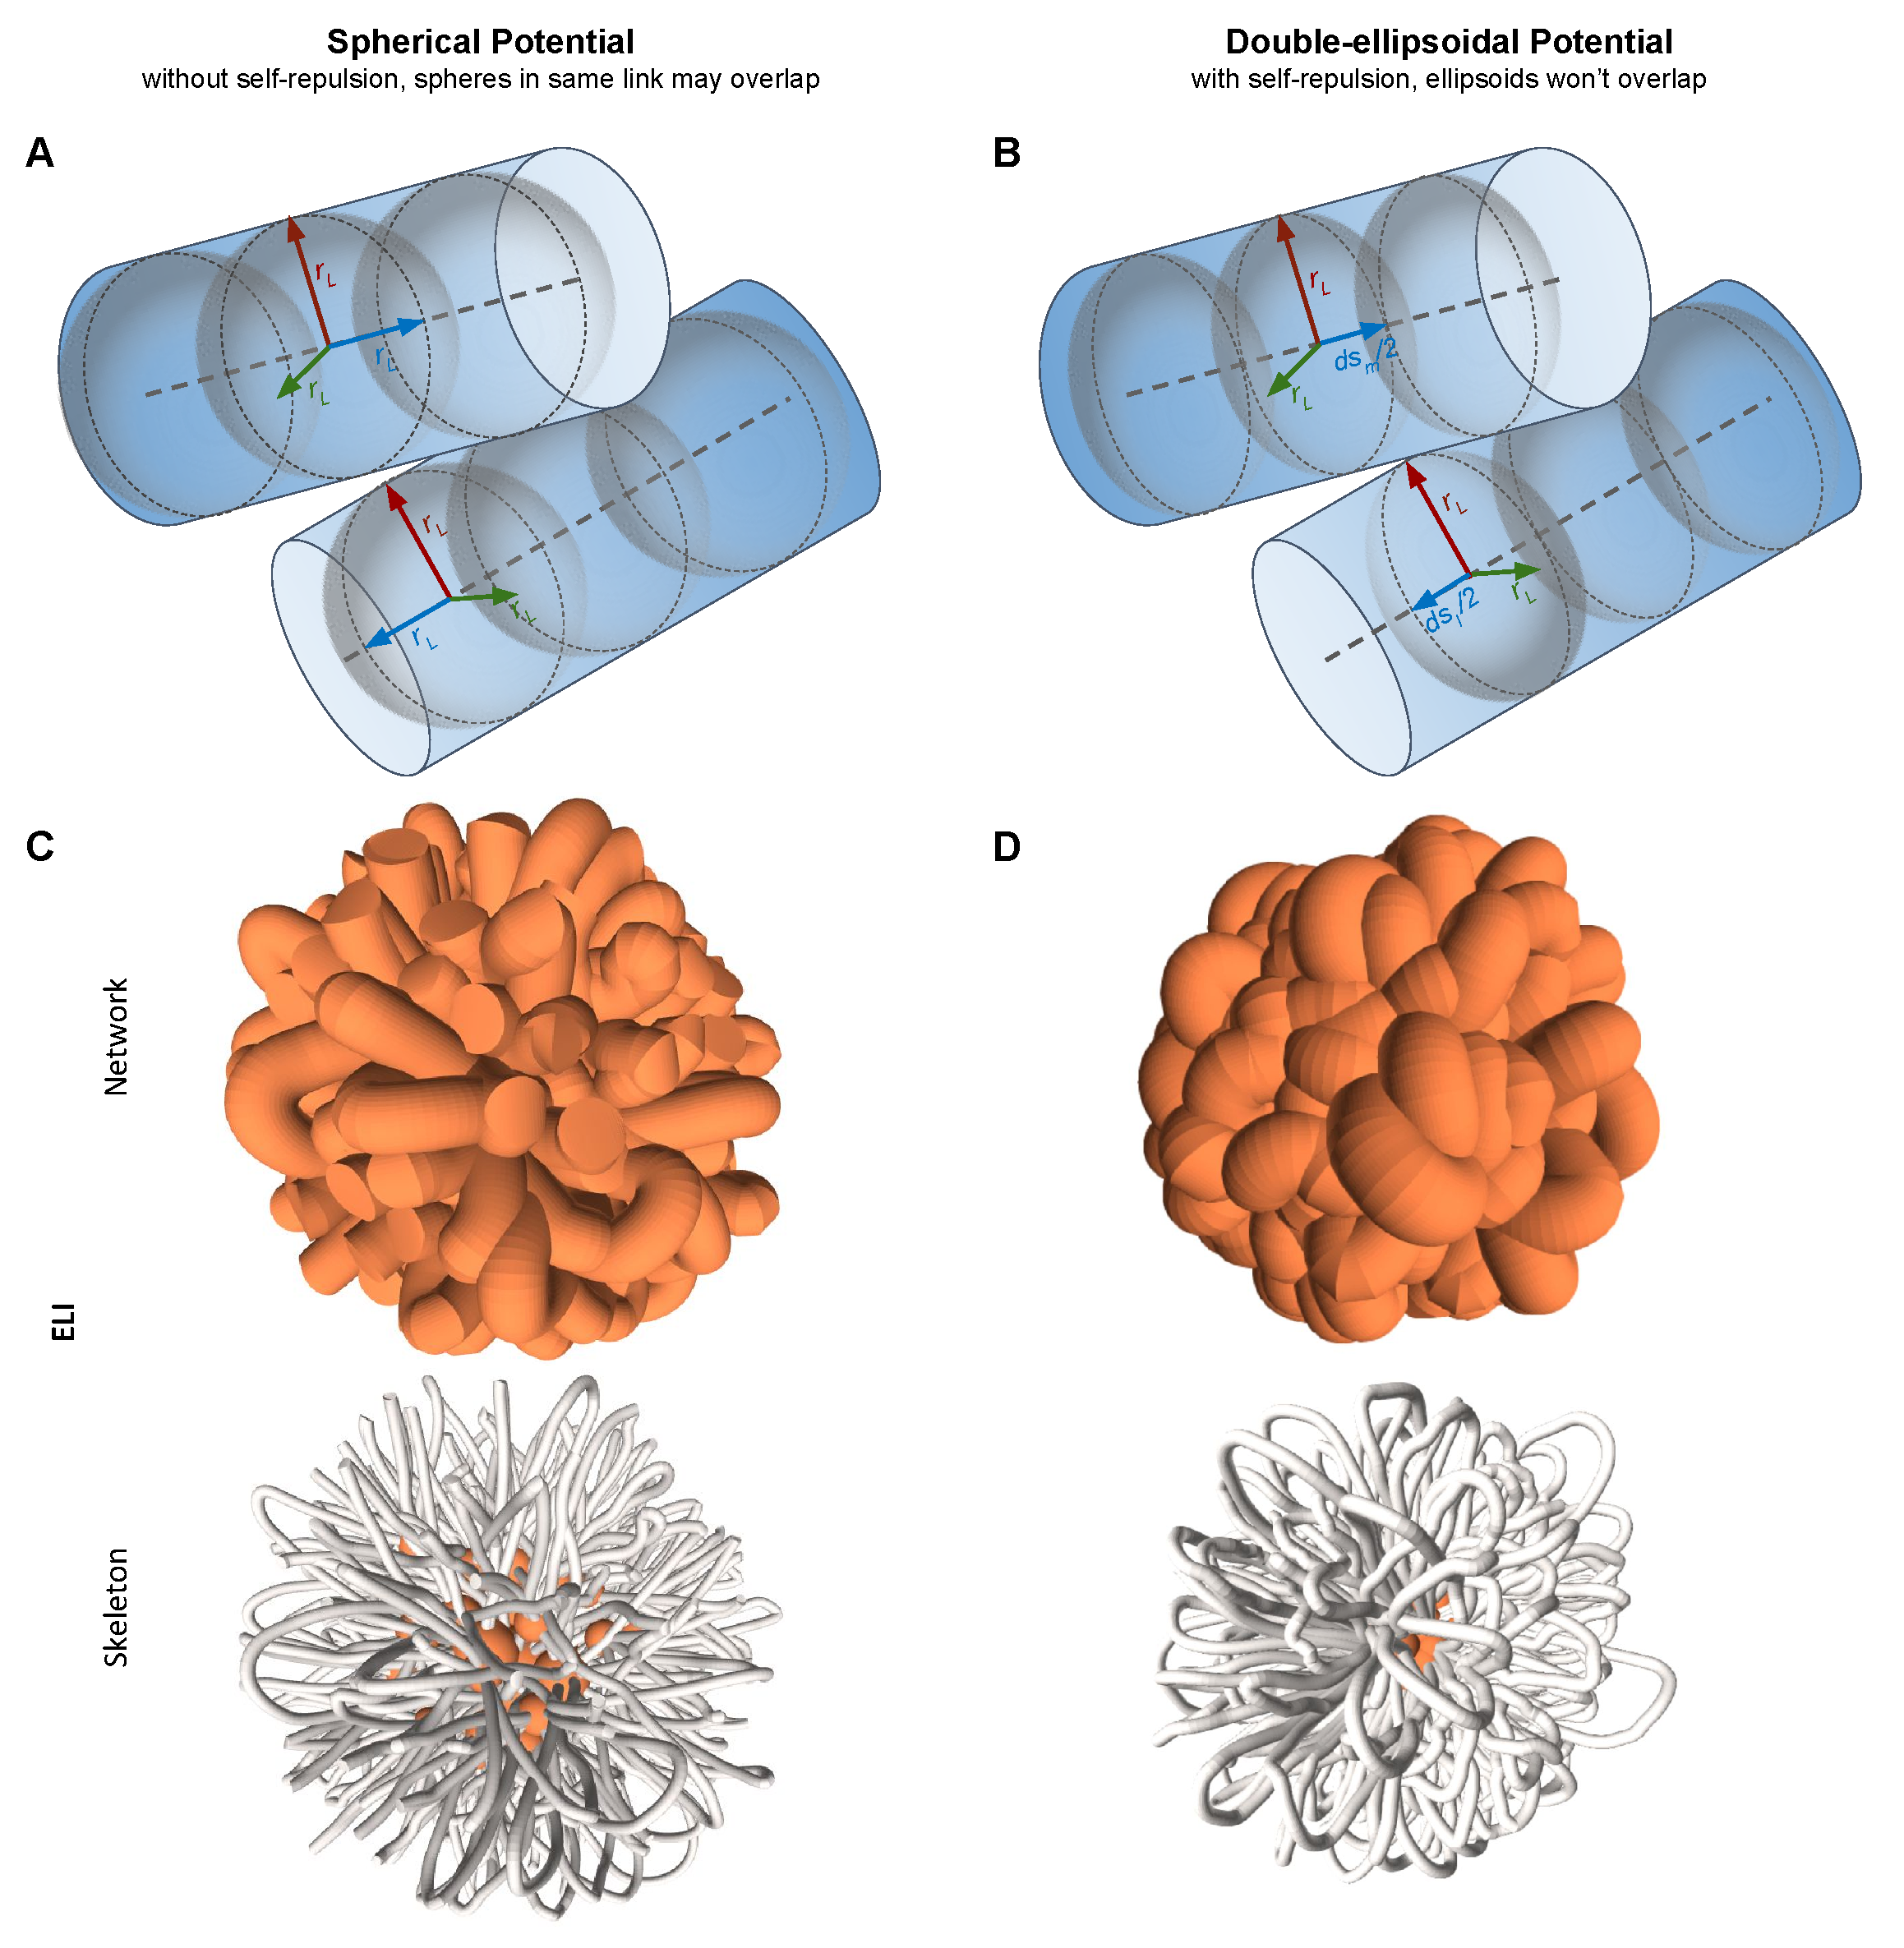
\includegraphics[width = \columnwidth]{fig-09-19/ellipsoid.pdf}
    \caption{\scriptsize{\bf Spherical vs Double-Ellipsoidal Potential:} If the forces between links $l,m$ depend on the Euclidean distance between link segments,
    it is as if each link segment generates a spherically symmetric potential around it and the overlap of these potential fields defines the interactions {\bf(A)}. 
    We must exclude self-repulsion within links in this case if we want the links to shrink to their minimal lengths.  
    Excluding self-repulsion is not an issue as long as no link is pushed against itself. 
    However, it poses a problem when space is very limited, for instance when nodes are fixed and links are very thick {\bf(C)}. 
    Lack of self-repulsion removes the penalty for links bending into themselves, resulting in sharp cusps and unnatural layouts.  
    We resolve this issue by using a more sophisticated potential field in link segments, and including self-repulsion. 
    If instead of a spherical potential field, each segments emanates a field which stretches and shrinks together with the link, we can make sure that the link segments of the same link exclude each other, while at the same time allowing the link to shrink to its minimal length.
    thus we define an ellipsoidal field stretching half the segment length $ds_l/2$ along the link $l$ and $r_L$ in the cross-section of the link {\bf(B)}. 
    The potential energy, then, arises from overlap of two ellipsoidal potential fields of a pair of links $l$ and $m$. {\bf(D)} shows the same network as in {\bf(C)} but this time using the double-ellipsoidal potential. 
    Notice the smooth nature of the layout in {\bf(D)} and the absence of the sharp ends resulting from self-crossing in {\bf(C)}.  
    }
    \label{fig:ell}
\end{figure}

\subsection{Motivation and Mathematical Derivation of the Double-ellipsoidal Metric}
When defining repulsive forces for elastic links, we are faced with a dilemma. 
Consider a simple short-range repulsive force, such as hard-core repulsion or smooth versions of it. 
They all define a minimum distance that any given point on a link would have from all other link points. 
Here lies the dilemma: 
On the one hand, we want the links to not have a predefined minimum length --the length is determined by the optimization process--, but on the other hand, we don't want a link to cross itself, either. 
If we introduce self-repulsion through a fixed radius hard-core repulsion, that radius times the number of discrete link segments determines the minimum link length and it will prevent us from finding optimal wiring length. 
The resolution that we propose is a repulsive force that adjusts itself to the length of the link. 

In directions perpendicular to the link segment, we want the range of the repulsive force to be the link thickness $r_L$. But along the link segment with length $ds$, we want the force to only reach a distance $ds/2$. 
This makes sure that the segment does not push its adjacent segments away and, thus, doesn't interfere with the link shrinking process, which is essential in the wiring length optimization.
To do so requires defining a much more complex type of force than spherical repulsion. 
We need to define a force based on the interaction of two ellipsoidal force fields. 
We call this the ``double-ellipsoidal'' basis, and it will require defining a metric for every pair of interacting link segments to measure how close they are relative to the link orientation, segment length and the link thickness. 
%The mathematical derivation of this is given in the SI sec.\ref{ap:ell}. 
The general idea is that the distance $\Delta x_{lm} = x_l(s_l) - x_m(s_m)$ between two link segments on links $l$ and $m$ is vector which in each direction need to be compared to how close the ellipsoids defined along the links $l$ and $m$ are to each other. 


\subsection{Double-Ellipsoidal Metric }
The current form of the repulsive force between two links $i,j$ is a function of the distance between points $x_i$ and $x_j$ along the links. 
Defining a distance requires defining a metric. 
Naively, one might think that this metric is the euclidean space metric, but note that the strength of the force depends on the scale defined in this metric. 
For instance, in the Gaussian potential for links with thickness $r_L$ the width of the Gaussian can be thought of as part of the metric function $g(X,Y)$. 
In other words, the metric yields
\[g(\Delta x, \Delta x) = \Delta x^i \Delta x^j {\delta_{ij} \over (2 r_L)^2}  \]
The denominator comes from he thickness of the two links. When the thicknesses are different, we must have
\[g(\Delta x, \Delta x) = \Delta x^i \Delta x^j {\delta_{ij} \over ( r^{(i)} +r^{(j)})^2}  \]
To generalize this to the case of ellipsoidal potential, we must first understand how this metric relates to projections along different directions. 
The inverse of the metric can be related to these projections. 
We want a definition of the inverse metric which would yield $\pr{r^{(i)} +r^{(j)}}^2$ in the spherical case. 

The inverse metric is defined on the tangent space as a symmetric rank 2 tensor $ g^{-1} = \pr{g^{-1}}^{\mu\nu}\ro_\mu \ro_\nu $. 
The components of the inverse metric  come from three projections onto three vectors $v_i$
\begin{equation}
    \pr{g^{-1}}^{\mu\nu} = V^\mu_\rho \delta^{\rho \lambda} V^\nu_\lambda =  \sum_{\rho} V_\rho^\mu V_\rho^\nu \label{eq:ginv}
\end{equation}
For each pair of links $i,j$ if we define the vectors as $V_\rho^\mu =% \vec{r}_{1i}+\vec{r}_{2i} = 
\pr{{r^{(i)}}_{\rho}^\mu+{r^{(j)}}_{\rho}^\mu} $. 
$r^{(i)}$ and $r^{(j)}$ are each a set of three mutually orthogonal vectors defining the axes of the ellipsoids. 
When we have spheres, all three vectors $r^{(i)}_\rho$ and $r^{(i)}_\rho$ have the same magnitude. 
The spherical case should reduce to the usual metric with the radii $r^{(1)}$ and $r^{(2)}$ of the spheres appearing in the metric along the diagonal, as 
%In this case, we can choose the three vectors $r^{(1)}_{\rho } + r^{(2)}_{\rho}$ always have the same projection in all directions and so 

$$ \pr{g^{-1}}^{\mu\nu} = |r^{(i)}+r^{(j)}|\sum_{\rho} \hat{r}_\rho^\mu \hat{r}_\rho^\nu = |r^{(1)}+r^{(2)}| \delta^{\mu\nu }$$
This is because $ \pr{g^{-1}}^{\mu\nu} $ is a Hermitian matrix with all eigenvalues equal to $|r^{(1)}+r^{(2)}|$ and is therefore proportional to the identity matrix $I$. The identity matrix is invariant under all rotations and so, this metric is diagonal in all bases.
We will use this as a test for the consistency of our double-ellipsoidal metric below. 
 
\subsection{Different Orientations}
We start by defining what we will call the ``orientation tensor'' of the ellipsoid. 
This tensor is the set of vectors defining the major axes of the ellipsoid and in the orthonormal basis of the axes f the ellipsoid it becomes diagonal. Let us denote everything in the basis of the ellipsoid by a prime as $x',y',z'$. The orientation tensor in this basis is  
\begin{equation}
    {r'}^{(i)} = \left(\begin{array}{c|c|c}r'_{x'} & r'_{y'} &r'_{z'}\end{array}
    \right) = R \begin{pmatrix}
    |r'_{x'}| \\ 
    & |r'_{y'}|\\ 
    & &|r'_{z'}|
    \end{pmatrix}
    \label{eq:ell}
\end{equation}
%What happens if the vectors defining the ellipsoids of the two links are not along the principal directions (i.e. $x,y,z$)? 
The set of orientation vectors $r^{(i)}$ with components ${r^{(i)}}_{\mu}^\nu$ is a (1,1) tensor and transforms under rotations $R$ as $r \to R^{-1} r R$. 
For the spherical case, this doesn't matter, because the orientation tensor $r^{(i)} = |r|I$ and is invariant under rotations. 
But other cases where the ellipsoid has different radii in different directions require us to find the transformations that take a diagonal $r = \mathrm{diag}(r_x,r_y,r_z)$ from the basis of the ellipsoid to the global $x,y,z$. 
In practice, we know the axes of the ellipsoid in the global coordinates as three vectors with components  ${r^{(i)}}_{x'}^\mu, {r^{(i)}}_{y'}^\mu, {r^{(i)}}_{z'}^\mu$ with $\mu = x,y,z$ of the global coordinates. However, the other index $x',y',z'$ is defined in the basis of the ellipsoid and we still need to transform that index to the global coordinates.  
To reiterate,  we have the three columns of $r^{(i)}$ as vectors in the global coordinates $\mu$, we already have the row index transformed into the global basis and don't need to transform it again. 
But we do need to transform the ellipsoid $\mu'$ index, which involves a rotation similar to the rotation that would act on $r^{(i)}$ to take the $\mu$ index to the local $\mu'$, just transposed. 
How do we efficiently find this transformation? 
To do this, note that $r^{(i)}$ is the result of acting with one rotation $R$ from the one side on a diagonal matrix with the radii of the ellipsoid $r'_{\mu'}$ on its diagonal, that is
\begin{equation}
    r^{(i)} = \left(\begin{array}{c|c|c}r'_{x'} & r'_{y'} &r'_{z'}\end{array}
    \right) = R \begin{pmatrix}
    |r'_{x'}| \\ 
    & |r'_{y'}|\\ 
    & &|r'_{z'}|
    \end{pmatrix}
\end{equation}
Thus, if we Find the magnitude of each column and divide the column by it, we find $R$. 
Then we simply multiply $r^{(i)}$ by the transpose of $R$ from the right in order to go from the $\mu'$ basis to the global $\mu$ basis 
\[\tilde{r}^{(i)} = r^{(i)}R^T. \]
$\tilde{r}^{(i)}$ has components $\pr{{\tilde{r}^{(i)}}}^\mu_\nu$ where both indices are in the global coordinates.
Note that this step is crucial when dealing with two ellipsoids with different orientations, because, although \eqref{eq:ginv} has an inner product on the local index $\rho$, the basis in which $r^{(i)}$ and $r^{(j)}$ are diagonal are the orientation bases of each of the ellipsoids they represent. 
Therefore, both have to be first transformed into a similar basis (e.g. the global basis) before they can be added in $V^{\mu}_\rho$. 
Once we have these transformed orientation vectors, the inverse metric 
It is easy to check that for a sphere $\tilde{r}^{(i)}$ is diagonal and thus the inverse metric remains a scaled Euclidean metric. 
Thus, the final step is to combine the transformed orientation tensors and construct the metric for the pair $i,j$ as 
\begin{equation}
    g_{\mu\nu}^{(ij)} = \left[\pr{r^{(i)}{R^{(i)}}^T+ r^{(j)}{R^{(j)}}^T} \pr{R^{(i)}{r^{(i)}}^T+ R^{(j)}{r^{(j)}}^T} \right]^{-1}_{\mu\nu}
\end{equation}
The potential energy is then defined similar to befor, only this time using the new metric 
\begin{align}
    \Delta {x^{(ij)}} &= x^{(i)} - x^{(j)}\cr
    V_{ij} &= A\exp\left[\pr{
    g_{\mu\nu}^{(ij)} \Delta {x^{(ij)}}^\mu \Delta {x^{(ij)}}^\nu }^{p/2}   \right]
    %\cr f(x) &= A \exp\left[- x^p \right]
    \label{eq:Vij-ell}
\end{align}
where sum over $\mu,\nu$ is understood (i.e Einstein notation).

\subsection{Implementation}
To construct the ellipsoids, we first need to find two vectors perpendicular to the $dl$ vector going along the link segment. This can be done using the cross product.
For example, the two vectors can be found through 
\begin{equation}
    \hat{r}_1 = \hat{x} \times \hat{dl}, \quad \hat{r}_2 = \hat{r}_1 \times \hat{dl} 
    \label{eq:r12}
\end{equation}
and then define $r_1 = r_L \hat{r}_1$ and $r_2 = r_L \hat{r}_2$. Finally, to ensure that the cross product in $\hat{r}_1$ doesn't vanish, instead of $\hat{x}$ we should choose the direction in which $dl$ has the smallest projection. 
In terms of time complexity, brute-force matrix inversion is $O(n^3)$ and the dot product using the metric is $O(n^2)$, while the spherical case had a simple dot product for $|\Delta x|$, which is $O(n)$. Here $n=3$ is the dimensions of the vectors. 
However, the main part of the time complexity comes from iterating over $N_s$ different link segment points and forming interaction pairs. 
Since that part is not different between using the spherical versus Ellipsoidal forces, the overall complexity only changes by a factor, and the exponent of $N_s$ will not change.


\section{Curvature\label{ap:curvature}}
The curvature of a curve $\gamma(s)$ measures how much the tangent of the curve $T(s) \equiv \gamma'(s)$ changes along the path. 
Here $s$ is an affine parameter, like the arc-length.  
Hence, the extrinsic curvature $\kappa(s)$ is given by magnitude of the second derivative of the curve 
\begin{equation}
    \kappa(s) = |T'(s)| = |\gamma''(s)|
\end{equation}
The path is defined as $\gamma(s) = (x(s),y(s),z(s))$ in Cartesian coordinates and the tangent related to the gradient of $\gamma(s)$
\begin{align}
    T(s) &= {d \gamma(s) \over ds} = \vec{x}'(s)\cdot \vec{\del} \gamma(s) = x'(s)\hat{x}+y'(s)\hat{y}+z'(s)\hat{z} 
\end{align}
Since $s$ is the affine parameter and $ds^2 = dx^2 + dy^2 + dz^2$, we always have $|T(s)|=1$. 
For arbitrary parametrization, we have $T = \gamma'/|\gamma'|$.
Therefore, just as in circular motion, $T'(s)$ will be perpendicular to $T(s)$ and related to the radius of curvature. 
Taking the second derivative, the curvature can be summarized as 
\begin{equation}
    \kappa = {|\gamma'\times \gamma''|\over |\gamma'|^{3}}
\end{equation}
\begin{figure}
    \centering
    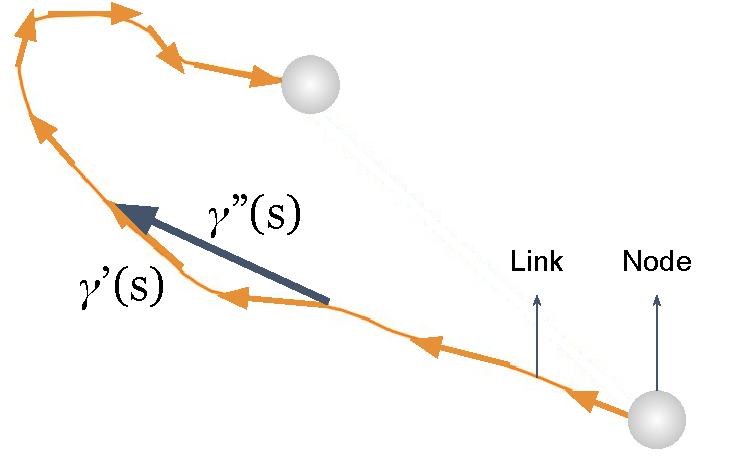
\includegraphics[width = .5\columnwidth]{fig-09-19/curvature.pdf}
    \caption{Link curvature, which is equal to the inverse of the radius of curvature, is related to the angle between the tangent vector $\gamma'(s)$ and the change in the tangent vector $\gamma''(s)$. This can be estimated discretely in numerical simulations.}
    \label{fig:curvature}
\end{figure}
In practice, for measuring link curvature, we can implement this by measuring the cross product of the tangent vector $\gamma'(s)$, calculated for every link segment, and the second derivative $\gamma''(s)$ and dividing by $|\gamma'(s)|^3$. 
Note that $\kappa(s) = 1/R(s)$ with $R(s)$ being the radius of curvature. 
But, taking the same curve and scaling it up will increase the radius of curvature and decrease the curvature. 
Therefore, to compare curvature in networks of various sizes we rescale the curvature by the average link length $\be{l}$ and measure $\be{l}\kappa(s) = \be{l}/R(s)$.


\section{Stress Tensor\label{ap:stress}}


To understand how ELI and FUEL respond to stress we must analyze various components of their ``Cauchy stress tensor''. 

Consider moving one of a node or a point on a link at position $x$ by a small amount $\delta \vec{x}$.
The network will respond to the change with a force, which to lowest order in $\delta \vec{x}$ is given by
\begin{equation}
\vec{F} (\vec{x}+\delta \vec{x}) \approx %\vec{F} (\vec{x})+\delta \vec{x}\cdot  \vec{\del} \vec{F} (\vec{x}) = 
\vec{F} (\vec{x})-\delta \vec{x}\cdot  \vec{\del} \pr{\vec{\del} v (\vec{x})}.\label{eq:dF}    
\end{equation}
Where $v(x)$ is the potential energy density and the full potential energy $V$ is $V = \int_\mathrm{Net} d^3x v(x)$. 
The term $-\vec{\del} \pr{\vec{\del} v (\vec{x})}$ is the Cauchy stress tensor and has components $T_{\mu\nu}(\vec{x}) \equiv -\ro_\mu\ro_\nu v(\vec{x})$, with $\mu$ and $\nu$ labeling $(x,y,z)$ components. 
Note that $v,F_\mu,T_{\mu\nu}$ are all densities. 
To get the total potential energy, force and stress we need to integrate over the volume of the space. 

In terms of components, we need the Hessian matrix of the potential energy
\begin{align}
    T_{\mu\nu}(x) =&  %\ro_\mu \ro_\nu V(x) =& 
    \ro_\mu \ro_\nu \pr{V_{el}+V_{LL} + V_{NN}+V_{NL}} \cr
    =& k \delta_{\mu\nu}\int dl \sum_l \delta^3(x-x_l(l)) \cr
    &+ 
    \sum_{l\ne m} \iint ds_l ds_m \delta^3(x-x_l(s_l))\frac{-4r_L^2\delta_{\mu\nu}+ x_{ab\mu} x_{lm\nu}}{16r_L^4}
    A \exp\left[- {|r_{lm}|^2 \over 4 r_L^2}\right]\cr
    &+ \sum_{i\ne j}\delta(x-X_i)\frac{-4r_N^2\delta_{\mu\nu}+ X_{ij\mu}X_{ij\nu}}{16r_N^4}
    A \exp\left[- {|\vec{X}_{ij}|^2 \over 4 r_N^2}\right]
    \label{eq:T}
\end{align}
where $\vec{x}_{lm} \equiv \vec{x}_l-\vec{x}_m$ and $\vec{X}_{ij} \equiv \vec{X}_i-\vec{X}_j$. The first row corresponds to the elastic stress in the links, the second to the link repulsion and the third to node forces\footnote{
Note that the first term contains both the elastic forces and the node-link forces, as they are just the elastic forces at link end-points.}. 
In the strong exclusion phase the links that touch each other will all be at distance $2\be{r}$ where the average distance is found as follows. The cross-section of links is 2D, so vectors $r = r_{ab}$ run in 2D. 
\begin{align}
b &\equiv \pr{4r_L^2}^{-1}\cr
C &= \int d^2 r e^{-br^2} = {\pi\over b} = 4\pi r_L^2 \cr
\be{r} &= C^{-1}\int r d^2 r e^{-br^2} = - 2\pi C^{-1}\ro_m \sqrt{{\pi\over b}} \cr &= C^{-1} \pr{{\pi\over b}}^{3/2}    = {8\pi^{3/2} r_L^3\over 4 \pi r_L^2} = 2\sqrt{\pi} r_L \cr
\be{r^2} &= C^{-1}\int r^2 d^2 r e^{-b r^2} = - C^{-1}\ro_m C = 4r_L^2.
\end{align}
For links that touch each other $|r_{ab}| \approx \be{r}$. Since in the strong exclusion phase the links fill up the space, each link is approximately covered by other links along its entire length. This means that the sum over adjacent links basically defines an envelope which covers the link. 
The sum over $b$ also becomes an integral over all directions for $\vec{x}_{ab}$ because the link is covered on all sides. Writing $\vec{x}_{ab} \approx  \be{r}\hat{n}$ we get 
\begin{align}
    \sum_{b\ne a} \iint ds_lds_m f(\vec{x}_{ab}) &  \approx \int d\hat{n} f(\be{r}\hat{n})\int s_l ds_l\cr 
    & = {1\over 2} \be{l^2}\int d\hat{n} f(\be{r}\hat{n}).
\end{align}
Also, note that 
\begin{equation}
\int d\hat{n} n_\mu n_\nu = \delta_{\mu\nu}    
\end{equation}
This can, for example, be seen by writing $\hat{n}$ in the 2D cross-sectional plane of each point on the link in 
in polar coordinates. In this plane $d\hat{n} = d\theta $ and  the $x,y$ components in this plane become
\begin{align}
    \int d\hat{n} n_x n_x & = 
    \int d\theta \cos^2 \theta = {1\over 2} \cr
    \int d\hat{n} n_x n_y & = \int d\theta \sin \theta \cos \theta = 0 \cr 
    \Rightarrow  \int d\hat{n} n_\mu n_\nu & = {L\over 2} \delta_{\mu\nu} 
\end{align}
This result is valid in higher dimensions as well, as using spherical and generalized polar coordinates easily show. 
Thus, integrating over the whole space, to get total   link-link stress contribution in the strong phase, we get
\begin{align}
    \int d^3x \ro_\mu\ro_\nu V_{LL}(x) & \approx {4r_L^2 e^{-\be{r}/(4r_L^2)}\over 16r_L^4} \int s_l ds_l  \pr{-\delta_{\mu\nu} + {\be{r}^2\over 4r_L^2} \int d\hat{n} n_\mu n_\nu }\cr
    & =  {L e^{-\be{r}/(4r_L^2)}\over 4r_L^2}  \pr{  {\be{r}^2\over 8r_L^2} -1  } \be{l}^2 \delta_{\mu\nu}\cr
    & =  {L e^{-\pi}\over 4r_L^2}  \pr{  {\pi\over 2} -1  } \be{l}^2 \delta_{\mu\nu} \label{eq:TLL}
\end{align}

The repulsive terms in \eqref{eq:T} resemble the pressure tensor discussed in \cite{stillinger1984packing} and used for describing jamming phenomena and stress networks in granular material  \cite{o2002random,o2003jamming}.  
Since the repulsive potentials keep links that touch each other at a distance of $2r_L$, we have $\vec{x}_{ab}\approx 2r_L \hat{x}_{ab}$ if $a$ and $b$ touch. 
Here $\hat{x}_{ab}$ is the unit vector of $\vec{x}_{ab}$.  
If they do not touch, the Gaussian part strongly suppresses the repulsive term. 
Same is true of the node repulsion $V_{NN}$, with nodes that feel each other's force being at a distance $|X_{ij}|\approx 2r_N$ and nodes farther apart than $2r_N$ basically not contributing to $T_{\mu\nu}$. 
\begin{figure}
    \centering
    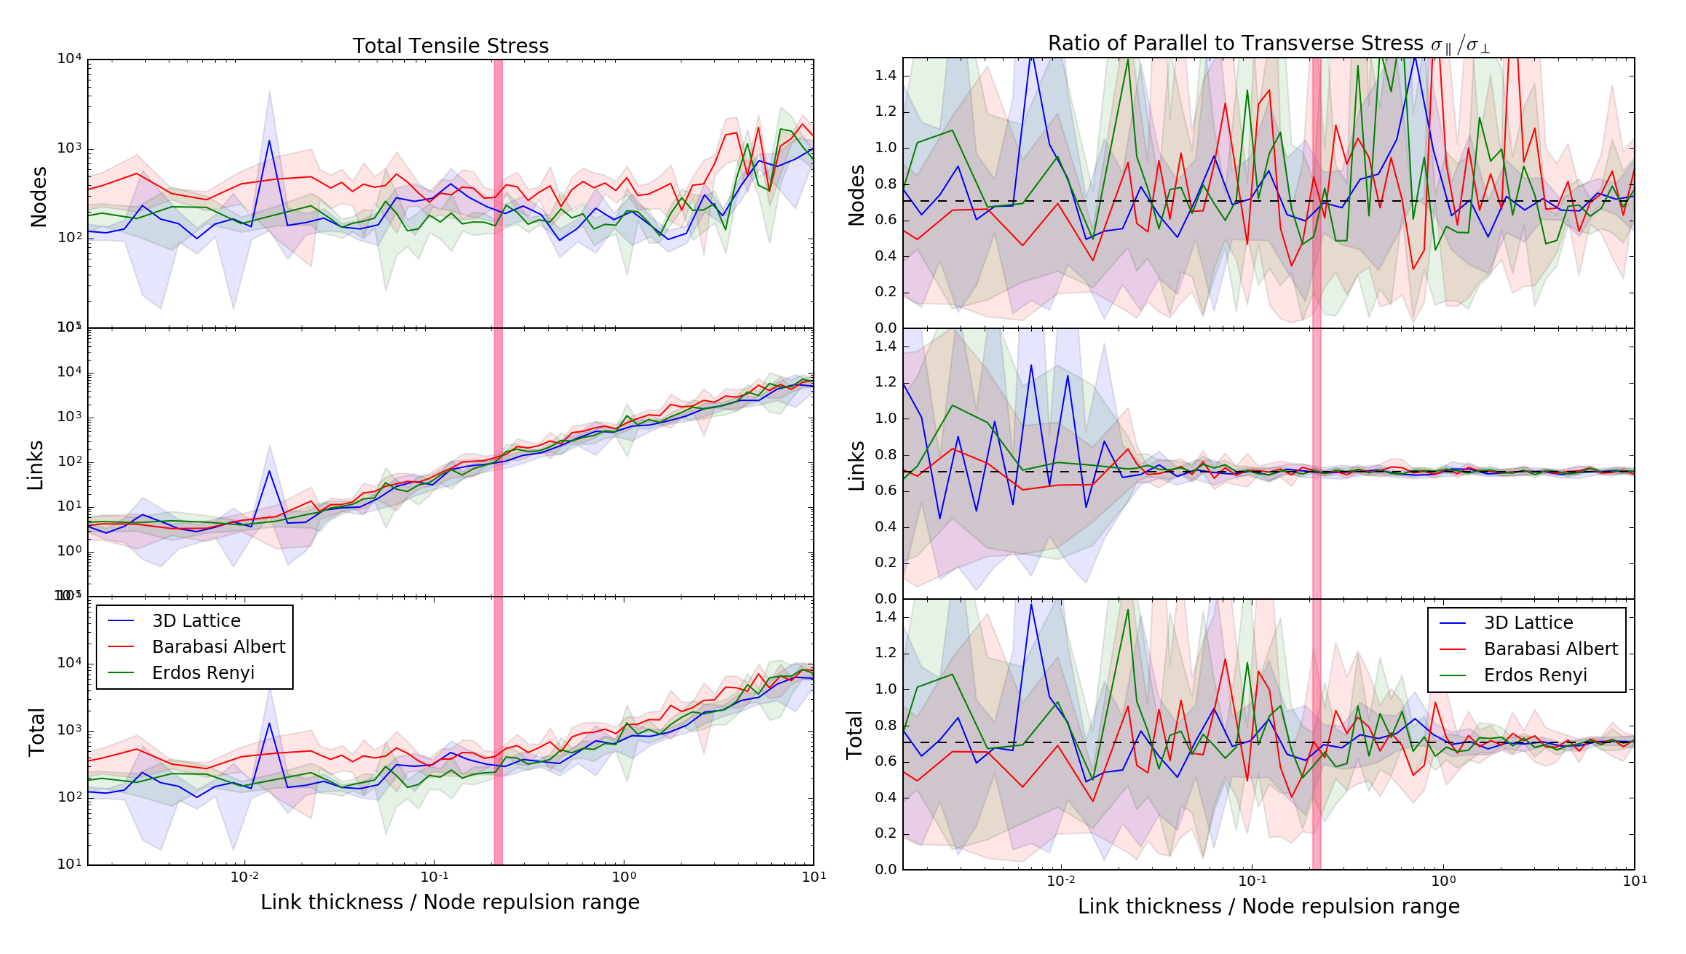
\includegraphics[width=1\columnwidth]{fig-09-19/stress3.png}
    \caption{Left: Total stress in an ER and a BA network with 49 nodes and 280 links, and a 3D lattice network with 300 links at various link thicknesses. 
    The solid curve is the average over 10 measurements done by randomly rotating the layout in space and the  shaded area shows one standard deviation around this average value. 
    The red strip indicates the approximate transition point.   
    Right: The ratio of parallel and transverse stress in BA, ER and 3D lattice. In the strong exclusion phase, the ratio becomes $1/\sqrt{2}$ (black dashed horizontal line) in  all three networks. 
    This indicates transition to hydrostatic stress, meaning that stress is uniformly distributed in all direction like a fluid. 
    The green strip indicates the transition point.}
    \label{fig:stress2}
\end{figure}
\outNim{

  

In the strong exclusion limit, the links fill up most of the space and nodes are more than $2r_N$ apart from each other, therefore $V_{NN} \sim 0$. 
In the final equilibrium most links are in contact with other links along their entire length. 
Consequently, 
we get 
%\begin{equation}
    $\sum_{<ab>}\int ds_l ds_m \hat{x}_{ab \mu} \hat{x}_{ab\nu} \sim  L\be{l^2} \delta_{\mu\nu}.$ 
%\end{equation}
where $<ab>$ means adjacent links, $L$ is the number of links and $\be{l^2}$ is the average square link length. 
The other term in $V_{LL}$ is
$\delta_{\mu\nu}\sum_{<ab>}\int ds_l ds_m \approx L \be{l}^2 $
Thus, in the strong exclusion phase the stress tensor is approximately
\begin{align}
    \int dx T_{\mu\nu} & \approx \delta_{\mu\nu} \pr{k + L Ae^{-1} {\sigma_l^2\over 4r_L^2} }
    \label{eq:Tstrong}
\end{align}
with $\sigma_l^2 = \be{l^2} - \be{l}^2$. 

} %%% outnim

We examined numerically whether the $ \sigma_\parallel/ \sigma_\perp$ ratio is constant in the ELI layouts.
We find that, as predicted by the theory, $\sigma_\parallel/\sigma_\perp$ fluctuates significantly for node stress at almost all (except at very high) link thicknesses, indicating that it does not satisfy the hydrostatic condition (Fig. \ref{fig:stress}D).%(SI sec.\ref{ap:stress}).
In contrast, the stress in links shows a remarkably constant  $\sigma_\parallel/\sigma_\perp$ ratio starting at thicknesses well below the phase transition, indicated by a red strip (SI). 
At very low thicknesses link stress too shows large fluctuations. 

\section{Initial Crossings and Total Volume\label{ap:cross}}
Before examining the bent links, we should first discuss the behavior of link crossing in the embedded network when the link are straight. Simulations using FR confirm that link crossings in this layout behave like random uniform layout of nodes in 3D. It is easy to prove that under such a distribution the number of link crossings grows linearly with link thickness\footnote{Assuming cylindrical links. % with circular cross-section.
}. A sketch helping understand the proof is in Fig. \ref{fig:crs1}. 
\begin{figure}
    \centering
    \includegraphics[width =.99\columnwidth]{figs2/{full-range-n100-m3}.pdf}
    \caption{Left: The behavior of the number of crossings as a function of link thickness. Trivially, once the thickness becomes comparable to the network size (when ``thickness/net. size'' becomes order 1) the crossings saturate and most links cross. The region in which trying to make links avoid each other is much smaller. It extends from zero thickness up to where thickness / net. size is of order $1/\sqrt{N_e}$ with $N_e$ being the number of links in the network. In the BA network with 100 nodes and $m=3$ considered here $1/\sqrt{N_3} \approx 0.06$, which is a safe lower limit for the region where avoiding crossings is possible. Right: a zoomed-in version of the dashed-red box on the lest highlighting this region of validity of avoiding crossings. The legends show a good linear fit to the data up to thickness / net. size = $0.2$.}
    \label{fig:full-range} 
\end{figure}

\begin{figure}
    \centering
    \includegraphics[width =.9\columnwidth]{figs2/crs1.png}
    \caption{\textbf{Left:} The projection of the line through the center of an link \textsf{\textbf{ e1}} on the plane normal to link \textsf{\textbf{ e2}} which crosses the link at point \textsf{\textbf{ n2}}. Because links are randomly oriented, the distance of \textsf{\textbf{ e1}} and \textsf{\textbf{ e2}} is the distance of the blue line from the point \textsf{\textbf{ n2}}. The uniformity then means that the blue lines have uniform density at random angles on the plane and thus their number within distance $d$ is linear in $d$. \textbf{Right:} If links were parallel, the projection of \textsf{\textbf{ e1}} onto the plane would be a point. Thus the distance of the links is the distance of two points on the plane. Uniform spatial distribution in this case means we get uniformly distributed points on the plane and their number within a circle of radius $d$ grows as $d^2$.}
    \label{fig:crs1}
\end{figure}


The key point is that the number of links within distance $r$ of a point on link $a$  can be found by projecting all links onto the plane to which link $a$ is normal. Since the angle distribution is random, we get a uniform distribution of lines on this plane and the number of lines within distance $r$ of a point on a 2D plane grows linear in $r$. 

Analyzing the number crossings as a function of link thickness in FR layout yield a linearly growing number of crossings\footnote{The exact properties of the point where the crossings start is not our primary concern here, but it seems to start at a certain nonzero thickness. 
This sharp phase transition is actually a feature of these connected networks with FR layout. The transition disappears, as expected, in a system of randomly oriented disconnected links in 3D. The length scale at which this phase transition occurs is a function of some dimensionful parameter that can naturally arise from the difference in the form of the repulsive node forces and the attractive forces on the links. We did experiment adding noise to the layout and also randomly switched links around. While these changes increased the slope of the line of the crossings (generally showing more crossings than FR) they did {\em not} move the point of the phase transition appreciably.}. 
 
As far as our goal is concerned, the point where crossings become noticeable seems to depend mostly on the network density parameters, similar to how in self-avoiding polymers the excluded volume depends on the interaction strength. 
After all, the nodes can be modeled as interaction points (vulcanization points) on a self-avoiding polymer.  

% \newpage
% \appendix

\subsection{Examining randomness of crossings}
For simiplicity, let's first consider a number of dots scattered with a random uniform distribution in $d$ dimensional space with a density $\rho$. Suppose we want to grow $d$ dimensional balls around these dots and wish to count the number of balls that overlap. Because of the uniformity, the total number of balls of radius $r$ crossing each other is the number of points that are within less than $2r$ distance of each other, which is
\begin{equation}
    n(r) = \int_0^{2r} \rho(r) dVol=\rho \Omega_{d-1} (2r)^d  \label{eq:nr}
\end{equation}
which scales with the volume of space. In two dimensions, for example, this would mean that the number of circles of radius $r$ crossing each other will be $4\pi \rho r^2$. To compare with the problem of link crossing, if we had parallel cylindrical links in 3d, their cross-section would have been randomly scattered circles in 2D and again the number of crossings should grow quadratically with radius. 

\begin{figure}
    \centering
    \includegraphics[width = .33\textwidth]{figs/para1dir.png}\includegraphics[width = .33\textwidth]{figs/phase-sim-parallel-200-regs-30.pdf}\includegraphics[width = .33\textwidth]{figs/phase-sim-parallel-200-regs-300.pdf}
    \caption{Simulated crossing count of 200 parallel links. One simulation used 30 partition cells in space and the other used 300 cells. In both the number of crossings grows as $r^2$, in accordance with the theoretical expectation. This is in contrast with the linear trend observed in the link crossing of force-directed layouts of random graphs.}
    \label{fig:simpara}
\end{figure}


Now consider infinite cylindrical links scattered with random orientations inside 3D space. Assume that the space occupied by the cylinders has a roughly constant density within cubes of links $d \gg r$. Take the cross-section of this space with a flat plane. The center lines of the cylinders become uniformly distributed points on the plane and the cross-section of the cylinders become ellipses. The ellipses may be very eccentric, but the minor axis, which is also the radius of the largest circle that fits inside the ellipse, is again $r$. Thus, regardless of the eccentricity, if two dots on the plane (the cross-section of center lines of two links) are closer than $2r$ from each other, then the two links will definitely cross. Again, the number of dots less than $2r$ away from each other on any random flat plane grows with $r^2$ and this is only a lower limit for the crossings assuming zero eccentricity for the cross-sectional ellipses.  Therefore the number of link crossings should also grow at least quadratically in 3D.

\begin{figure}
    \centering
    \includegraphics[width = .33\textwidth]{figs/rand-infinite.png}\includegraphics[width = .33\textwidth]{figs/phase-sim-rand-200-regs-100.pdf}\includegraphics[width = .33\textwidth]{figs/phase-sim-rand-400-regs-100.pdf}
    \caption{Simulated crossing count of  randomly oriented links. In both the number of crossings grows as linearly with $r$, in contrast to the parallel link case. This is the same trend as the one observed in the link crossing of force-directed layouts of random graphs.}
    \label{fig:simrand}
\end{figure}

However, contrary to this argument, as Fig. \ref{fig:simrand} shows, the number of crossings among randomly oriented infinite links does grow only linearly with radius, as it did in the random graph layouts. The same linear trend is observed in finite random links.  

\begin{figure}
    \centering
    \includegraphics[width = .33\textwidth]{figs/rand-finite.png}\includegraphics[width = .33\textwidth]{figs/phase-sim-rand-fin-200-regs-400.pdf}\includegraphics[width = .33\textwidth]{figs/phase-sim-rand-fin-100-regs-400.pdf}
    \caption{Simulated crossing count of  randomly oriented finite links which shows the same linear trend as the infinite randomly oriented links, suggesting that the random orientation is cause for the trend.}
    \label{fig:simfin}
\end{figure}



But there are other simpler examples which also show a linear trend in the growth of the number of collisions. For instance, if we take a number of random parallel links and add a similar number of links that go in a direction perpendicular to to those links the trend becomes linear instead of quadratic, as is demonstrated in Fig. \ref{fig:xyz}. The trend is linear for two sets of parallel links, where one parallel set is perpendicular to the other parallel set. The same is true for three perpendicular sets of parallel links. 

\begin{figure}
    \centering
    \includegraphics[width = .33\textwidth]{figs/para2dir.png}\includegraphics[width = .33\textwidth]{figs/{phase-sim-2dir-100-regs-400-rmin=-10}.pdf}
    \includegraphics[width = .33\textwidth]{figs/para3dir.png}\includegraphics[width = .33\textwidth]{figs/{phase-sim-3dir-70-regs-400-rmin=-20}.pdf}
    \caption{Simulated crossing count of 2 and 3 sets parallel links with each set running perpendicular to the other sets. The trend of the number of crossings becomes linear, which is different from the quadratic trend observed in oe set of parallel links in Fig. \ref{fig:simpara} and agrees with the linear trend observed in the link crossing of force-directed layouts of random graphs and in the randomly oriented links in Figs. \ref{fig:simrand} and \ref{fig:simfin}, suggesting that being having components perpendicular to another link may be the key to the linear trend.}
    \label{fig:xyz}
\end{figure}



\subsection{Deriving the linear growth of collisions}
Consider a set of parallel infinite lines distributed uniformly in 2D with linear density $\lambda$ in the direction perpendicular to the lines. Now consider a point $p$ on this plane. The number of links that a circle of radius $r$ centered at $p$ crosses is simply
\[n(r) = \lambda r \] 
and is a linear function of $r$ because only the projection in the direction perpendicular to the lines determines whether or not they cross the circle. 

Now, consider $n$ random lines in a 2D plane with a uniform density (i.e. number of lines passing through a unit square) $\lambda$. Again, the number of lines passing a circle of radius $r$ around a point $p$ grows linearly with $r$. To see this, take a line $l$. Draw the line that passes through $p$ and lands perpendicular to $l$. Say the distance from $p$ to $l$ is $d$. It is only this distance that determines whether or not $l$ crosses a circle around $p$. Because of the rotational symmetry, if we rotate all lines around $p$ and make all lines parallel to each other we will not change the distribution of their distances from $p$. Since they were distributed uniformly in space, the parallel version will also have a uniform distribution. As we showed above, the number of crossings for the uniformly distributed lines grows linearly with $r$ and thus so does the trend for randomly oriented lines. 

The point $p$ in the paragraphs above can be thought of as the cross-section of an link running perpendicular to a plane containing other links. Thus, the number of crossings of an link that is perpendicular to a number of inside a plane, either parallel links or randomly oriented ones, will grow linearly with the radius of the cross-section of links. Thus means that having a number of links crossing planes containing other links leads to the number of crossings becoming linear in $r$. The 3D space can always be stratified in arbitrary parallel planes and as long as there exist a roughly equal number of links going in at least two perpendicular directions, the points found from the crossing of the center lines of an link with a plane containing another set of links always qualifies for the arguments above, even if the link isn't exactly perpendicular to the plane. 

Thus, having links that have components in at least two perpendicular directions in 3D leads to a linear trend in the number of crossings as a function of $r$.  



\section{Minimizing Length and the Stretched Rubber Band\label{ap:affine}}
%#  Numerics of the geodesics
Generally, to find a globally optimum geodesic, be it in flat space or curved space, one has to check many different paths and locally optimize the paths taken. A locally optimized paths, meaning shortest among at each little segement, is a geodesic. But in a non-flat space there exist many geodesics connecting two points. This is because the geodesic equation is a second order ODE and different initial velocities may exist which make the geodesic cross the same final point in space. 



\subsection{The rubber band model}
Denote the components of the metric of the space by $g_{\mu\nu}$. 
Heuristically, since a geodesic is locally the shortest path, a simple way to find geodesics between points should be to assume they are stretched rubber bands. This can be made rigorous. The key point is that For a geodesic we are minimizing the total path locally, which means that we are minimizing the action
\begin{equation}
    S[\gamma;a,b] =\int_\gamma dt \sqrt{ g_{\mu\nu}(x) {dx^\mu(t)\over dt}{dx^\nu(t)\over dt}}  \label{eq:Sdl}
\end{equation} 
where $\gamma$ denotes the geodesic path. The energy for a rubber band is similar, but not the same
\begin{equation}
E[\gamma;a,b]= {k\over 2}\int_\gamma g_{\mu\nu}(x) {dx^\mu(t)\over dt}{dx^\nu(t)\over dt} dt \label{eq:Ekx2}
\end{equation}


But if the parameter $t$ is itself an affine parameter, for example the proper length which is the same as the action $S$ above, we can   show that the equations of motion derived from $S$ and $E$ become the same. To see this, we will derive the Euler-Lagrange equations from varying $S$ and $E$. First define
\[dl \equiv \sqrt{ g_{\mu\nu}(x)dx^\mu(t) dx^\nu(t)}, \]
and for convenience $f\pr{x} \equiv {kx^2/ 2}$ so that $E = \int f(dl/dt) dt $. Varying $S$ yields
\begin{align}
    \delta S =& \int dt \delta \pr{{dl \over dt}} = \left.{\ro \dot{l} \over \ro \dot{x}^\mu} \delta \dot{x}^\mu\right|_{t_0}^{t_f} -\int dt \delta {x}^\mu  {d\over dt} \pr{{\ro \dot{l} \over \ro \dot{x}^\mu}} 
\end{align}
where the first term is a boundary term and vanishes because $\delta \dot{x}^\mu = 0 $ at the boundaries.  
From varying $E$ we have
\begin{align}
    \delta E =& \int dt {df(\dot{l}) \over d\dot{l}} {\delta \dot{l} \over \delta x^\mu} \delta x^\mu \cr
    =& \left.{df(\dot{l}) \over d\dot{l}}{\ro \dot{l} \over \ro \dot{x}^\mu} \delta \dot{x}^\mu\right|_{t_0}^{t_f} -\int dt \delta {x}^\mu  {d\over dt} \pr{{df(\dot{l}) \over d\dot{l}} {\ro \dot{l} \over \ro \dot{x}^\mu}} \cr
    =& -\int dt \delta {x}^\mu \left[ {\ro \dot{l} \over \ro \dot{x}^\mu} {d\over dt} \pr{{df(\dot{l}) \over d\dot{l}}} + {df(\dot{l}) \over d\dot{l}} {d\over dt} \pr{ {\ro \dot{l} \over \ro \dot{x}^\mu}}\right] 
\end{align}
In the last line, if we only had the second term minimizing $E$ would require the same equation as minimizing $S$. The first term here contains 
\[{d\over dt} \pr{{df(\dot{l}) \over d\dot{l}}} = k {d \dot{l}\over dt} ={d^2 l \over dt^2} \]
If the parameter $t$ was an affine parameter, say $ t\propto l$, i.e. proportional to the proper length $l$ itself, this term would be proportional to $d^2 l / dl^2 = 0$  and would thus vanish. So, an affinely parametrized geodesic and the energy function of a rubber band with the same parametrization yield the same equations of motion. Thus, we may replace the problem of finding geodesics between two points with the problem of finding minimum energy configurations of a stretched rubber band connecting the two points. 
%This means that an affinely parametrized geodesic is in fact a minimum energy stretched rubber band. 
The difference in initial velocities of an object following the geodesic, which leads to having multiple geodesics connecting two points, is related to having different spring constants $k$. %Consequently, we will find geodesics by allowing rubber bands to approach their minimum energy states.

\outNim{
\subsection{Other links}

We will implement the curved-space rubber-band similar to flat space. The repulsive force from other links is a function of their geodesic distance, but that is hard to calculate in curved space. Since we assume the force to be short-ranged, we will use a constant metric, based on the midpoint between the two points to calculate the distance between the two points and won't use accurate geodesic distance. 

Also, we will add this repulsive force directly as a force on the l.h.s. of the geodesic equation and won't try to incorporate it into the metric and derive perturbed Christoffel symbols. 
Thus we will only need to define a global metric function.  

}



\section{Contrast with Existing Literature}
The difference between our work and the work of polymer scientists is that we are not concerned with temperature as a parameter. We wish to model phases of the system solely based on total density, i.e. density of links, and the network structure, which determines inter-linkages of links. Again, the motivation is that networks such as brain, or large collagen or polysaccharide fibers in living organisms have very small thermal fluctuations and what we care about is their static properties.

Many aspects of such networks are studied  as part of ``gelation'' processes in polymer physics (see \cite{de1979scaling} chapter IV for instance). Gels are like frozen polymers with inter-linking, like vulcanized rubber. But in polymers the ideal situation with maximally stretched links (occupying minimal volume) is not generally of interest, as it is highly unnatural. For problems such as organization of the white matter of the brain, however, each long fiber has a cost to produce and thus the system may be very economical and make them more efficient.

Physical properties such as stiffness and stress-tensor properties of the network are of course a function of such properties in the link fibers. But these properties will not impact the occupied volume and overall density and thus we are not concerned with them here. 

\section{Methodology}
Our main goal is to understand the volumetric constraints on embedding networks in 3D. To achieve this we will devise a simple model that focuses minimizing the length of links, while avoiding link crossing. For this phase of the work we will assume the nodes are fixed. The layout for the nodes is determined using the popular force-directed layout algorithm Fruchterman-Reingold. 


\outNim{
\begin{figure}
    \centering
    \includegraphics[angle=0, width = .5\columnwidth, trim= 0 0 12in 0 ,clip]{figs1/{sud05}.pdf}\includegraphics[angle=0, width = .5\columnwidth, trim=  11.5in 0 .5in 0 ,clip]{figs1/{sud05}.pdf}
    \caption{methodology}
    \label{fig:forces}
\end{figure}

\begin{figure}
    \centering
    \includegraphics[angle=0, width = .8\columnwidth]{figs1/{sud05}.pdf}
    \caption{methodology}
    \label{fig:forces}
\end{figure}
%} %% out
\begin{figure}
    \centering
    \includegraphics[angle=0, width = .5\columnwidth]{figs1/{method1}.pdf}\includegraphics[angle=0, width = .5\columnwidth]{figs1/{method2}.pdf}
    \caption{methodology}
    \label{fig:method}
\end{figure}
} %% out
\subsection{Elastic Links}
As is known about geodesics \cite{novikov1984} and we also review in appendix \ref{ap:affine} the problem of minimizing the length of links can be mapped to stretching elastic rubber bands between points in space\footnote{The trade-off is that we lose re-parametrization invariance. The energy equation has a fixed parametrization $dl$ which is an affine parametrization of the path.}. The contribution of the stretched rubber band model of link $a$ to the total energy is
\begin{equation}
E_l[\gamma_l] = {k\over 2}\int_{\gamma_l} dl {d\vec{x}_l\over dl} \cdot {d\vec{x}_l\over dl} \label{eq:El}
\end{equation}
where $d\vec{x}_l/dl$ denotes the tangent vector to link $a$ (along the line through the center of the tube), $\gamma_l$ is the path of the link, and $k$ is the spring constant. The energy is obviously a function of the path $\gamma_l$. 

The rubber links will occupy some space and exert a strong repulsive force on each other. Within one link, however, we will only assume no repulsive interactions. This allows the links to shrink to their minimal length under the elastic force of the stretched rubber band model and assume the equilibrium length of the band the be zero to allow for maximum shrinking. 

\section{Repulsive Potential\label{ap:repel}}

For large molecules one usually uses a potential ansatz like the Lennard-Jones potential $V \sim (r_L/r)^{12} - (r_L/r)^6 $ to simulate the van der Waals interactions, which is weakly attractive at large distances and strongly repulsive at short distances of order $r_m$. Since we are not concerned with molecules here but rather spatially embedded networks in general, we will not assume any attractive force between links and only assume there is a strong repulsion, once link walls get close to each other. The simplest way to model this would be a repulsive force $F = -\del V$ that grows quickly once links get closer than twice the link thickness. In the ideal case, the force is infinite when the two touch or have distance less than twice the thickness. But this force, which comes from an infinite potential, does not behave well for numerical implementation. A remedy is to simply not allow segments to move into each other by fixing minimum distance. But a better strategy numerically is to ``regularize'' the potential by replacing it with a finite potential that achieves approximately the same results. 

The simplest regularization would be to replace the wall potential with a steep incline
\[V \sim \begin{cases} -A(r -r_L) & r< r_L \\
0 & \mbox{otherwise} 
\end{cases}\]
with $A$ being large compared to $1/\delta t$. 
But again, from the numerical point of view this has the problem that the force is exactly zero at $r_L+\eps$ and nonzero and large at $r_L - \eps$ which causes numerical error and irregular behavior. Also from the physics perspective this potential is bad because the direction of the force is ambiguous at the origin. A physically meaningful force would either become infinite so that the other particle could never reach $r=0$ or it would go to zero so that the force direction wouldn't matter at $r=0$
\[\mbox{Physical: } \lim_{r\to 0} F(r) = 0 \quad \mbox{or}\quad \infty \]
Since $F(r)\to \infty$ is again numerically ill, the only choice is $F(0) = 0$. To get $F(0) = 0$ we may choose the potential to be an inverted parabola like
\[V \sim \begin{cases} A(r -r_L)^2 & r< r_L \\
0 & \mbox{otherwise} 
\end{cases}\]
Of course we can also take $V\propto 1/r^n$ 
and regularize it to something like $1/(r^n+\eps)$, but the resulting force is long-range, because it falls like a power-law. We may again cut this force off beyond $r_L$, but all these choices make the repulsive force harder to control and make assuring that the links stay outside of $2r_L$ distance harder to implement. 

Also, to fix the numerical force discontinuity issue when $r\to r_L$ we have to have a potential which is smooth at $r_L$. Thus instead of the patchwork encountered above, the numerically  sane 
alternative that provides both a controlled, localized force and with an adjustable amplitude without having to patch different functions together and without the need for regularization is the Gaussian potential. 
The Gaussian provides a force which is smooth everywhere, including at the origin and is therefore an ideal choice for numerical simulations. 
The thickness of the links will then be twice the width of the Gaussian potential and the amplitude is the strength of the repulsion.  

\begin{figure}
    \centering
    \includegraphics[width=.9\columnwidth] {figs2/gauss-pot.pdf}
    \caption{Comparison of the linear incline and the Gaussian potential. While looking similar in shape, the force from the Gaussian is much more well-behaved at $r= r_L$ and $r=0$ and is better suited for numerical analysis. }
    \label{fig:gauss}
\end{figure}

\subsection{Gaussian-like repulsive force}
%We will argue in appendix \ref{ap:repel} 
We argued above
that one of the most appropriate choices of repulsive potential which tailored for our purpose is the Gaussian potential. 

We will assume that every line segment in one link has a repulsive Gaussian interaction with every segment of another link. Consider a segment of link $a$. Denote the value of the length parameter parametrizing the path $\gamma_l$ of the link by $s_l$. The tangent vector to this infinitesimal segment $d\vec{x}_l(s_l)$ interacts with segments of other links via
\begin{equation}
dV_{ab} = %|d\vec{x}_l| |d\vec{x}_m| 
ds_lds_m
A \exp\left[- {|\vec{x}_l-\vec{x}_m|^2 \over 4 r_L^2}\right]\label{eq:dVij}.
\end{equation}
Here $A$ is the amplitude of the force and $r_L$ is the cross-sectional radius of the links.
Thus, the total interaction between segments of $a$ and $b$ is found by integrating over the paths of the two links
\begin{equation}
V_{ab}[\gamma_l,\gamma_m] = \int_{\gamma_l} \int_{\gamma_m} dV_{ab} \label{eq:Vij}
\end{equation}
which depends on the two paths $\gamma_l$ and $\gamma_m$.  
Other potentials of the form $\exp[-|\vec{X}_i-\vec{X}_j|^n/(2r)^n]$ with $n>2$ may also be used. The higher the $n$, the steeper will be the potential.

\subsection{Dynamics and Minimum Energy\label{ap:eom}}
In summary, the total potential energy of this system is given by
\begin{equation}
V[\{\gamma\}] = \sum_l E_l + \sum_{ab} V_{ab} \label{eq:V}
\end{equation}
where $\{\gamma\}$ denotes the set of the paths taken by the links. 
To find the ground state of this system, i.e. optimal static configuration, it is helpful to start by introducing the system has dissipative dynamics. This way, instead of having to solve complicated coupled differential equations, we can simulate the dynamics and simply let the system converge to its equilibrium state. 

Consider a point $\vec{x}_l(s_l(t))$ on link $a$ where the length parameter has value $s_l(t)$ and at time $t$. We can introduce a kinetic energy term to the energy which is the sum of the kinetic energies of all infinitesimal segments.
A segment of length $dl$ will have a mass $\lambda dl $, $\lambda$ being the linear mass density, and thus its kinetic energy is
\[dK_l = \lambda dl \left|d^2 \vec{x}_l \over dt \right|^2\]
Summing over all segments we get $K_l[\gamma_l] = \int_{\gamma_l} dK_l$. Friction terms for an infinitesimal segment will have a similar structure. If we assume we are in a viscous medium and that the amount of friction is simply proportional to the length, in the equation of motion a segment of length $dl$, kinetic friction $f_k$ appears as 
\[df_k(l,t) =\eta dl {d\vec{x}_l(l,t)\over dt}\] 
Since the potential depends on both time $t$ and the length parameters $s_l$, the equations of motion are somewhat more complicated than the usual particle equations of motion. We can think of the position vectors $\vec{x}_l (l,t)$ as three component (in 3D) fields whose parameters are $l,t$. The equations of motion are derived the same way as for fields. We have a potential energy density that is a function of both the field $\vec{x}_l$ and its $l$-derivative $\vec{v}_l \equiv d\vec{x}_l/dl$. The equation of motion therefore includes partial integration with respect to $l$. In summary, if we denote components of $\vec{x}_l$ by $x_l^\mu$, we have 
\begin{align}
    \mbox{EoM}:\quad \lambda {d^2 x_l^\mu \over dt^2} +\eta {dx_l^\mu \over dt} & =  -{\ro V \over \ro x_l^\mu} + {d\over dl} {\ro V \over \ro v_l^\mu}   \label{eq:Langevin}
\end{align}
The first term on the right is the familiar $\del_{x_l} V$ and will be nonzero only for the repulsive potential $V_{ab}$. But the second term acts on the internal elastic potential and yields \[{d\over dl} {\ro V \over \ro v_l^\mu} = k {d^2 x_l^\mu \over dl^2}\]  
This is measuring the change in lengths of the segments from one point to another. The reason is that when a rubber band is stretched uniformly, the internal points will not move relative to each other because all forces in all pieces are the same and they cancel out. There will be a non-zero force, and hence movement along the rubber band, only if there is a change in the segment tangent vectors $\vec{v_l} = d\vec{x}_l/dl$ in adjacent segments, as they measure length vectors along the band.


\outNim{
{
\color{red} !!! Needs correction!!!}
\[K_l [\gamma_l]\equiv \int_{\gamma_l} dl \left|d^2 \vec{x}_l \over dt dl\right|^2.\]
} %%%% 
We can now derive the Euler-Lagrange equations for a segment of length $ds_l$ around this point using the action $S = K- V$. To do so, we need the variations with respect to both the position of the points $\vec{x}_l$ and the tangent vector $\vec{v}_l \equiv  d\vec{x}_l/ds_l(t)$. They read 
\begin{align} 
{\delta S[\{\gamma\}] \over \delta \vec{x}_l} : \quad {d^2 \vec{x}_l \over dt^2 }  
=&  \vec{\del}_{{x}_l} V[\{\gamma\}]- {d\over dl} \vec{\del}_{{v}_l} V[\{\gamma\}] \cr
=& -k {d^2\vec{x}_l\over dl^2} + {A\over 2 r_L^2}\int_{\gamma_m} ds_m
 (\vec{x}_l-\vec{x}_m)\exp\left[- {|\vec{x}_l-\vec{x}_m|^2 \over 4 r_L^2}\right]
\end{align}


To make the system quickly converge to a local minimum of the potential we will assume strong friction, meaning, if the observation time is $\tau$, we will assume $\lambda \tau \gg 1$ and will discard the acceleration term. So in the end the equation whose dynamics we will simulate to find local minima of this system is 
\begin{equation}
\eta {d \vec{x}_l \over dt }  
= - \vec{\del}_{{v}_l} V + {d\over dl} \vec{\del}_{{v}_l} V\label{eq:Langevin1}.
\end{equation}
Once the dynamics stops, all forces vanish and we will end in some local minimum. 

\subsection{Node repulsion}

To add node dynamics to the system, we will define the node positions $\vec{X}_i$ as dynamical variables. 
The repulsive potential is 
\begin{equation}
V_{ij} = %|d\vec{x}_l| |d\vec{x}_m|
A_N \exp\left[- {|\vec{X}_i-\vec{X}_j|^2 \over 4 r_N^2}\right]\label{eq:VIJ0}.
\end{equation}
where $i,j$ are node indices, $A_N$ is the amplitude of the repulsive potential and $r_N$ is the node radius. 
The force from the links on the nodes does  not come from a new potential. 
It is, in fact, contained inside the elastic potential of the links, %$dV_{ij}$ in \eqref{eq:dVij}, 
as the endpoints of the links is attached to the nodes. The only point is that we will allow nodes to be dynamic, instead of fixed. We denoted tangent vector along link $a$ by $\vec{v}_l(l) = d\vec{x}_l(s_l)/ds_l $. To couple the links with their corresponding nodes we simply need to add a minimal coupling interaction between the end-point tangent vectors $\vec{v}_l (0)$ and $\vec{v}_l (s_l)$ with the nodes they attach to. Here $s_l$ denotes the final value of the affine length parameter $s_l$ for link $a$. The potential for this interaction looks like\footnote{In general each term could have a different coupling coefficient, but that degree of complexity is unnecessary here.}
\begin{align}
   V_{\mathrm{end}} & =c\sum_{i=1}^N \vec{X}_i \cdot \sum_{a\in <i>}  \vec{v}_l\pr{l^{(\mathrm{end})}_l}
\end{align}
where $<i>$ denotes the set of indices of links connected to node $i$ and $l^{(\mathrm{end})}_l$ is either $0$ or $s_l$ depending on which end of link $a$ is attached to node $I$. We will assume $c =1$. We will also assume that the mass and friction constant for the nodes is such that the $\lambda_N$ in the Langevin equation is of the same order as the $\lambda$ for the link segments in \eqref{eq:Langevin0}. 

\section{Curse of Local Minima \label{ap:np}}
Notice that the equations above stop the dynamics at any local minimum. 
Similar to many other coupled systems, such as spin glasses\cite{parisi2002physical,pelissetto2002critical}, the energy landscape of this system is rough and consists of exponentially many locally optimum states which may themselves lie far from the globally optimum configuration. One can see this fact by assuming a configuration where one link goes around the whole network, instead of going as  straight as possible toward its target. Starting from this situation we can still run the dynamics and shrink all rubber bands as far as possible. The final state is an equilibrium state and a local minimum of energy, but its total energy will be much higher than the global optimum. Therefore, we will use the familiar trick of Simulated Annealing to allow the system to escape local minima and find close-by, potentially lower local minima.  

The amplitude of repulsion among links, as well as the choice of number of segments  play a role in how well the system can manage to get out of local minima. 
Choosing a high number of link segments to mimic the continuity of links, will make it harder for links to pass through each other. 
Subsequently, tunneling between local minima gets more difficult and the layout will almost always get stuck in a local minimum, where part of the lattice is twisted, or has a kink.


\subsection{Simulated Annealing and ``vast local minima'' \label{ap:annealing}}
The trick is to add some thermal noise to the system. In our case, we can think of the thermal noise literally as thermal fluctuations of the links. We start by assuming the positions of link segments are only known as a statistical average and that they fluctuate. Thus we replace

\[ds_l(t) \to \be{ds_l(t)}_{T(t)} \]
where $T(t)$ is the temperature of the system at time $t$. 
The amount of fluctuation will be proportional to the temperature and the energy of the path. Thus, we have to sum over all paths that the links take and we have to weight each path by the Boltzmann factor based the energy of the path. If we discard the kinetic part of the energy because of high friction, the expression for the Boltzmann weight becomes similar to the ``world-line formalism'' of polymers. Denote the sum over all possible paths $\gamma_l$ for link $a$ by $\int [d\gamma_l]$. The partition function for this system, assuming strong friction, is given by
\begin{align}
    Z[\beta] & = \int \prod_l [d\gamma_l] \exp\left[-\beta V[\{\gamma\}]\right]  
\end{align}
with $\beta = 1/T$ as usual. 
This is closely related to the world-line formalism of polymer partition function \cite{des1974lagrangian}. 
Now, instead of the original Langevin equations, the expected values of variables satisfy these equations
\begin{equation}
0= \be{\lambda {d \vec{v}_l \over dt } + \vec{\del}_{{v}_l} V} = \int \prod_l [d\gamma_l] e^{-\beta V[\{\gamma\}]}\pr{\lambda {d \vec{v}_l[\gamma_l] \over dt } + \vec{\del}_{{v}_l} V[\{\gamma\}]}  \label{eq:Langevin2}.
\end{equation}

However, note that this equation only makes sense if we are close to equilibrium because we are using equilibrium Gibbs distribution. That is to say that the thermal fluctuations must happen at a time-scale that is much faster than the time-scale of the dynamics so that the thermodynamic averaging makes sense. When this is not the case, the problem still makes sense as a non-equilibrium system, but the expected value equation above will deviate significantly from zero if the temperature is not extremely small. In other words, even when the dynamics takes the system to the vicinity of a local minimum we have 
\begin{equation}
\be{F(t)}_{T,dt} \approx F \pm \delta t {|\ro_t E|\over \sqrt{T}} \sigma(F)_{T,dt} \label{eq:fluct}  
\end{equation}
where $F$ is the value without thermal fluctuations (i.e. at $T=0$), $|\ro_t E|$ is the rate at which the system's energy is changing. This means that when the system is not at equilibrium the thermal average taken over a period $dt$ will fluctuate in accordance with the rate of energy change. 



Since the global minimum cannot be calculated analytically in general, we don't have to worry about near equilibrium description and running the annealing schedule should yield good enough configurations because the fluctuations in \eqref{eq:fluct} allow the system to jump over barriers in the potential energy that are smaller than the $\sigma_F$ term in \eqref{eq:fluct}. 

The setup described above is mathematically similar to that of interacting elastic polymers, or more generally fluctuating manifolds in \cite{mezard1991replica} with imaginary noise and similar problems like the landscape problem, i.e. many local free energy minima, exist here as well. 

\subsubsection{Annealing Schedule}
Then, we start cooling the system with an exponential cooling schedule and once it ``freezes'' as $T \to 0$, we will examine the energy. Simulated annealing is not guaranteed to find the global optimum, but it generally finds states that are much better than a local minimum attained by a fixed initial condition\footnote{ The reason is that the thermal fluctuations allow the system to explore large areas of the energy landscape and the gradient descent introduced as the dynamics will help the system fall into the lowest minimum within that large phase space area. The fluctuations, which allow the system to overcome small barriers between local minima, are effectively smoothening the energy landscape in the sense of \eqref{eq:fluct}. }. This is related to the fact that the thermal fluctuations may be seen as renormalization of the free energy (similar to the discussion of chapter XI of \cite{de1979scaling}) which gets rid of small local dents in the potential energy landscape.  

Thus, all we need to do is add thermal noise to the system during the dynamics and gradually decrease the level of the noise, hence decreasing the temperature and ``anneal'' the system. We choose the schedule of the annealing process to be exponential in time
\begin{equation}
T(t) = T_0 \exp[-t/\tau_{\mathrm{cool}}] \label{eq:coolexp}
\end{equation}
where $\tau_{\mathrm{cool}}$ is the cooling exponent and we choose it based on how fast or slow the dynamics is. The system will need the thermal noise for short period of time. $T_0$ is also chosen based on the parameters of the system. In particular, initially $T_0 > A$ where $A$ is the amplitude in Eq. \eqref{eq:V} of the repulsive potential $V$.   




\outNim{
\section{Simulations}
We wish to examine the effect of network structure on the ``phases'' of the embedded network. 
The layout of the nodes will of course also affect the volumetric properties. 
In this work we focus on using the popular force-directed layout algorithm, Fruchterman-Reingold (FR). 
It ensures that links become reasonably short by assuming they are springs. 
The angular distribution of the links generally becomes random uniform distribution and thus the algorithm is not biased to organize the network in any way other than the minimized link lengths. This layout assumes straight links and we will bend them to avoid crossings.  


\begin{figure}
    \centering
    \includegraphics[ height = 5cm]{figs1/linkAB}\includegraphics[height = 5cm]{figs1/{linkAB-initial}}\includegraphics[ height = 5cm]{figs1/{linkAB-final}}
    \includegraphics[width = .37\columnwidth]{figs1/{simple3D2}}\includegraphics[width = .4\columnwidth]{figs1/{simple3D}.PNG}
    \caption{result in 3D}
    %\label{fig:my_label1}
\end{figure}
} %out


\section{ Heuristics} 
This appendix contains some of the  back-of-the-envelope calculations that describe the behavior of the model. 
\subsection{Total link Length Growth\label{sec:growth}}
% Trend of $\Delta $Vol
Assume the length of a segment between a node and another link is $l_0$. Once the other node reaches a thickness $r$ it will stretch this segment to about 
$$ l\approx \sqrt{l_0^2+r^2}$$
when the thickness is smalle compared to $l_0$ so that $r\ll l_0$ we can expand this as 
$$ l \approx l_0+ \frac{r^2}{2l_0}$$ 
So the growth of the total change in link length is 
$$\sum l-l_0 = \frac{r^2}{2}\sum_{l_0} \frac{1}{l_0} = \frac{r^2}{2l_1} $$
As is familiar with resistance of a set of parallel resistors where the total resistance is smaller than the smallest resistance, $l_1 \equiv \pr{\sum_{l_0} 1/l_0}^{-1}$ will be a length scale smaller than the length of any link segment touching two other links or nodes. Thus the mean length divided by total number of links (thus assuming each link is running into all other links uniformly over its path) would be a hard upper limit for $l_1$.
\begin{figure}
    \centering
    
    \includegraphics[ width = .49\columnwidth, height=6cm]{figs2/vol/{BA-V-crs-n25-m6}.pdf}\includegraphics[ width = .49\columnwidth, height=6cm]{figs2/vol/{BA-V-fit1-n25-m6}.pdf}
    
    \caption{Left: Trend of change in link length $\Delta Vol$ between the bent links (avoiding each other) and the straight links. Right: Total link length growth is consistent with the expected $r^2/2l_1$ with $r$ being the thickness. The length scale $l_1$ is also smaller than the estimated minimum length $min(l)$ of link segments touching other links. }
    \label{fig:vol-crs}
\end{figure}


\section{Force-directed Layout constraints}
We already mentioned that having as much parallel links as possible will make the network more compact. As we increase link thickness we do observe a tendency for links to become more aligned, when they are close to each other. But how does the force-directed FR algorithm perform in terms of efficiently choosing locations of nodes. By it's nature it will take high degree nodes into the center and low degree nodes to the outskirts. What does this mean for efficient use of space? 

A high degree node, such as a hub in BA with $N$ nodes, may have of order $N$ nodes. With link cross-section radius $r$, the radius $R$ of the minimal sphere whose area would completely becovered by the link cross-sections would be roughly 
\[4 \pi R^2 \sim N \pi r^2 \quad \Rightarrow \quad R \sim {\sqrt{N}\over 2} r \]
If this hub node is mall in volume then its links certainly intersect. So, to avoid link crossing at the node the node itself has to be large. The smallest volume it can occupy is when its radius is $R$. This means a hub in BA will occupy about this volume
\[V_{min} = {4\pi\over 3} R^3 \sim N^{3/2} {\pi\over 6 } r^3 \]
Also, we may have at most of order $m$ hubs with degree of order $N$. So in the worst case the volume occupied is of order
\[V_{total} \equiv {4\pi \over 3} R_T^3 \sim (mN^{3/2}) {\pi\over 6 }r^3 \quad \Rightarrow  \quad R_T \sim \pr{m^{1/3} N^{1/2}} {r\over 2 } \]
What if we had allowed the node to be disc-shaped and allowed links to come out perpendicular to it? The area of this disc would be the same as the area of the spherical node, but the links could come out parallel and their length would not be constrained. This means that the volume occupied could be arbitrarily small. Again, we have at most $m$ hubs of degree $O(N)$ and if they are disc-shaped and cover the surface of a spherical area of radius $R_T$, we have
\[4\pi R_T^2 \sim m N \pi r^2\quad \Rightarrow\quad  R_T \sim (m^{1/2} N^{1/2}) {r\over 2} \]
which is larger than the radius for the spherical distribution of links around nodes because in the spherical we allow all links of a node to cross each other and simply make node so large that at its surface there won't be any more crossings. 



\begin{figure}
    \centering
    \includegraphics[width=.4\columnwidth]{figs/eman/eman-100}\includegraphics[width=.4\columnwidth]{figs/eman/eman-100-skeleton}   
    \includegraphics[width=.4\columnwidth]{figs/eman/FR-skeleton}
    
    \caption{Top left: BA $N=100, m=3$ , emancipated nodes with large thickness/node radius ratio. All links are pulling the network together, but there is sufficient space for all and the network is in general under much less stress than the case when the nodes are held fixed. Top right: Skeleton of the same outcome of the layout showing how links are stretched to avoid crossing one another. Bottom. Skeleton of a BA $N=100,m=3$ with fixed node positions layed out using FR and link thickness above the transition point (i.e. not enough space available). links inside the convex hull of nodes cannot avoid crossing. Many links get pushed out of the convex hull and go almost radially outward from the nodes and make long bows to reach their targets.    }
    \label{fig:skeletons}
\end{figure}


%\section{Old}



\section{Finding Overlapping Links}
Consider two straight links $A$ and $B$. Denote the two vectors pointing to the endpoints of the two links by $A_1,A_2$ and $B_1,B_2$. Define the $a= A_1 - A_2$ and $ b= B_1 -B_2$ which are parallel to the lines connecting the two endpoints of each link. The links are cylinders of diameter $d$. We wish to find whether or not the two links intersect, i.e. whether the two links come closer than a distance $d$ of each other. The shortest distance of the two vectors is $a \times b$, since this is perpendicular to both $a$ and $b$. Define
\[c = a\times b\]
we can decompose $ a$ to its components parallel and transverse to $b$ 
\begin{align}
a &= a_\parallel \hat{b}+ a_\perp (\hat{b}\times \hat{c})\cr
a_\parallel &= a\cdot \hat{b}, \cr
a_\perp &= a \cdot (\hat{b}\times \hat{c}) = \hat{c} \cdot (a\times \hat{b})= {|c|\over |b|}
\end{align}

\subsection{Measuring link distance}
Consider the plane $P$ spanned by $b$ and $c$ and containing the link $B$. The unit vectors $\hat{b}$ and $\hat{c}$ form an orthonormal coordinate system for this plane and any point on the plane can be written as
\[x_p = x_m \hat{b}+ x_c\hat{c}\]
The plane itself is defined through the normal vector 
\[\hat{n}= \hat{b}\times\hat{c}\]
and hat multiple $p\hat{n}$ of $\hat{n}$ from the origin intersects the plane.

When $ a$ and $b$ are not parallel to each other, $a$ will cross the plane $P$ at a single point. The projection of link $A$ onto $P$ is a line parallel to $B$. Therefore we can use the following to find the distance between the two links. We will first pick one endpoint from each of $A$ and $B$. The vector connecting the two
\[d = A_1-B_1\]
is a vector whose projection of the vector $c = a\times b$ is perpendicular to both $a$ and $b$ and thus also to the projection of $a$ onto $P$. Since on $P$ the projection of $a$ is parallel to $b$, the magnitude of the projection $d_p$ of $d$ onto $P$ is the minimum distance between the two links. Thus we have
\[|d_p| = d \cdot \hat{c}\]

\subsection{Caveat}
The above mentioned $d_p$ is the least distance of the two links only if $A$ crosses the plane $P$. Otherwise, one of the endpoints will be the closest point to the other line and we need a different strategy. Let's first figure out a way to see if $A$ crosses $P$ or not. To this aim we will look at the projections of $d_1= A_1-B_1$ and $d_2 = A_2 - B_2$ along the normal $\hat{n} $. Regardless of which endpoints of $A$ are being connected to which on $B$, if the projections of $d_1\cdot \hat{n}$ and $d_2\cdot \hat{n} $ have the same sign it means $A$ did not cross $P$ and if they have opposite signs or one is zero $A$ will have crossed $P$. Thus  
\[\mbox{if: } (d_1\cdot \hat{n})(d_2\cdot \hat{n}) >0 \quad \Rightarrow  A\mbox{ not crossing }P\]
And so the closest point on $A$ to $B$ is one of $A$'s endpoints. Similarly, we need to check if $B$ crosses the plane spanned by $A$ and $\hat{c}$. If not, the closest distance of the $A$ and $B$ will be one of their endpoints to each other. 



\section{Estimating the space required}
Consider an unweighted, undirected network visualized in 3D.  
Suppose all links have a cross-sectional radius $ r_e$ and thus an area $a_e = \pi r_e^2$. We may choose the radius of nodes in such a way that its area $a_n$ would be roughly the number of its links  of the total number of links that come out of it. When the degree $k\gg 1$ we have $a_n \approx k a_e$ and so the radius of the node $$r_n \approx \sqrt{k}r_e/2.$$ 

However, when $k$ is small,such as $k =1,2$, the node may be much smaller and the smallest spherical node is such that the cross-section of links with it become one of the great circles of the sphere. This means that 
$$ \pi r_e^2 = \pi r_n^2  \quad \Rightarrow \quad  r_n = r_e.$$
Thus for visibility, we could choose, say 
$$r_n = \sqrt{k} r_e$$
which will make sure the nodes are large enough to be visible for all $k$. 

\outNim{
Experimenting with the size of nodes revealed that instead of taking the area to be proportional to the degree, doing so with the node volume yields better results. This may be because of the following. 

Suppose we have $k$ links of cross-section $a_e$. 
Assume that they are uniformly spread at different solid angles around a center that is the center of the circular cap at one end of them. 
The question is: what is the minimum radius of sphere around the same center which would cross the links in such a way that the cross-section of one link on the sphere's surface would not intersect other links' cross-section. 
Take the circular cross-section of one link with the sphere. Connecting the center of the sphere to this circle yields a cone, whose volume is $h a_e /3$, with $h=\sqrt{r^2- r_e^2}$ being the height of the cone. If the number of links is large and we work with the smallest radius at which links don't intersect, the total volume of these cones will be close to the volume of the sphere, $4\pi r^3/3$. Solving for $r$ yields
\[ {k\pi\over 3} r_e^2 h \approx {k\pi\over 3} r_e^2 r =  {4\pi\over 3} r^3 \quad \Rightarrow \quad r = {\sqrt{k} \over 2} r_e  \]
When $k \gg 1$ The links may cover the surface of the sphere and so $k \pi r_e^2 \approx 4 \pi r^2$, which also yields $r = \sqrt{k}r_e /2$.  
However, when $k$ is small, the volume of the cones is much smaller than the volume of the sphere. In fact for $k=1,2$ the volume of the cones is zero and their cross-section with the sphere becomes one of the great circles of the sphere. This means that 
\[ \pi r_e^2 = \pi r^2  \quad \Rightarrow \quad  r = r_e.\]
} %%% out

\subsection{Theoretical limits on the embedding size}
Take a network of $N$ links and a degree sequence $\{k_1,...,k_N\}$. Define the link radius $r_e$ as the unit length, i.e. $r_e = 1$ Taking spherical nodes of radius $r_l = \sqrt{k_l}$, the volume they occupy is 
\[V \sim \sum_{i=1}^N k_l^{3/2}\]


Define $K= \sum_l k_l$. 
Consider 
a uniform network with degrees $k_l = K/N$. In this case the volume is 
\begin{equation}
    V \sim N {K^{3/2}\over N^{3/2}} = {K^{3/2}\over N^{1/2}} \label{eq:uniform}
\end{equation}
whereas in the other extreme, where one node has degree $N-1$ and all the others have degree 1, we would get
\[V \sim N-1+ (N-1)^{3/2} = O( N^{3/2})\]
The smallest connected uniform network is a ring where $k_l=2$ and $K = 2N$. In this case
\[V\sim 2\sqrt{2} N \]
which has less volume than the extreme star-shaped network above. For $k_l = k $ we still have 
\[V \sim k^{3/2} N \]
When $k > N^{1/3}$ this will be larger than the volume of the star-shaped graph.


The densest uniform network is the complete graph with $k_l=N-1$ and $K= N(N-1)$. This yields
\[V \sim N(N-1)^{3/2} \approx N^{5/2}\]
which has a larger volume than the star-shaped graph. 
\subsubsection{Random graphs}
Consider random regular (RR) graphs, where all nodes have the same degree, $k$, and the Erdos-Renyi (ER) graph, where the degree distribution is a Poisson distribution, which approaches a Gaussian at large average degrees. An ER network has a percolation threshold of $k = \be{k_l} = 1 $, meaning that if $k>1$ the network will have a giant component whose size is of order $N$. Since we are considering the embedding of a connected graph, we need the connectedness threshold. For ER this threshold is\cite{erdos1960connected} $k > \ln N$, meaning that the probability of finding isolated links tends to zero. The expected volume for such a network becomes
\begin{equation}
    V \sim O\pr{N (\ln N)^{3/2}}
\end{equation}
Since the ER has a Poisson degree distribution, most nodes have degrees of the order of the average degree $k$. Therefore, we may use the results from the uniform network for estimates with ER as well.  
Above we found that if $k> \sqrt{N}$, the network volume will be larger than the extreme star-shaped graph. Note that for large $N$ 
\begin{align}
    \ln N  = N^{1/3},\qquad 
    y  \equiv {1\over \ln N},\qquad    
    y^y = e^{-1/3}
\end{align}
\begin{figure}
    \centering
    \includegraphics[width= .5\textwidth]{figs/log-vs-star.pdf}
    \caption{ER connectedness threshold $k= log N$  versus $K = N^{1/3}$ which is the limit above which the volume of the ER will be larger than the extreme star.  As we see, for $N>100$ an ER at connectedness threshold may occupy less space than the star.}
    \label{fig:logstar}
\end{figure}
This expression has two solutions. The smaller one can be written as 
$$ N = -3 \mathrm{LambertW}\pr{-{1\over 3}} \approx 6.4 $$ 
The larger root is around $N = 94$. Thus for any network with $N >100$ an ER network right at the threshold of connectedness may occupy less space than the star-shaped graph, ignoring space required by links. 

\subsection{The general case}
Consider a network with degree distribution $P(k)$. Ignoring the space required by links, the minimum space occupied by the nodes is 
\[V \sim \int dk P(k) k^{3/2} \]
We heuristically discussed the case of localized, Gaussian degree distributions above. We may use this expression to make the calculations more precise. But first let us solve the much simpler case of Power-Law degree distributions $P(k) \sim k^{-\gamma}$ with $\gamma \geq 1$ and with a max degree $k_{\mathrm{max}} \sim N$. We have

\begin{align}
    V &\sim \int_0^N dk k^{-\gamma +3/2}\cr
    \mbox{if: }\gamma \neq 5/2\quad \to 
    V &\sim N^{-\gamma + 5/2} \cr
    \mbox{if: }\gamma = 5/2\quad \to 
    V &\sim \ln N
\end{align}
Thus, for example the BA model with $\gamma = 3$ yields 
\[V \sim N^{1/2}\]

\section{Phase Diagram of Number of Crossings} 
Let's find the number of crossings as a function of link radius. We will divide this radius by $N^{1/3}$ to get average space per node. The number of links should be of $2N$ because each new node brings in exactly 2 new links. Thus we expect most links to intersect once their radius becomes of order $r/2 $. 
When the thickness is very small we expect there to be very few crossings. In this case perturbing the layout should be able to resolve the crossing. At very high thickness, though we know that the layout may get clogged up so that no perturbation could resolve the crossings. There should be a qualitative difference between these two states.  

\outNim{
\begin{figure}
    {\tiny 
    \begin{tabular}{ll}
    \qquad\qquad BA~(n=200, m=3) & \qquad\qquad BA~(n=500, m=2)\\%[-5pt]
    %{\centering
    \includegraphics[width = .48\textwidth, trim = 0 0 0 1cm, clip]{figs/phase-ba-200-3.pdf}&\includegraphics[width = .48\textwidth, trim = 0 0 0 1cm, clip]{figs/phase-ba-500-2.pdf}\\
    \includegraphics[width = .48\textwidth]{figs/{phase-er-100-0.05-reg-500}.pdf}&\includegraphics[width = .48\textwidth]{figs/{phase-er-300-0.03-reg-500}.pdf}
    %} % centering
    \end{tabular}
    }% tiny
    \caption{Caption}
    \label{fig:phase}
\end{figure}
}
Simulations of Barabasi-Albert and Erdo\"os-Renyi networks layed out in 3D using the Fruchterman-Reingold forced-directed layout seems to suggest that in this setting the qualitative behaviour of these networks for different values of parameters is very similar. Figs. \ref{fig:simpara},\ref{fig:simrand} and \ref{fig:simfin}  shows simulations with parallel, randomly oriented and finite links, respectively. The plateau in the number of crossings at large radii is due to the limitation of the optimized algorithm, which partitions the space into smaller boxes and fails when the link radius reaches box size. 

As we can see in Fig \ref{fig:simrand} the number of crossings in both type of networks and in all four simulations grows linearly with link radius. The question is whether this is due to the layouts randomness. 

\section{Optimizations}
Brute-force calculations quickly become intractable for even medium sized networks. We used a number of strategies to optimize these computations. Many of them involve binning the space in various ways to focus only on the parts where computations is required. Such strategies in some cases reduce the computation time by a factor of 10 or more as they change the time complexity of the problem. 

\subsection{Making finding crossings more efficient}
we only need to check pairs of nodes that have a chance of crossing links. That means only nodes $A:(a_1,a_2)$ and $B:(b_1,b_2)$ for which in all three of x,y,z directions they fall within a certian geometric shape. If links were just lines, the suffiecient condition would have been that $A,B$ form a tetrahedron with no obtuse angle. Since we only wish to speed the search for crossings up, we can choose a very crude measure. The constraint is that the measure has be evaluated very efficiently and very rapidly, faster than it would take to do the computation for checking the crossing, which involves calculating 3 cross products and several dot products and square-roots. 
\subsection{ Restructuring accessing links make potentially crossing link look-up more efficient}

What matters is the spatial region from which the links pass through. We will use the link id, based on location in the link list and compile a dictionary of regions in space through which at least one link passes. These regions may be sparse, depending on how their scale compares to the total space occupied by the network. This regional approach allows spotting precisely which segments of which link are crossing. 


If the network has $M$ links,we have to make sure compiling this dict and looking up pairs takes less than $O(M^2)$. If the computations are short, compiling the dict should be $O(M)$. 


\subsection{Breaking space up into regions}
Consider a uniform graph of average degree $m$, and with $k$ cells occupied. We have $M = Nm/2$ links. Each link may stretch several regions. If they stretch $q \ll k $ regions, we will break the links into $q$ segments. The total number segments yields the cumulative occupancy of the $k$ regions. Thus each cell has $Mq/k$ links. The total number of checks for crossing is therefore


$$ O(M) + O(k)+ O\left( k \times \frac{M^2 q^2 }{ k^2} \right)= O(M)+ O(M^2 q^2/k) $$
Assuming the look-up of the dict is $O(k)$. Thus in order for the regions approach to be more efficient than the original we must have a situation in which $q \ll \sqrt{k}$. If our links are straight lines, if the network is embedded more or less symmetrically in all three dimensions, then the maximum number of regions a link may pass through is $O(k^{1/3})$. For $k \gg 1$ a uniform embedding in $d$ dimensions yields 

$$ q \sim O(k^{1/d}) \ll O(k^{1/2}), \qquad \mbox{if: } k\gg1 \quad \mbox{and } d> 2$$ 
And thus in 3D this method will most likely improve the performance. The amount of improvement is
$$ O\left( \frac{M^2 k^{2/3} }{ k} \right) = O\left(\frac{M^2}{ k^{1/3}} \right) $$

Thus the full complexity depends on how many cells we choose. Assuming that look-up of the dict can be done in linear time $O(k)$, if we choose $ k$ such that $1\ll k \ll M$, we can significantly accelerate finding crossings.  

Implementing this resulted in a very significant improvement in finding link crossings. For a BA network of 500 links and $m=2$ minimum degree, the brute force method took about 20secs, while the regioned approach with maximum 500 spatial regions took only 2secs. 

\subsection{ Hierarchical search for neighbors}
We want to calculate the distance between all segments, but only calculate $\cos\theta$ for the closest ones. Calculating all segment distances grows with number of segments squared. The region where we can legitimately try to avoid crossings is up to a thickness of $L/\sqrt{N}$. The length of the segments cannot be larger than the thickness, otherwise in the numerical simulations the links look like separate spheres and they will pass through each other, making the numerical simulation ivalid. Thus the minimum number of segments $N_s$ is of order
$$ N_s\sim \frac{L}{L/\sqrt{N_e}} = \sqrt{N_e} $$
Thus the complexity of brute-force calculation of all seg distances is 
$$ O((N_e N_s)^2) \sim O(N_e^3). $$  
For example, with a hundred links, it is a million computations. And for a thousand links a billion, quickly becoming intractable. 

\newpage

\end{document}